\documentclass[msc, oneside]{ppgccufmg}    % ou [msc] para disserta��es
                                  % de mestrado. Para propostas ou
                                  % projetos, usar [phd,project],
                                  % [msc,proposal], etc.

\usepackage[english]{babel}       % se o documento for em ingl�s
\usepackage[latin1]{inputenc}
\usepackage[T1]{fontenc}
\usepackage{type1ec}
\usepackage[a4paper,
  portuguese,
  bookmarks=true,
  bookmarksnumbered=true,
  linktocpage,
  colorlinks,
  citecolor=black,
  urlcolor=black,
  linkcolor=black,
  filecolor=black,
  ]{hyperref}
\usepackage[square]{natbib}

\usepackage{adjustbox}
\usepackage{array}

\newcolumntype{R}[2]{
    >{\adjustbox{angle=#1,lap=\width-(#2)}\bgroup}
    l
    <{\egroup}
}
\newcommand*\rot{\multicolumn{1}{R{45}{1em}}}

\usepackage{booktabs} % For formal tables
\usepackage[ruled]{algorithm2e} % For algorithms
\renewcommand{\algorithmcfname}{ALGORITHM}
\SetAlFnt{\small}
\SetAlCapFnt{\small}
\SetAlCapNameFnt{\small}
\SetAlCapHSkip{0pt}
\IncMargin{-\parindent}

\usepackage{graphicx}
\usepackage{mathtools}
\usepackage{amsfonts}
\usepackage{amsmath}
\usepackage{multirow}
\usepackage[cal=boondox]{mathalfa}
\usepackage{pgfplots}
\usepackage{glossaries}

\usepackage{tikz}
\usetikzlibrary{arrows,automata}

\DeclareMathOperator*{\argmax}{arg\,max\,}
\renewcommand{\arraystretch}{1.2}

\usepackage{filecontents}


% Glossary.

\makeglossaries
\newacronym{nlp}{NLP}{Natural Language Processing}
\newacronym{wde}{WDE}{Web Data Extraction}
\newacronym{ner}{NER}{Named Entity Recognition}
\newacronym{hmm}{HMM}{Hidden Markov Models}
\newacronym{crf}{CRF}{Conditional Random Fields}
\newacronym{lstm}{LSTM}{Long Short-Term Memory Networks}
\newacronym{ie}{IE}{Information Extraction}
\newacronym{rne}{RNE}{Researcher Name Extraction}
\newacronym{rnn}{RNN}{Recurrent Neural Networks}
\newacronym{cnn}{CNN}{Convolutional Neural Networks}
\newacronym{pos}{POS}{Part-of-Speech}

\begin{document}

\ppgccufmg{
  title={Named Entity Recognition on the Web},
  authorrev={de Freitas Veneroso, Jo�o Mateus},
  cutter={D1234p},
  cdu={519.6*82.10},
  university={Federal University of Minas Gerais},
  course={Computer Science},
  portuguesetitle={Reconhecimento de Entidades Nomeadas na Web},
  portugueseuniversity={Universidade Federal de Minas Gerais},
  portuguesecourse={Ci�ncia da Computa��o},
  address={Belo Horizonte},
  date={2019-04},
  advisor={Berthier Ribeiro-Neto de Ara�jo},
  % approval={pics/approvalsheet.eps},
  abstract=[brazil]{Resumo}{resumo},
  abstract={Abstract}{abstract},
  % dedication={dedicatoria},
  ack={agradecimentos},
  % epigraphtext={$ x = 2 $.}{Unknown},
  keywords={Reconhecimento de Entidades Nomeadas, Extra��o de Informa��o, Aprendizado de M�quina},
  beforetoc={\printglossary[type=\acronymtype,nonumberlist]}
}


\chapter{Introduction}

The amount of data generated in almost every imaginable human endeavor is increasing at 
an accelerating pace, and the astonishing growth of the Web is perhaps the most important 
manifestation of this movement. The recurrent appearance of terms such as \textit{Big Data} 
and \textit{Artificial Intelligence} in mass media testify to the growing attention 
devoted to this topic. People, companies and academia are all interested in taming the
colossal flood of data, each for their own reasons. Despite all this interest,
meaningful information in the Web gets frequently lost over torrents of unimportant 
data. As a result, to extract structured information from this haystack we need
sophisticated solutions.

\gls{wde} methods are often employed when there is the need to 
extract massive amounts of structured information from webpages. \gls{wde} is basically 
the task of extracting useful information from unstructured Web sources. In this sense,
it is a specific setting of the more general problem of \gls{ie}, that regards extraction tasks
in any type of document.
Some examples of such tasks are the extraction of product descriptions and their prices from online 
shops, or the extraction of house locations and number of bedrooms from real estate portals. 
Web documents however, most often lie in between the structured/unstructured data paradigm. This
means that they are not structured in the same sense that a relational database is structured, 
neither are they unstructured in the same sense that plain text is unstructured. That is, the way that
elements are organized and displayed in a webpage contribute to their meaning. For example,
an entry in a list is more meaningful than an isolated entry, because the entry's meaning 
becomes evident once we know the listed category.
Yet we cannot expect that such organizational patterns will be completely constrained 
by an underlying set of rules. Patterns tend to follow some guidelines but they are in 
no way subject to strict rules.

Traditional \gls{wde} methods often relied on the identification of
webpage patterns such as listings and tables to build wrappers, simple programs aimed at extracting relevant 
entities from text by identifying their common boundaries. These programs were somewhat prone to failure 
when the webpage changed, and for this reason they demanded constant maintenance. Some improvements
were made with the invention of automatic wrapper generators such as WIEN~\citep{Kushmerick2000}, 
Soft Mealy~\citep{Hsu1998} and STALKER~\citep{Muslea1999}, that aimed to reduce the cost
of wrapper maintenance. However, wrappers generated by these systems only worked well on 
webpages with a very similar structure (e.g. product listings from Amazon). In fact, the
problem of data extraction across different websites has not yet been solved effectively, even though
some remarkable improvement was made with tools that build upon the tradition of wrapper generators
such as ObjectRunner \citep{Abdessalem2010}, Automatic Wrapper Adaptation~\citep{Ferrara2011}, 
AMBER~\citep{Furche2012}, and AutoRM~\citep{Shi2015}, among others.

Comparatively, statistical machine learning provides more robust and flexible methods
to \gls{wde}. In recent years, we saw amazing progress in 
the field of \gls{nlp} that is extremely relevant to
the \gls{wde} community, particularly with the introduction of Deep Neural Networks 
for Sequence Labeling by~\cite{Collobert2011}, but these advancements were 
not widely incorporated by \gls{wde} systems. Also, most of the attention of the NLP community 
regarding this topic is devoted to solving \gls{ie} tasks in plain text, such as 
the identification of people and organizations in news texts.
However, the difference between some types of webpages and plain text is significant, so
\gls{ie} systems trained in plain text datasets tend to perform poorly 
when confronted with some Web extraction tasks, as we have confirmed in this dissertation.

A concrete example of a \gls{wde} problem that demands the type of
flexible solution provided by statistical machine learning methods is the extraction of 
researcher names from faculty directories. Automatically extracting researcher information 
from university websites is important, for example, to construct researcher affiliation databases 
and compare the academic impact of research groups using bibliographic indices~\citep{Ribas2015a, Hirsch2005}. 
The problem of \gls{rne} can be solved with machine learning methods of 
\gls{ner}, the task of finding entities such as
people, organizations, and locations in a text.

Many \gls{ie} tasks in the Web share a common
factor with the \gls{rne} task. That is, they need to extract similar
entities from different webpages or they need to extract entities from short snippets of text 
instead of complete sentences. Some examples would be comment extraction from blog
posts and \gls{ner} in tweets. Because of the lack of context in tweets, \gls{ner} methods trained 
in conventional plain text corpora tend to perform badly for more or less the same reasons 
they perform badly in other \gls{wde} tasks.

In this dissertation, we compare different machine learning approaches to 
\gls{ner} on the Web by evaluating their performance in the 
\gls{rne} task. With this purpose in mind, we introduce a novel \gls{ner} dataset 
with labeled entities, consisting of faculty directories from universities across the world. 
We compare the models in terms of their precision, recall, F-scores and their 
overall complexity. That is, even if a model has a slightly worse performance in terms of the
objective evaluation metrics in comparison to other approaches, it may still be useful if it 
is considerably simpler and faster to train.
The tested models were the \gls{hmm} up to third 
order, \gls{crf}, and a range of Deep Learning 
architectures based on Bidirectional \gls{lstm}. We also 
introduce three strategies that can boost the performance of sequence labeling methods for
HTML. The self-training strategy for \gls{hmm}, the Self-Attention layer with HTML features 
for Neural Networks, and the direct F-score optimization, also 
for Neural Networks.

The usability of the evaluated models is not limited to the particular problem of \gls{rne}. 
By reliably detecting named entities on the Web, we can boost the performance 
of existing \gls{wde} approaches or even construct an end-to-end architecture that
solves the problem of data extraction across different websites with improved robustness. Also, 
the researcher affiliation database constructed with the application of these methods can be used 
later on bibliometric studies.


\section{Motivation}

%%% @ Review 1
%%% Rewrite the motivation stating the problem more clearly.

The practical motivation for this dissertation stems from the need to acquire reliable 
affiliation information of researchers from many fields across the world to conduct a
bibliographic analysis of their scientific impact. Acquiring this data manually is 
impractical because of the sheer number of universities and researchers in the 
world~\footnote{The field of Computer Science alone has more than 2,200,000 researchers 
listed on DBLP: https://dblp.uni-trier.de/.}, so we must resort to automatic methods. A form
of building a reliable affiliation database is to crawl university websites, find the 
faculty directories for each department, extract researcher names and link these names 
to their public profiles (when they exist). 

The crawling stage is relatively simple once we have a somewhat reliable way of 
detecting faculty webpages, but the researcher name extraction stage is trickier. Faculty listings
vary widely between different universities, and they are not always available in English,
so we need an extraction system that can handle the possible variations without needing
to be trained again for each website.

There are not many \gls{wde} methods that can handle extraction
tasks across different websites effectively. Also, \gls{ner} research 
that could be useful to solve this problem is almost entirely focused in detecting 
named entities in plain text. Both of these facts lead to the conclusion 
that, to perform the \gls{rne} task, we need a \gls{wde} method that
can handle cross-website extraction and a new labeled dataset tailored for this extraction
task. 

Finally, \gls{ie} is a very broad field, so systems that perform
well in a specific scenario are not likely to be as effective in other cases, as we concluded
from our experiments concerning \gls{rne}.
Therefore, whenever possible, it is desirable that the models be simple to tune for specific extraction 
tasks. Taking this into consideration, we want to find 
the best \gls{ner} methods for a specific task, while trying to derive general conclusions
about their expected performance in other similar tasks.

\section{Objective}

The main objective of this dissertation is to find the best \gls{ner} methods for the Web
in terms of their precision, recall, and F-scores in the \gls{rne} task,
considering their overall complexity and flexibility, taking into consideration that there is a 
trade-off between model complexity and objective performance. Therefore, to accomplish 
this goal we need to perform both a quantitative and qualitative assessment of different 
methods.


\section{Contributions}

The main contributions of this dissertation are:
%
\begin{enumerate}
\item Labeled \gls{rne} dataset: we introduce a labeled \gls{ner}
dataset specific for the task of extracting researcher names from faculty directories in different 
languages across 42 countries with the aim of comparing different extraction systems.

\item Comparison of models for \gls{ner} on the Web: we compare the 
performance of \gls{hmm}s, \gls{crf}s and state-of-the-art Neural Networks for 
\gls{ner} on the Web, describing their relative advantages and disadvantages in 
terms of quantitative measures such as the F-score
and qualitative aspects such as complexity and difficulty of training.

\item Self-training strategy for Hidden Markov Models:
we propose a self-training strategy to improve the performance of \gls{hmm}s 
on HTML \gls{ner}.

\item Attention mechanism for Neural Network sequence taggers:
we propose an attention mechanism for improving the performance of Neural Networks 
on HTML \gls{ner}.

\item F-score optimization for Neural Networks: We propose 
an optimization objective based on the F-score to control how much a 
Neural Network values recall over precision.
\end{enumerate}

\section{Dissertation Outline}

The organization of this dissertation is as follows:
%
Chapter 2 (Problem Definition) defines the problem of \gls{rne}
and discusses how it relates to the broader problems of 
\gls{ie} and \gls{ner}.
%
Chapter 3 (Related Work) describes the literature concerning 
\gls{wde} and \gls{ner} that is related to the models explored in this 
dissertation.
%
Chapter 4 (Techniques for Sequence Labeling) describes 
\gls{hmm}s, \gls{crf}s and 
Deep Neural Networks for performing \gls{ner}.
%
Chapter 5 (Researcher Name Extraction Dataset) presents the \gls{rne}
Dataset that concerns the \gls{ner} on HTML task of extracting research names from
faculty directories.
%
Chapter 6 (Experiments) presents the results of multiple experiments
with the models from Chapter 4 in the \gls{rne} dataset introduced in 
Chapter 5.
%
Chapter 7 (Improvements to Neural Networks) describes variations and
improvements to the neural networks described in Chapter 4 and presents
some additional experiments.
%
Chapter 8 (Conclusion) discusses the conclusions to the research
questions that guided the experiments and proposes future work to be done in
the field.


\chapter{Problem Definition}

\gls{wde} is the task of extracting relevant information from Web documents. 
Traditional methods of WDE were mainly concerned with the extraction of entities described by 
a simple ontology from webpages generated with the same template (e.g. collecting house prices 
and addresses from real estate portals). This case could be solved with rigid tools
employing hard coded rules. For example, a simple pattern matching strategy can
yield close to perfect results in a price extraction task, since there is not a lot of
variation in the way prices are presented in a webpage.
However, the extraction of complex entities from many sources presents a different class 
of problems. These problems demand more flexible approaches since the extraction tools are required to 
deal with a greater variety of page arrangements and with entities that are ambiguously 
defined. In many aspects, the flexible extraction of entities from webpages is more similar 
to the tasks of \gls{ner} in plain text than to the tasks that concerned
early \gls{wde} methods.

Recent advancements in sequence modelling for natural language (i.e. modelling text 
as a sequence of words or characters) led to important 
breakthroughs in applications such as language modelling~\citep{Peters2018,Devlin2018}, 
machine translation~\citep{Bahdanau2014, Vaswani2017}, 
and sequence labeling~\citep{Collobert2011,Lample2016,Ma2016} 
(which concerns us more directly). 
In fact, if we treat all sentences in a webpage as sequences extracted from an 
underlying presentation graph (i.e. the DOM tree), the problem of \gls{wde}
can be, in many cases, solved with the consecutive application of three NLP techniques: 
sentence segmentation, named entity recognition, and relationship extraction. 
First, we need to segment the relevant grouping structures (e.g. sentences, rows in a table, 
items in a list). Then, we must identify relevant named entities (e.g. person names,
companies, locations). And finally, we need to discover the relationships between 
these named entities (e.g. person X works in company Y). This last step is optional depending
on the task at hand. The work flow is the same
for plain text and webpages, but there are important differences chiefly related
to the structure of the data or rather the lack of structure.

In this dissertation, we investigate the best methods for sequence labeling on HTML. 
To evaluate these methods, we assess their performance on the task of 
\gls{rne} from faculty directories of universities across the world.
We will be mainly concerned with NER, but a brief
discussion of the challenges involved in the task of sentence segmentation for HTML 
will be provided in Chapter~\ref{cha:dataset}. The task of relationship extraction,
however, is not relevant to the problem of \gls{rne} because we only
consider one type of named entity (researchers) and we are only concerned with mapping 
relations between researchers and universities (affiliations) that are obvious since
we know which university website produced each faculty listing.

The remainder of this chapter will describe in more depth the subject of this dissertation.
Section~\ref{sec:information_extraction} discusses the problem of \gls{ie}.
Section~\ref{sec:named_entity_recognition} discusses the importance of NER
for WDE. Finally, Section~\ref{sec:researcher_name_extraction} describes the 
specific problem of \gls{rne}.

\section{Information Extraction}
\label{sec:information_extraction}

\gls{ie} consists of mapping unstructured or poorly structured 
data to a semantically well defined structure. It ``is the process of filling the fields and 
records of a database from unstructured or loosely formatted text''~\citep{McCallum2005}. 
Usually, the input consists of a corpus containing useful entities that
are scattered in the text and the \gls{ie} system is responsible
for finding these entities and organizing them according to a rigid hierarchy, such as
the one defined by the schema of a relational database. It must be stated that it is somewhat
misleading to refer to plain text as unstructured data, since prose has a loosely defined structure 
that ultimately renders it comprehensible. However, in the context of \gls{ie},
we refer to unstructured data in contraposition to tabular data (e.g. XML, SQL tables, etc.), 
which are in most cases easier to work with than plain text.

\gls{ie} is a multifaceted research topic that spans communities 
of researchers in the fields of Text Mining, Information Retrieval, and 
Natural Language Processing. That is:

\begin{itemize}
\item Text mining is the search of patterns in unstructured text.
This may involve document clustering, document summarization, 
\gls{ie}, and other subtasks. 

\item Information Retrieval is typically concerned with the parsing, 
indexing and retrieval of documents. In this case, \gls{ie} methods
can help giving a more precise answer to the user's information needs. 

\item \gls{nlp} 
is a field of Computer Science concerned with how computers process and understand natural 
language of which two subtasks, namely \gls{ner} and 
Relationship Extraction, are of special importance to \gls{ie}.
\end{itemize}

A popular application of \gls{ie} is the identification of 
entities such as people, organizations, or events in news sources and the determination
of their relations. For example, one could be interested in determining who is the CEO of a company
that was mentioned in the news or which politicians support a bill that is being considered
by Congress. Another interesting news-related application of \gls{ie} 
is tracking disease outbreaks through the extraction of disease names and locations 
from news sources and determining their relation to outline the geographical area affected 
by an epidemy~\citep{Grishman2002}. 

The field of bio-informatics has also found important applications for 
\gls{ie}. The first BioCreative challenge dealt with the ``extraction 
of gene or protein names from text, and their mapping into standardized gene identifiers 
for three model organism databases''~\citep{Hirschman2005}.
In the BioCreative/OHNLP Challenge 2018~\citep{Rastegar-Mojarad2018}, researchers 
were required to investigate methods of \gls{ie} for acquiring family history 
data, given that family history is a critical piece of information in the decision process for diagnosis and 
treatment of diseases. The difficulty lies in the fact that the main sources of data are unstructured electronic 
health records. The task was divided in two subtasks: 1) entity recognition such as
family members and disease names; and 2) relation extraction such as the relation between 
family members and corresponding observations.

An application of \gls{ie} that 
concerns this dissertation specifically is the 
extraction of information from research papers to populate citation 
databases and bibliography search engines such as Citeseer~\citep{Lawrence1999}, 
DBLP~\footnote{http://dblp.uni-trier.de/}, 
Semantic Scholar~\footnote{https://www.semanticscholar.org}, and 
Google Scholar~\footnote{https://scholar.google.com/}.
The vast amount of scientific knowledge produced daily demands automatic
methods to extract bibliometric information such as authors, titles, affiliations, 
references, venues and the year of publication from research papers
and academic websites. This application is especially important to the evaluation and 
bibliometrics research communities, that are concerned with the measure of
academic impact and researcher productivity through the usage of quantitative
indices of academic impact such as raw citation counts, the H-index~\citep{Hirsch2005} and 
P-score~\citep{Ribas2015a}. 

\gls{wde} is the task of \gls{ie} on webpages.
It works differently from \gls{ie} in plain text because HTML documents frequently
have more structured content with less context than plain text. In HTML, relevant entities 
may occur inside tables, lists, or other types of visual elements that provide 
little to no contextual information that could give hints about an entity's category.
That is, sentences in HTML tables or lists are very short and provide little textual 
information. Contrastingly, in plain text, entities are usually preceded and succeeded by 
discourse that may provide textual evidence about an entity (e.g. John is a man, Mary is a woman).
Webpages have a two dimensional tabular structure that is usually more similar
to a spreadsheet than to text from news corpora or literary works. For this reason, features
extracted from the DOM hierarchy such as element disposition, CSS classes, and
nesting structure can provide valuable information in identifying entities and
extracting their attributes. 

Most existing \gls{wde} methods are tailored to extract data 
from webpages generated from the same template, producing different compromises between efficacy and 
degree of human supervision. Usually, these methods work in two steps. In the 
record segmentation step, we seek to cluster visually and structurally 
similar webpage regions and identify repeating data records. In the attribute 
labeling stage, we seek to identify the correct attributes for each data record,
maybe resorting to regular expressions or simple dictionary matching strategies
depending on the task at hand. The outcome of each step can aid one 
another. The inner patterns of data records can help identifying attributes 
in other data records. Also, by properly identifying attributes, 
it becomes easier to determine boundaries and perform record segmentation 
correctly. 

Some tasks can likely be solved by a rather inflexible system that operates mainly with 
hard coded rules and simple regular expressions, especially if we only 
consider pages with a very similar template (e.g. Amazon product listings).
Traditional wrapper generators are well suited for this type of task. However, 
when we need to identify more complex entities such as researcher names, we might be better 
off with a more flexible approach. The task of \gls{ner} aims to identify
named entities (e.g. people, organizations, etc.) usually in plain text, but we will see
that the sequence models that work well in plain text can also be employed successfully 
in WDE, sometimes with a few alterations.

This section gave a brief introduction to \gls{ie}, but
there are many applications that were not discussed here. A more detailed view 
of the field is given in the survey by~\cite{Sarawagi2008}.

\section{Named Entity Recognition}
\label{sec:named_entity_recognition}

\gls{ner} is a task in \gls{nlp} that
aims to identify named entities in a text. The \gls{ner} 
problem definition first appeared as a subtask of 
\gls{ie} in the context of Third the Message Understanding 
Conference (MUC-3) promoted by the American Naval Ocean Systems Center in 1991. In 
MUC-3~\citep{Sundheim1991}, the task involved extracting information on terrorist 
incidents (incident type, date, location, perpetrator, target, instrument,
outcome, etc.) from messages disseminated by the Foreign Broadcast
Information Service of the U.S. Government. In MUC-6~\citep{Grishman1996}, the 
named entity task was created with the goal of identifying the names of people, 
organizations, and geographic locations from articles of the Wall Street Journal.
In MUC-7, the task was expanded to handle multilingual evaluation and 
Named Entities (NE) were defined as proper names and quantities of 
interest. Person, organization, and location names were marked as well 
as dates, times, percentages, and monetary amounts according to~\cite{Chinchor1998}.
The shared-task at the Conference on Computational Natural Language Learning 
in 2003, {CoNLL-2003}~\citep{KimSang2003}, concerned language-independent NER
and was especially important because it established an enduring data format for
NER. Further, it introduced a dataset of articles extracted from news sources that is
commonly used to evaluate the quality of NER systems.

NER is essentially a sequence labeling
task. That is, given a sequence of tokens, we want to attribute labels to each
token, classifying them into one of a limited set of predefined classes. Figure~\ref{fig:ner_example}
shows how to attribute named entity labels to a sentence according to the
format defined in {CoNLL-2003}.
%
\begin{figure}[h]
\centering
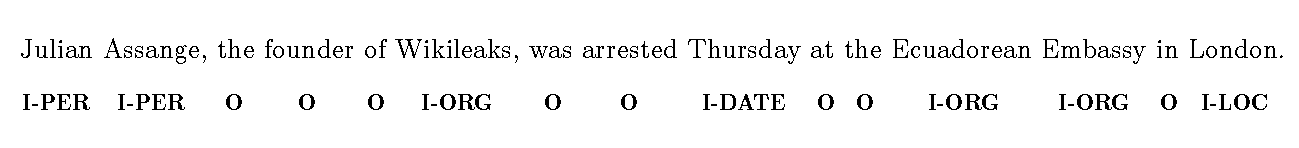
\includegraphics[width=1.0\textwidth]{pics/ner_example}
\caption{Named Entity Recognition as a sequence labeling task. The "O" stands for a token Outside a named entity.}
\label{fig:ner_example}
\end{figure}
%
Regular entities such as dates and prices can be extracted with almost perfect accuracy
using regular expressions, which are search patterns that describe a regular language and 
that can be easily implemented in most programming languages. Entities that belong to a 
limited set, such as the names of states in a country, can also be easily extracted with
simple dictionary matching. However, other types of entities, such as the ones investigated in
the {CoNLL-2003} challenge, require more sophisticated methods for sequence labeling.

Some traditional statistical methods that can label
complex entities with good accuracy are Hidden Markov Models~\citep{Bikel1999}, 
Maximum Entropy Markov Models~\citep{McCallum2000},
and Conditional Random Fields~\citep{Lafferty2001}. These statistical 
approaches have been frequently employed to sequence labeling tasks and still provide 
fairly good solutions because of their simplicity, speed and accuracy. However, they
are rapidly being replaced by Deep Neural Networks.

Recent research in deep learning has brought great advancements to NER. Some examples are
the LSTM-CRF~\citep{Huang2015} and neural character representations~\citep{Lample2016,Ma2016}. 
Deep learning differs from classical machine learning in
regard to the levels of abstraction learned by the classifiers. Deep learning techniques combine 
feature extraction and classification in a single system. While a conventional feed-forward
neural network may perform classification by learning the weights of a single hidden layer through
backpropagation, a deep learning model is usually composed of multiple hidden layers that handle 
different levels of abstractions. In text related tasks, the first level of abstraction usually
consists of a word embedding layer, where words are mapped to a continuous vectorial space with
reduced dimensionality, and the next layer usually consists of a multi-layered 
recurrent neural network or a convolutional neural network. 

Essentially all the best scoring models to date at the {CoNLL-2003} task employ some form of 
deep learning, and most often \gls{lstm}s. When combined with pre-trained
word embeddings, neural networks provide a powerful method of sequence labeling without
any feature engineering or dictionary matching. However, these models have 
become quite complex, contrasting with earlier approaches that
only required the estimation of a comparatively small number of weights. The training time
required by these deep models is many orders of magnitude longer than that of traditional approaches, 
and if we take into consideration the training of word embeddings such as Word2Vec's skip gram model 
in a billion token corpus~\citep{Mikolov2013}, the difference gets even more substantial. Additionally, 
deep learning models usually require expensive hardware for training to become practical options. 

In summary, the aforementioned sequence labeling models are exactly what we are looking for in the 
\gls{rne} task. By labeling tokens in a webpage with machine learning
models, we can extract researcher names with more flexibility than that provided by traditional 
tools for \gls{wde}.

\section{Researcher Name Extraction}
\label{sec:researcher_name_extraction}

The objective of this dissertation is to find the best sequence models for 
\gls{ner} on the Web by assessing their performance in the \gls{rne} task.
This task consists of extracting researchers names from university 
faculty listings across the world with the purpose of discovering their affiliations and linking 
their profiles to public databases such as DBLP or Google Scholar~\footnote{
  This is useful, for instance, if one needs to compare the research output of 
  departments in a country, or study international publication patterns.
}. Public researcher databases only have sparse information about author affiliation and,
even in fields for which the information is more easily available, such as Computer Science,
only a small fraction of the records have reliable affiliation information, as we have verified
in our preliminary studies. 
%
\begin{figure}
  \centering
  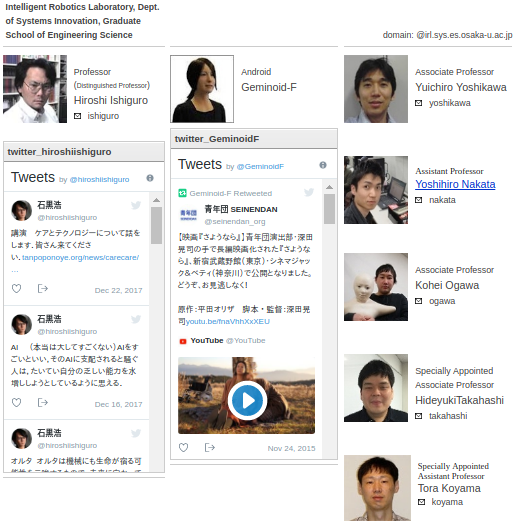
\includegraphics[width=0.65\textwidth]{pics/jap_osaka_lab}
  \caption{Example of a faculty webpage.}
  \label{fig:faculty_directory}
\end{figure}
%
To acknowledge the complexity of this task, take for example a snippet extracted from
the staff page for the intelligent robotics laboratory from Osaka University shown in 
Figure~\ref{fig:faculty_directory}.
There is some pattern to the way member profiles are arranged, but the organization is 
rather flexible. There are different character encodings in the page, there is some variation 
to the presentation style of each researcher data record
(some are links, some are text, the font varies, etc.), and also, even the laboratory's
android makes an appearance in a way that could be easily confused with a researcher.
Other pages, even from the same website, can show very different 
patterns, ranging from tables and lists to free form.
Researcher names can appear inside plain text, similar to the case of NER in
news texts or in a more tabular structure. Names may also be part of larger sentences such as in 
"Michael Johnson Chair" and "John Doe Avenue" yielding false positives. Or they can be composed 
of common words, e.g. Summer Hall, yielding false negatives. There is no extraction rule that can
fit all cases, so we need flexible solutions.

State-of-the-art \gls{ner} models trained on news datasets do not
perform well at this task, because in many webpages, textual information alone is insufficient to
indicate the semantic category of a word. The absence of context demands
extraction systems to rely on information from sources outside the text, being them 
features extracted from unlabeled corpora obtained through unsupervised pre-training, 
dictionaries containing instances of the relevant entities, HTML structural features, 
or other clever solutions. That is, 
a key problem in the task of entity name extraction is accounting for every
possible name combination. Since there is no database with all 
possible named entity combinations, we need holistic statistical methods that can handle 
unknown tokens with relative efficacy.
In Chapter~\ref{cha:dataset}, we introduce the \gls{rne} dataset to evaluate the 
performance of different sequence models in the \gls{rne} task.

Lastly, another important related task in the context of \gls{rne} is performing named 
entity disambiguation, which consists of linking the extracted named entities to a unique profile in a 
database. This task is called Named Entity Linking. In preliminary studies, we verified 
that roughly half the records found in faculty webpages can be linked to the respective records in public databases 
with the aid of string matching techniques. For the other half, we may need to employ more complex systems 
or perform manual classification. This task is also important, but it will not be covered in the present study.

\section{Summary}

This chapter discussed the broad problem of \gls{ie} in 
Section~\ref{sec:information_extraction}, presenting its challenges and relations to 
different fields of Computer Science, and showing how it encompasses the problem of 
\gls{wde}. Despite being a specific setting of \gls{ie}, \gls{wde} has specificities
that demand solutions that are different from those used for plain text.
In Section~\ref{sec:named_entity_recognition}, we discussed the related task 
of \gls{ner}, which is very useful to \gls{ie} both in plain text and 
Web extraction tasks. Recent developments in \gls{ner} can help \gls{wde} systems become
more flexible, handling extraction tasks across many website formats.
Lastly, in Section~\ref{sec:researcher_name_extraction}, we discussed the
problem of \gls{rne}, which is the main topic of this dissertation, 
showing how it can be challenging and why traditional solutions to \gls{wde} and \gls{ner}
may have difficulty handling this specific setting. In fact, by combining the valuable 
knowledge from both fields of study, we can get a more robust approach to \gls{rne}.


\chapter{Related Work}
\label{cha:related_work}

The \gls{rne} task is a problem in \gls{wde} that
we proposed to solve with the application of machine learning methods of \gls{ner}.
This chapter presents the related research in the fields of \gls{wde} 
in Section~\ref{sec:wde} and \gls{ner} in Section~\ref{sec:ner}.

\section{Web Data Extraction}
\label{sec:wde}

Since the early 1990s, the astonishing growth of public information in the Web has 
led to the development of a number of different approaches to the problem of \gls{wde}.
Traditionally, the task was solved by designing special purpose
programs called wrappers to recognize relevant data and store records in a structured
format. These early tools varied wildly relative to their degree of automation. 

It was readily perceived that manual wrapper generation was a rather tedious and
error prone process, unsuited for large scale operations. Wrappers tend to
break frequently because they rely on webpage features that can change 
often. So, in the late nineties, several authors advocated for wrapper induction, a technique 
that consists of automatically constructing wrappers from a small set of examples by 
identifying delimiters or context tokens that single out the desired attributes. 
Some remarkable wrapper induction methods are WIEN~\citep{Kushmerick2000}, Soft 
Mealy~\citep{Hsu1998} and STALKER~\citep{Muslea1999}.

Despite being better than constructing wrappers manually, wrapper induction methods 
still suffered from a lack of expressive power and flexibility. These methods had 
trouble handling records with missing attributes or unusual structures because
patterns could only be identified if they happened at least once in the examples.

Other approaches such as NoDoSE~\citep{Adelberg1998} and Debye~\citep{Laender2002a} 
brought greater flexibility to wrapper induction methods by requiring a greater level 
of human interaction through graphical user interfaces. \gls{wde} techniques often 
require some sort of assistance from human experts to boost accuracy. One of the main challenges 
in the field lies in determining an adequate trade-off between the degree of automation and 
the precision and recall of the data extraction tool.

To automate the task of \gls{wde} completely some approaches,
such as Road Runner~\citep{Crescenzi2001}, removed entirely the need for data examples.
Road Runner parses documents belonging to a same class (e.g. books in Amazon) and 
generates wrappers based on their similarities and differences, yielding comparable results 
to those obtained by wrapper induction methods. However, like previous approaches, it was 
unsuited for cross site extraction tasks because the learned rules were not general enough.

Early NLP-based approaches aimed at extracting more general rules that could possibly
be employed over multiple websites. RAPIER~\citep{Califf1999} is a method of rule
extraction that uses information such as part-of-speech tags and semantic classes from
a lexicon to derive patterns from a set of training examples. This approach is more
flexible than the wrapper induction methods, however it achieves much lower rates of 
precision and recall.

In 2002, a survey~\citep{Laender2002} made a thorough classification of the
early approaches with a taxonomy based on their main technology, being them: languages for
wrapper development, HTML-aware tools, NLP-based tools, Wrapper Induction Tools,
Modeling-based tools and Ontology-based tools. Some noteworthy examples from this era
are: 
%
\begin{itemize}
\item TSIMMIS~\citep{Hammer1997} and WebOQL~\citep{Arocena1999}, which are special purpose 
languages for building wrappers.
\item Road Runner~\citep{Crescenzi2001}, XWRAP~\citep{Liu2000} and W4F~\citep{Sahuguet1999}, 
which are HTML-aware tools that infer meaningful patterns from the HTML structure.
\item RAPIER~\citep{Califf1999}, SRV~\citep{Freitag1998}, WHISK~\citep{Soderland1999}, which 
are NLP-based tools.
\item WIEN~\citep{Kushmerick2000}, Soft Mealy~\citep{Hsu1998} and STALKER~\citep{Muslea1999} which 
are wrapper induction methods.
\item NoDoSE~\citep{Adelberg1998} and Debye~\citep{Laender2002a}, which are semi-supervised
tools that require some interaction with the user by means of a graphical
user interface.
\end{itemize}
%
% Text Runner.
% https://www.aaai.org/Papers/IJCAI/2007/IJCAI07-429.pdf
\cite{Chang2006} complemented the previous surveys with semi-supervised 
technologies such as Thresher~\citep{Hogue2005}, IEPAD~\citep{Chang2001} and 
OLERA~\citep{Chang2004}. They differed from supervised 
and unsupervised methods because they either needed only a rough description of
data from users for extraction rule generation or some level of post processing
that needed user attention. 
%The survey also mentioned newer unsupervised methods
% such as DeLa~\citep{Wang2003}, Exalg~\citep{Arasu2003} and Depta~\citep{Zhai2005}.

Most of the early \gls{wde} systems were rule-based with either 
manual rule description or automatic rule learning from examples, thus they
suffered from a lack of flexibility when dealing with noisy and unstructured data.
Huge progress in the field of statistical learning led to the development of
models that tried to solve this problem.

\cite{Sarawagi2008} introduced a classification that segmented wrappers in
rule-based methods, statistical methods and hybrid models, bringing together 
the fields of \gls{ner}, Relationship Extraction and \gls{wde}. 
The rule based methods encompass most of the previous models. While the statistical methods 
convert the extraction task into a token labeling task, solved with \gls{ner} 
and Relationship Extractions methods. Traditionally, these subtasks were solved with 
generative models based on \gls{hmm}s or discriminative models based on the 
Maximum Entropy principle, but recently these have been largely superseded by Deep Neural 
Networks. Different from automatic wrapper generators, statistical methods are suitable for
a large variety of tasks, especially when we want the system to handle cross website information 
extraction and plain text information extraction. That is why this class of methods is of 
special interest to our application. The progress of statistical models will be 
discussed in Section~\ref{sec:ner}.

Surveys by~\cite{Ferrara2014}, \cite{Schulz2016} and \cite{Varlamov2016} updated the 
previous surveys on Information Extraction methods with some interesting innovations. 
Some examples are: the Visual Box Model~\citep{Krupl2005}, a data extraction system that produces 
a visualization of the webpage to exploit visual cues to identify records presented in a tabular form;
automatic wrapper adaptation~\citep{Ferrara2011}, a technique that tries to reduce the cost of 
wrapper maintenance by measuring the similarity of HTML trees and adapting
wrappers to the new page structure; AutoRM~\citep{Shi2015}, a method to mine
records from a single webpage by identifying similar data regions through DOM
tree analysis; and Knowledge Vault~\citep{Dong2014}, a method that combines different 
extraction approaches to feed a probabilistic knowledge base.

Most data extraction systems focus on extracting information from single websites
and are therefore unsuited for cross website extraction tasks. Even unsupervised
approaches that are application domain independent, such as RoadRunner and EXALG, 
only work well when extracting data from pages generated from a same template. 

A statistical approach to unsupervised domain 
independent \gls{wde} was described by~\cite{Zhu2005}. The 2D CRF 
model takes a webpage segmented into data blocks and employs a two dimensional \gls{crf}
model to perform attribute labeling. The model was further improved 
in~\cite{Zhu2006} to model record segmentation and attribute labeling as a joint task.
Some of the limitations of early unsupervised methods 
were also addressed by ObjectRunner~\citep{Abdessalem2010} and AMBER~\citep{Furche2012}. 
These methods work by annotating webpages automatically with regular expressions, gazetteers and 
knowledge bases. They can rectify low quality annotations and even improve the annotators
by exploring regular structures in the DOM during the record segmentation phase.

\gls{wde} methods have undoubtedly improved extraordinarily, but
as pointed by \cite{Schulz2016}, it is difficult to compare the results 
achieved by competing tools. Also, many tools seem to rely excessively on heuristic methods.
The recent advancements in sequence taggers may provide more robust and flexible techniques
to address this problem.


\section{Named Entity Recognition}
\label{sec:ner}

\gls{ner} is an important subtask in \gls{ie}.
The \gls{ner} task was defined in the Third Message 
Understanding Conference (MUC-3)~\citep{Sundheim1991}, where researchers were asked to extract
entities from a news corpus about terrorist incidents. However, it was the 
language-independent \gls{ner} shared task at the Conference 
on Computational Natural Language Learning in 2003 ({CoNLL-2003})~\citep{KimSang2003},
that established an enduring labeled dataset constructed with news texts from Reuters.
Despite its reduced size and the limited variability of its documents, the {CoNLL-2003}
dataset is still used to compare the performance of NER systems in English and 
German. 

Sequence labeling for \gls{ner} and \gls{pos} tagging (labeling nouns, verbs, pronouns, etc.) 
is very similar, so, many times, research articles that propose new methods for \gls{ner}
also report results for the \gls{pos} Tagging task. And frequently, the best methods for 
\gls{pos} Tagging are also the best methods for \gls{ner}.

Traditionally, the \gls{ner} task was solved with generative models based on 
\gls{hmm}s. The first appearance of \gls{hmm}s in the
field of \gls{nlp} occurred in the mid-seventies and was
primarily focused on the problem of Speech Recognition. 
But in the late nineties, \gls{hmm}s also found important applications in \gls{ie}
and \gls{ner} as in the works by~\cite{Bikel1999}, 
\cite{Freitag1999}, and \cite{Freitag2000}.

The problem with \gls{hmm}s is that they model the joint probability between 
sequences of observations and labels $ P(X, Y) $, a harder problem than modelling the corresponding 
conditional probability $ P(Y|X) $. They assume conditional independence for the observations $ X $, and
therefore, they cannot handle overlapping features. This lack of flexibility led to the 
development of discriminative approaches to sequence labeling based on the Maximum Entropy principle.

Some early examples are Maximum Entropy Taggers for NER~\citep{Borthwick1998} and
\gls{pos} Tagging~\citep{Ratnaparkhi1998}. The Maximum Entropy Markov Model~\citep{McCallum2000} 
was developed just a while later, building up on the intuition of \gls{hmm}s combined with
the flexibility of discriminative approaches. However, because of the label bias problem,
this model was superseded by \gls{crf}s~\citep{Lafferty2001, McCallum2003}. 
At this time, the best performing systems almost always resorted to external gazetteers 
and hand-chosen features, as is the case for the {CoNLL-2003} winning model~\citep{Florian2003}.

With the advancement of Machine Learning in recent years, we saw the rise
of Neural Networks applied to sequence labeling. In 2011, \cite{Collobert2011} 
introduced Neural Networks free of feature engineering to sequence labeling tasks,
using \gls{cnn} over word embeddings with a CRF output layer to tackle 
the problems of \gls{pos} tagging, Chunking, Semantic Role Labeling, and NER. A similar architecture 
proposed in 2015 by~\cite{Huang2015}, the Bi-LSTM-CRF, replaced the \gls{cnn} in \cite{Collobert2011} 
with a bidirectional LSTM, achieving better results.

In 2016, further advancement to the NER models was achieved by incorporating character 
representations at the bottom of the Bi-LSTM-CRF architecture to extract morphological 
features from words automatically. The model by~\cite{Lample2016} uses a 
bidirectional \gls{lstm} over character embeddings and the model by~\cite{Ma2016} uses a
one dimensional \gls{cnn} with max pooling over character embeddings. Both models also 
made use of pre-trained GloVe word embeddings, created by~\cite{Pennington2014}.

Small improvements to NER systems have been made since then, primarily due to the 
introduction of new word embeddings on variations of the Bi-LSTM-CRF architecture. From
this group, we can mention ELMo~\citep{Peters2018}, BERT~\citep{Devlin2018}, and
Flair~\citep{Akbik2018}. 
All of them were introduced in 2018 and they differ primarily 
in how to construct contextual embeddings from the internal states of a language 
modelling neural network.

To our knowledge, the best NER system up to this date (considering the performance in the
{CoNLL-2003} dataset) is the bidirectional transformer model proposed by~\cite{Baevski2019} that uses
a stack of self-attention modules and ELMo embeddings. Table~\ref{tab:ner_model_comparison}
shows a comparison of the history of reported F1 scores in the English test set of the {CoNLL-2003} dataset
for the NER systems that were mentioned in this section. Each of the mentioned systems held the 
record for the task at a given time.

\begin{table}[h]
  \small
  \begin{center}
    \begin{tabular}{ lc }
      \toprule
      Model & Test F1 \\
      \midrule
       \cite{Florian2003} ({CoNLL-2003} Winner)    & 88.76 \\
       \cite{Collobert2011}                        & 89.59 \\
       \cite{Huang2015}                            & 90.10 \\
       \cite{Lample2016}                           & 90.94 \\
       \cite{Ma2016}                               & 91.21 \\
       \cite{Peters2018}                           & 92.22 \\
       \cite{Devlin2018}                           & 92.80 \\
       \cite{Akbik2018}                            & 93.09 \\
       \cite{Baevski2019}                          & 93.50 \\
      \bottomrule
    \end{tabular}
  \end{center}
  \caption{Model performances in the {CoNLL-2003} English test set.}
  \label{tab:ner_model_comparison}
\end{table}


\section{Summary}

In this chapter, we discussed the related work in \gls{wde} and \gls{ner}. 
The models discussed in this dissertation and employed in
the experiments section are methods for \gls{ner} that were each deemed the best machine learning 
techniques for solving the problem at a given time. However, the \gls{rne}
task is essentially a \gls{wde} task, so some ideas from this field are extremely useful, 
such as using HTML structural features, as we did in the Self-Training strategy for 
HMMs and the attention models for Neural Networks, that will be introduced in later chapters. Also, 
\gls{ner} is a subtask that is mostly useful when we think of it in the context of a larger task,
such as a specific setting of \gls{wde}. Because, \gls{ner} approaches may be more or less effective
depending on the objective extraction task. For example, we will see in the experiments section 
that, despite the significant improvements brought by ELMo embeddings to NER in plain text
(as attested by the results reported in the {CoNLL-2003} English dataset), their performance is far
from great when we consider the \gls{rne} task, being surpassed by much simpler
methods.


\chapter{Techniques for Sequence Labeling}

Many tasks in \gls{nlp}, such as \gls{pos} Tagging and \gls{ner}, can be 
solved by attributing labels to sequences of words. While in \gls{ner}, we 
want to classify words into a set of predefined labels, any sequence labeling 
task in \gls{nlp} can be modeled generically by considering that $ X = \{X_1, X_2, \ldots, X_n\} $ 
is a sequence of random variables representing words from a finite vocabulary
$ V = \{ a, aardvark, \ldots, zebra \} $, and $ Y = \{Y_1, Y_2, \ldots, Y_n\} $ is a sequence of 
random variables representing labels attributed to these words that take values from
a finite set $ L = \{ \text{B-PER}, \text{I-PER}, ..., \text{O} \} $, with both sequences generated by an unknown 
probability distribution. Considering that we observe the sequence of words $ x $ but 
we do not observe the sequence of labels $ y $, then the goal for our classifier is to find: 
%
\begin{equation}
\label{eq:1}
y^* = \argmax_{y} P(Y=y|X=x)
\end{equation}
%
That is, the sequence of labels $ y^* $ that maximizes the conditional probability of
$ y $ once we have observed the sequence of words $ x $. 

% For example, in a \gls{ner} 
% setting, after observing the sentence \{ John, Smith, is, a, man \} we could conclude 
% with a good probability model that the corresponding label sequence \{ I-PER, I-PER, O, O, O \} 
% has the highest probability.

Estimating $ P(Y|X) $ naively from the relative frequencies in a labeled corpus 
is usually inadequate due to the exponential increase in the number of word and label combinations that 
needs to be considered as we increase the sequence size $ n $. As $ n $ becomes large, label combinations 
will become increasingly uncommon in the dataset, what makes probability estimation less reliable. For
example, if the vocabulary size consists of 1,000 words and there are three possible labels for each 
word, then there are already 27 billion combinations for sequences of only three words and labels.
Also, sequences that were not seen during training will always have zero probability. That is problematic, 
because proper names are often unique or very infrequent in a corpus,
so many word sequences that we care about will belong to this category.

Ultimately, the difference between statistical sequence labelling models lies in the assumptions 
that we make about the distribution $ P(Y|X) $. For practical reason, most statistical models of natural language make 
simplistic assumptions about the language structure. For example, a common assumption that is 
shared to some extent by all the models presented in this chapter is the Markov Assumption, that will be 
discussed thoroughly in Section~\ref{sec:hmm}. Stated simply, it assumes that by looking at a limited 
history in the sequence, for example the two previous words, we have sufficient information to make accurate 
predictions about the current word's label. 

The related task in \gls{nlp} called Language Modelling consists of predicting the next 
word in a sequence by looking at the tokens that precede it. Using the Markov Assumption, 
a language model that looks at the two previous words is called a bigram model and a model that 
looks at the three previous words is called a trigram model.
%
\begin{quote}
For anyone from a linguistics background, the idea that we would choose to use a model of language structure
which predicts the next word simply by examining the previous two words - with no reference to the 
structure of the sentence - seems almost preposterous. But, actually, the lexical co-occurrence, semantic, and
basic syntactic relationships that appear in this very local context are a good predictor of the next word, and
such systems work surprisingly well. Indeed, it is difficult to beat a trigram model on the purely linear task
of predicting the next word~\citep{Manning1999}.
\end{quote}
%
Considering this, we do not usually evaluate the quality of statistical natural language models by how reasonable
their assumptions are, but by how instrumentally effective the models are for solving objective tasks. The 
epistemological implications of this view are important, but in this work we will consider it to be valid.

In this chapter, we discuss several machine learning methods for \gls{ner}. In Section~\ref{sec:hmm}, we discuss Hidden Markov 
Models, in Section~\ref{sec:crf} we discuss Conditional Random Fields, and in Section~\ref{sec:neural_networks} we 
discuss Neural Networks.


\section{Hidden Markov Models}
\label{sec:hmm}

In this section, we derive a supervised \gls{hmm} approach for \gls{ner}.
The \gls{hmm} is an expanded Markov Chain where the sequence of observed states
depends on an underlying sequence of hidden states. In the context of \gls{ner}, we can 
think that the states of a Markov Chain correspond to the set of possible labels 
or classes (e.g. PER, ORG, LOC, etc.). First, we consider a standalone Markov Chain and then
we proceed to discuss \gls{hmm}s.

A Markov Chain is a stochastic 
model for describing sequences when the described sequences have the Markov Property. That is, 
consider a sequence of random variables $ Y = \{Y_1, Y_2, \ldots, Y_n\} $ 
taking values from a restricted set of possible states
$ L = \{L_1, L_2, \ldots, L_m \} $. Sequence $ Y $ only satisfies the Markov Property if:
%
\begin{equation}
P(Y_i=L_k|Y_{i-1}) = P(Y_i=L_k|Y_{i-1}, Y_{i-2}, \ldots, Y_1)
\end{equation}
%
The probability of observing state $ Y_i=L_k $ depends only on the previous state.
What the Markov Assumption implies is that, at any position in the sequence, the entire history 
of observed states is encoded in the previous state. So, by knowing the
previous state, we can make as accurate predictions about the future as we would make by 
knowing all the history. Conditioned on this previous state, the future and past states 
are independent. 

When we consider two or three previous states instead of a single previous state,
the Markov Chain is said to be of second order and third order, respectively.
Any Markov Chain of higher order can be converted into an equivalent first order Markov 
Chain. For example, a Markov Chain of second order with two states $ \{A,B\}$ can be transformed 
into an equivalent Markov Chain of first order with four states $ \{ AA, AB, BA, BB \} $. Therefore, 
from now on, we will proceed with the analysis of first order Markov Chains without loss of generality
regarding higher order Markov Chains.

A Markov Chain can represent a wide range of phenomena such as daily temperatures in a region, 
closing prices of a stock in the financial market, yearly demographic growth, or words in a text. 
However, in all these cases, the model is a simplification of reality that makes sequences mathematically 
treatable. The extent to which this simplification will hurt our predictions depends on the 
nature of the studied phenomena. 

To see why assuming the Markov property may introduce a problem on text related tasks, consider the following
labeled sentence: 
%
\begin{quote}
"[Jon Snow]$_{PER}$ is [Ned]$_{PER}$ 's son. Snow is piling up over [Winterfell]$_{LOC}$, but [Snow]$_{PER}$ is not bothered."
\end{quote}
%
Snow is a very uncommon name, so a statistical model may have difficulty labeling the last mention of Snow correctly,
but it would certainly be helpful if it could refer to the first mention in the beginning of the sentence,
where the named entity label is more obvious. To do this we would need to keep track of distant relationships in 
the text that would not be captured by a Markov Model of second or third order. While we could consider
employing a Markov Model of higher order to overcome this limitation, 
considering more than three or four states at any time makes parameter estimation unreliable
because each combination of states becomes increasingly uncommon in the training set. Also, 
when the considered number of states increases, the cost for predicting the optimal sequence 
of states quickly becomes prohibitively high. 
There are some Markov Chain variations that try to address this problem, 
as well as the other models presented later in this chapter.
However, HMMs up to third-order can work well if 
we add independent features to make up for the lack of a longer context. 

Furthermore, besides the Markov Assumption, we make the Time Invariance Assumption:
%
\begin{equation}
P(Y_{i+1} = L_b |Y_{i} = L_a) = P(Y_i = L_b |Y_{i-1} = L_a)
\end{equation}
%
That is, given the observed states $ L_a $ and $ L_b $, the probability of 
going from $ L_a $ to $ L_b $ in position $ i $ is the same as in any other position in 
the sequence. 
We refer to "time" invariance eventhough the correct name for this assumption
in the context of sequence labeling would be positional invariance, because
this is the usual name adopted in the literature. Everytime we refer to time or 
timesteps in the text, we mean the position of a token or label in the sequence.

% For the sake simplicity, assume that, unless clearly stated, the random
% variables $ Y_i $ refer to $ Y_i=L_k $ 
With this, we can calculate the probability of observing sequence
$ {{ Y = \{ Y_1, Y_2, ..., Y_n \} }} $ as:
%
\begin{equation}
P(Y) = \prod_{i=1}^{n} P(Y_i|Y_{i-1}) \\
\end{equation}
%
With the Time Invariance Assumption, all transition probabilities in our model can be described 
by a $ |L| \times |L| $ transition matrix $ \theta $ where each element $ \theta_{a, b} $ with
row $ a $ and column $ b $ holds the probability of going from state $ L_a $ to $ L_b $ and
$ |L| $ is the number of possible labels.
Naturally, the probabilities of row $ \theta_{a, *} $ must sum up to one since they represent
the entire scope of transition possibilities starting from state $ L_a $. For example,
consider the finite state-machine in Figure~\ref{fig:markov_graph} that describes 
a Time Invariant Markov Chain with only two states (Name, Word), that models a sequence 
of words that can be either names or common words. The edges in this graph represent the transition
probabilities between states and the transition matrix for this Markov Chain takes the form:
%
\begin{equation*}
\theta = 
\begin{bmatrix}
    0.3 & 0.7 \\
    0.4 & 0.6 \\
\end{bmatrix}
\end{equation*}
%
\begin{figure}
\centering
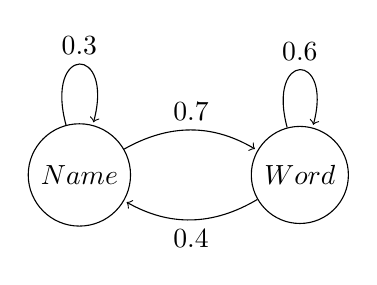
\begin{tikzpicture}[->,shorten >=1pt,auto,node distance=2.8cm]
  \tikzstyle{every state}=[]

  \node[state] (A)              {$ Name $};
  \node[state] (B) [right of=A] {$ Word $};

  \path (A) edge [loop above] node {0.3} (A)
            edge [bend left]  node {0.7} (B)
        (B) edge [bend left]  node {0.4} (A)
            edge [loop above] node {0.6} (B);
\end{tikzpicture}
\caption{Finite state machine for a Markov Chain.}
\label{fig:markov_graph}
\end{figure}
%
If we know the transition matrix $ \theta$ for a Markov Chain, we can easily calculate 
the probabilities of being in each state at time $ t $. If $ \rho_t $ is a vector of 
size $ m $ with the probabilities for each state at time $ t $. Then:
%
\begin{equation}
\rho_{t} = \rho_0 \cdot \theta^t
\end{equation}
%
Where $ \rho_0 $ is the vector of starting probabilities for each state. We assume that we 
have no knowledge about the initial probabilities of our Markov Chain, so we simply 
attribute the same probability to every state at time $ t=0 $. For the Markov Chain described
in Figure~\ref{fig:markov_graph}, this assumption would make $ \rho_0 = ( 0.5, 0.5 ) $. 
For convenience, consider that $ P(Y_1|Y_0) $ 
is the probability of $ Y_1 $ given the initial vector of uniform state
probabilities $ \rho_0 $. 

Now we know how to calculate the state probabilities for a Markov Chain at any position in the sequence
provided that we know the transition matrix. In the context of sequence labeling, we want
to obtain the transition matrix $ \theta $ from our training data.
The most usual choice is to obtain $ \theta $ such that it maximizes the probability of reproducing 
our labeled dataset with Maximum Likelihood Estimation. More formalliy, the likelihood of our model 
is given by:
%
\begin{equation}
\mathcal{L}(\theta) = \prod_{i=1}^{n} \theta_{y_i, y_{i-1}}
\end{equation}
%
Where $ y_i $ is the correct label at position $ i $.
By defining $ \eta_{a,b} $ to be the count of transitions from state 
$ a $ to $ b $ in the dataset, where $ a $ and $ b $ are states
from a finite set of states $ L = \{ L_1, L_2, \ldots, L_k \} $. Instead, we can write the likelihood as:
%
\begin{equation}
\mathcal{L}(\theta) = \prod_{a, b \; \in \; L} \theta_{a, b}^{\eta_{a, b}}
\label{eq:hmm_likelihood}
\end{equation}
%
where the product is calculated over all possible transitions from $ a $ to $ b $.
The logarithm function is monotone increasing, so we can maximize the log-likelihood instead
of the likelihood for ease of calculation. With the log-likelihood, the product over transition 
probabilities becomes a sum of logarithms. The log-likelihood is defined by:
%
\begin{equation}
\mathcal{l}(\theta) = \sum_{a, b \; \in \; L} \eta_{a, b} \cdot log(\theta_{a, b})
\end{equation}
%
Then, the maximum likelihood estimator becomes:
%
\begin{align}
\hat\theta = \argmax_{\theta} \mathcal{l}(\theta)
\end{align}
%
However, if we try to optimize this function as it is, we will find that
$ \hat\theta_{a, b} = \infty $. This happens because we did not
take into account the degrees of freedom of our model. Every row in the transition matrix must sum up to one,
so the parameters for the last row are defined by the preceding rows. The degrees of freedom 
for the model are actually $ |L|(|L|-1) $ and not $ |L|^2 $ as we were inadvertently considering before. 
That is, we have a set of constraints:
%
\begin{equation}
\sum_{b \; \in \; L} \theta_{a, b} = 1, \;\; \forall \; a \in L
\end{equation}
%
With the aid of Lagrange Multipliers, we can incorporate this set of constraints into our optimization 
objective and optimize the Lagrangian:
%
\begin{equation}
\Lambda(\theta, \lambda) = \mathcal{l}(\theta) - \sum_{a \; \in \; L} \lambda_{a} \cdot \left( \sum_{b \; \in \; L} \theta_{a, b} - 1 \right)
\end{equation}
%
Setting $ \frac{\partial \Lambda(\theta, \lambda)}{\partial \lambda_a} = 0 $ simply yields the initial set 
of constraints, but by setting the partial derivatives $ \frac{\partial \Lambda(\theta, \lambda)}{\partial \theta_{a, b}} = 0 $,
we get:
%
\begin{eqnarray}
\frac{\partial \Lambda(\theta, \lambda)}{\partial \theta_{a, b}} & = & \frac{\eta_{a, b}}{\theta_{a, b}} - \lambda_a = 0 \\
\theta_{a, b} & = & \frac{\eta_{a, b}}{\lambda_a}
\end{eqnarray}
%
Finally, using the initial constraint equations, we find that:
%
\begin{align}
\sum_{b \; \in \; L} \frac{\eta_{a, b}}{\lambda_a}  =  1 \\
\lambda_a                             =  \sum_{b \; \in \; L} \eta_{a, b} \\
\hat{\theta}_{a, b}                   =  \frac{\eta_{a, b}}{\sum_{b' \; \in \; L} \eta_{a, b'}}
\label{eq:theta_estimate}
\end{align}
%
yielding a closed form expression for the maximum likelihood transition matrix. What is really convenient, 
since this is the average number of transitions from state $ a $ to state
$ b $ in the dataset. A value that can be easily calculated.

So far, we have assumed that all states/labels are observable, but in \gls{ner}, only the words 
are observed, while the named entity labels associated with these words are not. That is why we need
another layer of complexity. The \gls{hmm} differs from the Markov Chain in that it 
does not observe the states $ Y $ directly, but rather a probabilistic function of these states.
In Markov Chains, only the labels were being considered without 
mention of the accompanying words. With the \gls{hmm}, we want to estimate the probabilities of 
a sequence of labels $ Y = \{Y_1, Y_2, ..., Y_n\} $ 
(i.e. the Markov Chain) from a sequence of observed states $ X = \{X_1, X_2, ..., X_n\} $
(i.e. the words in a text, or a feature vectors with independent features). 
Now, to calculate the conditional probability for a sequence of labels we employ 
Bayes Theorem:
%
\begin{equation}
P(Y|X) = \frac{P(X|Y) P(Y)}{P(X)}
\end{equation}
%
Also, since $ P(X) $ is invariant for every sequence of labels $ Y $, to find the 
most likely sequence of labels, we can simply optimize in terms of the joint probability:
%
\begin{equation}
P(Y|X) \propto P(X|Y) P(Y) = P(X, Y)
\end{equation}
%
The procedure to obtain the $ P(Y) $ probabilities has already been described for the 
standalone Markov Chains and it is the same for \gls{hmm}s. But, to obtain the $ P(X|Y) $ 
probabilities, we must make another assumption. That is:
%
\begin{equation}
P(X_i=x_i|Y_i=y_i, Y_{i-1}=y_{i-1},X_{i-1}=x_{i-1}, ...) = P(X_i=x_i|Y_i=y_i)
\end{equation}
%
the probability of observing word $ x_i $ depends only on the current label
$ y_i $, the hidden state (e.g. B-PER, I-PER, O, etc.). With this assumption, we are
stating that once we know a token's assigned label, then we can reliably predict what is the 
probability that this token takes any value from a limited vocabulary. Conditioned on the assigned
label, the current word is independent of the other words in the sequence.
This assumption is problematic when we want to use observations from other positions in
the sequence to predict labels at the current position, because these observations are
likely to be correlated. For this reason, other models such as \gls{crf}s (explored in the next section) 
try to overcome this issue by taking different assumptions. 

Now we can finally calculate the probability of a sequence $ Y $ given a sequence of 
observations $ X $:
%
\begin{equation}
P(Y|X) \propto \prod_{i=1}^{n} P(X_i|Y_i)P(Y_i|Y_{i-1}) \\
\end{equation}
%
This is the main equation for the \gls{hmm}.
To model the emission probability distributions $ P(X_i|Y_i) $, we assume that 
the probabilities are time invariant and that $ X_i $ takes its value from a fixed vocabulary 
with size $ |V| $. Similar to the transition matrix $ \theta $, we introduce a $ |V| \times |L| $ 
emission matrix $ \mu $, where $ |L| $ is the number of possible labels and each cell $ \mu_{a,b} $ represents the probability that, 
given label $ a $, we will observe word $ b $. For example, consider the
finite state-machine in Figure~\ref{fig:hidden_markov_graph} that extends our previous 
example and defines a \gls{hmm} with two states (Name, Word), and a vocabulary of 
two words (John, Hall). The edges between the hidden states and the words represent the emission probabilities,
and the emission matrix for this HMM takes the form:
%
\begin{equation*}
\mu = 
\begin{bmatrix}
    0.9 & 0.1 \\
    0.2 & 0.8 \\
\end{bmatrix}
\end{equation*}
%
\begin{figure}
\centering
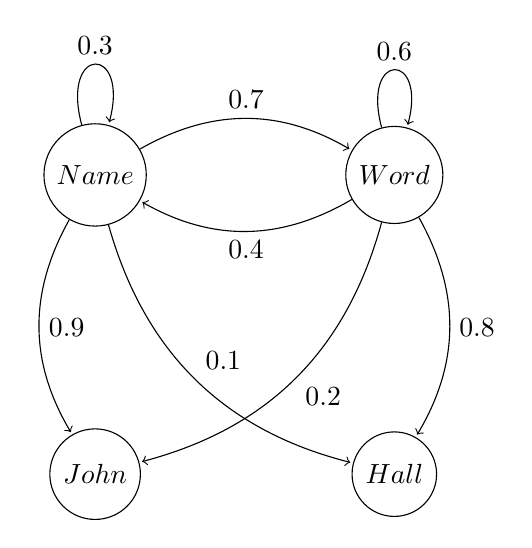
\begin{tikzpicture}[->,shorten >=1pt,auto,node distance=3.8cm]
  \tikzstyle{every state}=[]

  \node[state] (A)              {$ Name $};
  \node[state] (B) [right of=A] {$ Word $};
  \node[state] (C) [below of=A] {$ John $};
  \node[state] (D) [below of=B] {$ Hall $};

  \path (A) edge [loop above] node {0.3} (A)
            edge [bend left]  node {0.7} (B)
            edge [bend right] node {0.9} (C)
            edge [bend right] node {0.1} (D)
        (B) edge [bend left]  node {0.4} (A)
            edge [loop above] node {0.6} (B)
            edge [bend left] node {0.2} (C)
            edge [bend left] node {0.8} (D);
\end{tikzpicture}
\caption{Finite state machine for a Hidden Markov Model.}
\label{fig:hidden_markov_graph}
\end{figure}
%
Now the log-likelihood for the \gls{hmm} is defined as:
%
\begin{equation}
\mathcal{l}(\theta, \mu) =
\sum_{a \; \in \; L, b \; \in \; L} {\eta_{a, b}} \cdot log(\theta_{a, b}) +
\sum_{c \; \in \; L, d \; \in \; V} \eta'_{c, d} \cdot log(\mu_{c, d})
\end{equation}
%
where $ \eta'_{c, d} $ is a function that counts the number of emissions from state $ c $
to word $ d $. The matrices $ \theta $ and $ \mu $ are independent, so we can optimize for
the transition and emission matrices separately, therefore the procedure to find $ \hat\theta $ 
is still the one described in Equation~\ref{eq:theta_estimate}. Also, notice that
if we do the same procedure with Lagrangian Multipliers that we employed to find the MLE 
for Markov Chains, but this time we take the partial derivatives relative to 
$ \mu_{c,d} $ and set the constraints such that each line in the emission matrix must sum up
to one, we will find that:
%
\begin{equation}
\hat{\mu}_{c, d} = \frac{\eta'_{c, d}}{\sum_{d' \; \in \; V}\eta'_{c, d'}}
\label{eq:mle_words}
\end{equation}
%
This is the expected number of times that we observed word $ d $ when we were at the hidden state $ c $
in the training set. 
A closed form expression that is easy to calculate from the training data. With that, we conclude 
the maximum likelihood parameter estimation for the \gls{hmm}. This procedure is
only usable when we have access to labeled data, since we need to observe the correct labels 
to estimate $ \hat\theta $ and $ \hat\mu $. If we only have unlabeled data or partially labeled data, 
we can do the parameter estimation with the Baum-Welch Algorithm by~\cite{Baum1970}, though the results for 
NER become much less reliable.


\subsection{Smoothing}

The problem with the Maximum Likelihood Estimator derived above is that the emission probability for 
words that were not observed in the training set will always be zero. Considering that we only have a 
small dataset and even if it were much bigger we would still observe new words when running predictions
for unseen data, this problem needs to be addressed. We use Laplace smoothing~\citep{Manning1999} to change 
the estimates for $ \theta $ and $ \mu $ attributing some probability mass to unseen tokens:
%
\begin{align}
\hat{\theta}_{a, b}    =  \frac{\eta_{a, b} + 1}{\sum_{b' \; \in \; L} \eta_{a, b'} + |L|} \\
\hat{\mu}_{c, d} = \frac{\eta'_{c, d} + 1}{\sum_{d' \; \in \; V}\eta'_{c, d'} + |V|}
\end{align}
%
where $ |L| $ is the number of labels and $ |V| $ is the size of the vocabulary. 
If we consider other smoothing methods we will get different estimators, 
but this already properly ensures that unobserved words will not receive a zero 
probability. The main shortcoming with Laplace Smoothing is that it gives too 
much probability mass to unseen words relative to other smoothing methods.


\subsection{Predicting sequences}

The last task that needs to be done is to calculate the most likely sequence of labels given a sequence of
observations. With estimates for transition and emission matrices we can easily calculate the conditional
probability $ P(Y=y|X=x) $ of each label sequence $ y $, given the observed sequence $ x $. But, instead of 
computing probabilities for each possible label configuration and taking the one with maximum probability,
we can obtain the label sequence with maximum probability with the Viterbi algorithm by~\cite{Forney1973}, which is a dynamic 
programming algorithm that calculates the probabilities for sequences with the Markov Property exactly and efficiently.
As we increase the order of our HMM, this computation becomes exponentially more expensive,
but we found experimentally that for HMMs up to third order, the Viterbi algorithm is still viable. For larger windows,
a beam-search strategy can be used. 

\subsection{Self-Training} 
\label{sec:self_training}

%%% @ Review 4
%%% Rewrite self-training explaining the intuition further.

A \gls{hmm} for the sequence labeling task has the form:
\begin{equation}
P(y|x) \propto \prod_{i=1}^n P(x_i|y_i) P(y_i|y_{i-1})
\end{equation}
where $ x $ is a sequence of words and $ y $ is a sequence of labels, both with size $ n $,
and the initial probabilities $ P(y_1|y_0) $ follow a uniform distribution across all label 
assignments. Also, to simplify the notation, we omit the random variables, that is,
$ {{ P(Y=y|X=x) \equiv P(y|x) }} $.
To construct this model from the data, we need to estimate the following probabilities:
%
\begin{itemize}
  \item $ P(x_i|y_i) $: the emission probability of word $ x_i $ given label $ y_i $.
  \item $ P(y_i|y_{i-1}) $: the transition probability of going from label $ y_{i-1} $ to label $ y_i $.
\end{itemize}
%
We may consider $ x_i $ to be a vector of binary features, i.e. $ x_i = \{ f_{i,1}, f_{i,2}, ..., f_{i,k} \} $
as long as all the feature distributions are independent, conditioned on $ y_i $. That is:
\begin{equation}
P(x_i|y_i) = P(f_{i,1}, f_{i,2}, ..., f_{i,k}|y_i) = \prod_{j=1}^k P(f_{i,j}|y_i)
\end{equation}
%
Also, due to the time invariance assumption, the $ P(f_{i,j}|y_i) $ probabilities 
are independent of the timestep $ i $. Therefore, for each binary feature $ f_j $ we
need only estimate the parameters $ \hat{P}(f_{j}|y) $, relative to each possible
assignment of $ y $.
The maximum likelihood estimators for these feature parameters can be obtained
from their relative frequencies, just as we did in Section~\ref{sec:hmm} for single words 
(Equation~\ref{eq:mle_words}). For example, consider a binary feature $ F_C $ that indicates
if a word is capitalized and label $ Y $ which takes a value from the set $ \{ PER, O \} $ 
indicating if the current word is a person name (PER) or something else (O), then we can get 
the feature estimator with the expression:
%
\begin{equation}
\hat{P}(F_{C}=1|Y=\text{PER}) = \frac{\text{Count}(f_{C}=1, y=\text{PER})}
{\text{Count}(f_{C}=0, y=\text{PER}) + \text{Count}(f_{C}=1, y=\text{PER})}
\label{eq:feature_mle}
\end{equation}
%
where $ \text{Count}(f_C=A, y=B) $ is a function that counts the number of times
feature $ f_C $ took value $ A $ at the same time that label $ y $ took
value $ B $ in the training set. 

This approach yields good experimental results for textual features such as the capitalization
of a word, but if we try to use HTML structural features such as the HTML tags, we will find that
they are not very useful, contradicting our intuition.
The problem is that there is not much similarity between the HTML structure in different webpages.
For example, only because a named entity label occurs more often inside <div> tags
in a page, this does not mean that will be the case for most webpages. Consider for example a faculty webpage 
that shows researcher names in a table (<td> tags) in contrast to a webpage that organizes researcher
names in a list (<li> tags). If there are many cases like the former page in our training set, and we use the 
HTML tag feature in a model that assigns labels to the latter page in our test set, we will probably get many 
wrong predictions.
Nonetheless, the HTML features are not useless. Inside a single webpage, the HTML tag is a good predictor
of the correct labels. Words with a similar HTML context tend to have similar labels. For example, words
that happen together in a list have very similar HTML contexts and are very likely to belong to
the same category. The question is how to obtain better parameter estimators for HTML features.

Consider a set $ T $ of $ m $ textual features unrelated to the HTML structure:
%
\begin{equation*}
T = \{ f^T_1, f^T_2, ..., f^T_m \}
\end{equation*}
%
And a set $ H $ of $ k $ HTML features that are related to the HTML structure:
%
\begin{equation*}
H = \{ f^H_1, f^H_2, ..., f^H_k \}
\end{equation*}
%
Given a \gls{hmm} trained with only the first set of features $ T $,
we can use this model to predict the labels for an unlabeled document. 
Consider an HTML binary feature $ F_{td} $ representing if a token's parent tag 
is <td>, then the estimator for this HTML feature probability becomes:
%
\begin{equation}
\hat{P}(F_{td}=1|Y=\text{PER}) = \frac{\text{Count}(f_{td}=1, \tilde{y}=\text{PER})}
{\text{Count}(f_{td}=0, \tilde{y}=\text{PER}) + \text{Count}(f_{td}=1, \tilde{y}=\text{PER})}
\end{equation}
%
Where $ \tilde{y} $ is the label predicted by the \gls{hmm} trained with only textual features and
$ f_{td} $ is the feature value in the training set.
We use this formulation to calculate feature probabilities for only the HTML features.
Next, we incorporate the estimators for the HTML feature probabilities in the original \gls{hmm} 
and predict the final labels with the whole set of features $ T \cup H $. 
This process could be repeated multiple times. If the predictions are becoming more accurate with
each iteration, then the estimates are also likely to improve. 

In a simpler explanation, the self-training strategy can be divided into the following steps:
%
\begin{itemize}
\item Train the HMM without any HTML features.
\item Compute labels for a website with the trained HMM.
\item Use the computed labels as a proxy for the actual labels in the 
website and estimate HTML feature frequencies for this website alone.
\item Recompute the labels now using the HTML feature probabilities.
\end{itemize}
%
To understand why this strategy could help labeling named entities on the Web, consider the 
example shown in Figure~\ref{fig:self_training}. This example shows a snippet from a webpage 
and how a naive \gls{hmm} would probably attribute 
labels to each word. Despite being rather uncommon, North West is an actual person name,
what becomes obvious in this case once we know the HTML context where it happens 
(inside a list with other person names), but this is not so obvious if we consider the
sentence in isolation. The naive \gls{hmm} could be improved if we calculated
feature probabilities for the parent tags using proxies for the correct labels. We would find
that four times in a total of six occurrences, the correct label for a word that happened inside
a \textit{<li>} tag was \mbox{\textit{I-PER}}. By incorporating this knowledge in the model 
using the self-training strategy, we would improve the probability that words North and West 
were labeled correctly as a person name in this case.

\begin{figure}
  \centering
  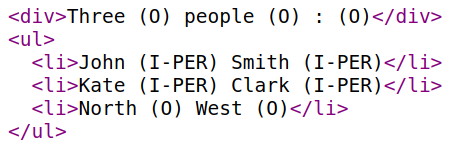
\includegraphics[width=0.5\textwidth]{pics/self_training_example}
  \caption{Example of a webpage snippet with labels attributed by a HMM.}
  \label{fig:self_training}
\end{figure}

This strategy could possibly be incorporated in the Baum-Welch algorithm to provide a more 
statistically solid argument for its effectiveness, but this heuristic
already yields a consistent improvement to sequence labeling on the Web. 
In theory, this 
strategy could be used with any sequence tagger, however retraining a classifier with new features can 
become prohibitively expensive in the case of CRFs or Neural Networks. 
In HMMs, retraining the features
is fast, because we assume feature independence and the maximum likelihood estimator can be 
obtained with a simple closed form expression.


\subsection{Experimental Considerations}

HMM based taggers have been successfully applied in many NLP and WDE tasks such as in the works by
\cite{Rabiner1990}, and \cite{Freitag2000}. The closed-form parameter estimation
makes them incredibly fast to train, also their parameters are very interpretable (because the model is simple), 
making them a good choice for a first approximation to NER. However, as we will discuss in the experiments section,
these models are highly dependent on the right selection of features, what may outweigh the 
benefit of a small training cost.


\section{Conditional Random Fields}
\label{sec:crf}

With \gls{hmm}s, we tried to model the joint probability between 
words and labels $ P(X, Y) $ and derive the conditional probability $ P(Y|X) $
with Bayes Theorem. However, this is a waste of modelling effort,
since we need to assume the shape of the prior distribution $ P(Y) $, but we 
only really care about the conditional problem. Thus, modelling $ P(Y|X) $ 
instead of the joint distribution would presumably be a more direct and simple 
approach. Also, to assure that the computation of $ P(X, Y) $ was feasible, we 
needed to assume feature independence, what inhibits the use of overlapping 
features that could potentially be useful in addition to words. Maximum Entropy
models for sequence labeling were created to address these issues and, among 
them, Linear Chain \gls{crf}s~\citep{Lafferty2001} stand out 
as the discriminative analogue to \gls{hmm}s. \gls{crf}s estimate the conditional probability 
while \gls{hmm}s, being generative models, estimate the joint probability. In this section,
we derive the Maximum Entropy Classifier and the Linear Chain \gls{crf} from basic 
principles.

The concept of Information Entropy established by~\cite{Shannon1948}
quantifies the amount of information expressed in a statistical distribution. 
The entropy $ H $ of a random variable Z with a probability mass function 
$ P $ is given by:
%
\begin{equation}
H(Z) = \sum_{z \; \in \; Z} P(z) \cdot log \left( \frac{1}{P(z)} \right)
\end{equation}
%
The logarithm in the entropy function can be taken in any base. The change 
of base will only provide a linear scaling of the same entropy function. When using base two,
$ H(Z) $ is essentially the expected number of bits necessary to encode the value of a
random outcome drawn from $ Z $, that is $ E \left[log \left( \frac{1}{P(Z)} \right) \right] $.
The more bits we need to use to encode the possible outcomes of a probability mass function, 
the more uncertain we are about the underlying distribution. For example, if an event has
only one possible outcome, we always know the value of a random sample, therefore
$ H(Z) = 0 $ and the entropy is minimum. On the other end, if the probability distribution is
uniform, all outcomes have the same probability, and therefore we are as uncertain as we can be
and the entropy is maximum.

The principle of maximum entropy set forward by~\cite{Jaynes1957} states that, when we do not know exactly what probability 
distribution generated a sample, the best estimate for the parameters of this probability
distribution is the one that makes the least assumptions, or the one with maximum entropy. 
This is the distribution that is closest to the uniform distribution. 
A similar argument can be made to limit the number of free parameters in the model. That is,
when comparing two models with similar predictive power, the one with the least degrees of 
freedom should be preferred. 

The principle of maximum entropy is similar to a principle in the philosophy of science called Occam's Razor~\footnote{
This idea is attributed to the English scholar William of Ockham that lived in the thirteenth century.
}, 
that states that, when there are two explanations for an outcome, the one that makes
the least number of assumptions is the best. Which is a good rule of thumb for science in general,
even though, ultimately, nothing guarantees that simpler models will be better.

The task of labeling word sequences can be thought of as a multinomial classification task where 
each label $ Y $ is predicted according to its context $ X $. The random variable $ Y $ takes
values from a finite set of labels $ L = \{ L_1, L_2, \ldots, L_k \} $ and the random variable
$ X $ takes a value from a finite set of possible contexts $ C $. These contexts are defined by 
a vector of observations expressing features (useful pieces of evidence) such as: the last word 
is an honorific, the current word is capitalized, the current word is "that", etc. Also, we
define $ k $ binary feature functions $ f_j \; \forall j \; \in \; [1, k] $ such that:
%
\begin{equation}
  f_j(x, y) = \begin{cases} 
    1 \text{ if } y = L_a \text{ and the feature is present in } x \\ 
    0 \text{ otherwise}
  \end{cases}
\end{equation}
%
Where the feature function is only true when the observed label is $ L_a $ and the feature
occurs in context $ x $.
So, at any position in the sequence, the truth statement of the feature functions can be
determined in terms of the predicted label $ y $ and the context $ x $. At this moment,
we treat the task of attributing labels to tokens at each position independently, so we 
consider that the context $ x_i $ and label $ y_i $ for a token at
position $ i $ can simply be represented generically by $ x $ and $ y $.

Now, the Maximum Entropy framework 
provides a compelling way for estimating the probability of a label given its linguistic context, 
that is $ P(Y|X) $. In the sequence labeling problem, we actually want to maximize the conditional 
entropy:
%
\begin{equation}
H(Y|X) = - \sum_{x \; \in \; C, y \; \in \; L} P(X=x, Y=y) \cdot log \left( P(Y=y|X=x) \right)
\end{equation}
%
It is usual to approximate $ P(X=x, Y=y) $ with $ P(Y=y|X=x) \tilde{P}(X=x) $~\citep{Ratnaparkhi1998}, because
the model probability $ P(X=x) $ is hard to obtain since its probability space 
is the entire range of context configurations, which is usually very big.
However, the observed probability $ \tilde{P}(X=x) $ is defined over a fixed training
sample, so we only need to calculate probabilities for context configurations that
actually occur in this sample.

If we maximize $ H(Y|X)$ subject to no restrictions, we will find that the 
Maximum Entropy estimator will yield an uniform distribution, meaning that we are 
no better than simply predicting labels at random. So, it becomes necessary to establish 
some constraints for the optimization problem. 

The choice is more or less arbitrary, but under the Maximum Entropy 
framework, there is a strong motivation for setting the constraints in a way that makes
the Maximum Entropy estimator equivalent to the Maximum Likelihood estimator
for our model. By doing it, we can make sure that the model fits the data as tightly as possible
(Maximum Likelihood), while making as few assumptions as it needs to (Maximum Entropy). 
We can get this estimator by setting the constraints such that, given the $ k $ binary feature 
functions that we determined earlier, there are also $ k $ constraints such that:
%
\begin{equation}
E_{P}[f_i] = E_{\tilde{P}}[f_i] \;\;\; \forall \; i \in [1, k]
\label{eq:maxent_constraints}
\end{equation}
%
where $ E_{P}[f_i] $ is the model expectation of $ f_i $ and $ E_{\tilde{P}}[f_i] $ is the 
empirical expectation of $ f_i $. Or more clearly:
%
\begin{align*}
E_{P}[f_i]         = \sum_{x \; \in \; C, y \; \in \; L} \tilde{P}(x)P(y|x) f_i(x, y) \\
E_{\tilde{P}}[f_i] = \sum_{x \; \in \; C, y \; \in \; L} \tilde{P}(x, y) f_i(x, y)
\end{align*}
%
From this point forward, assume that, when the random variable is omitted,
$ P(x) \equiv P(X=x) $.
Additionally, we need to make sure that the probabilities sum up to one, so:
%
\begin{equation}
\sum_{y \; \in \; L} P(y|x) = 1 \;\;\; \forall \; x \in C
\label{eq:maxent_constraints}
\end{equation}
%
We can optimize the conditional entropy subject to these constraints with Lagrangian 
Multipliers by defining the Lagrangian:
%
\begin{equation}
\Lambda(P, \lambda, \beta) = H(Y|X) + \sum_{i=1}^k \lambda_i (E_{P}[f_i] - E_{\tilde{P}}[f_i]) 
+ \sum_{x \; \in \; C} \beta_x \left( \sum_{y \; \in \; L} P(y|x) - 1 \right)
\end{equation}
%
and solving the unconstrained optimization problem to obtain the maximum entropy 
distribution:
%
\begin{equation}
P^{*} = \argmax_P \Lambda(P, \lambda, \beta)
\end{equation}

The derivatives relative to $ \lambda_i $ and $ \beta_x $ yield the initial constraints, but
setting the derivative relative to $ P(y|x) $ to zero, we get:
%
\begin{equation}
\frac{\partial \Lambda}{\partial P(y|x)} = -\tilde{P}(X) -\tilde{P}(X) \cdot log \; P(y|x) + \beta_x + \tilde{P}(X) \sum_{i=1}^k \lambda_i f_i(x, y) = 0 \\
\end{equation}
\begin{equation}
P(y|x) = exp \left( \frac{\beta_x}{\tilde{P}(x)} - 1 \right) \cdot exp \left( \sum_{i=1}^n \lambda_i f_i(x, y) \right)
\label{eq:logistic_pre}
\end{equation}
%
By replacing $ P(y|x) $ in our initial probability constraints defined in Equation~\ref{eq:maxent_constraints},
we get:
%
\begin{equation}
\sum_y exp \left( \frac{\beta_x}{\tilde{P}(x)} - 1 \right) \cdot exp \left( \sum_{i=1}^n \lambda_i f_i(x, y) \right) = 1
\end{equation}
\begin{equation}
exp \left( \frac{\beta_x}{\tilde{P}(x)} - 1 \right) = \frac{1}{\sum_y exp \left( \sum_{i=1}^n \lambda_i f_i(x, y) \right)} 
\label{eq:mid_expression}
\end{equation}
%
By replacing the Equation~\ref{eq:mid_expression} in Equation~\ref{eq:logistic_pre} we finally get:
%
\begin{equation}
P(y|x) = \frac{1}{Z(x)} \cdot exp \left( \sum_{i}^n \lambda_i f_i(x, y) \right)
\label{eq:logistic_1}
\end{equation}
%
\begin{equation}
Z(x) \equiv \sum_y exp \left( \sum_{i=1}^n \lambda_i f_i(x, y) \right)
\end{equation}
%
This defines a family of exponential functions with parameters $ \lambda $. To obtain the parameters
that maximize the entropy of our model subject to the initial set of constraints, we can replace this
definition back in the Lagrangian $ \Lambda $ and optimize in terms of $ \lambda $. This yields the following
optimization problem:
%
\begin{equation}
\Lambda(\lambda) = \sum_{i=1}^k \lambda_i E[f_i(x, y)] - \sum_{x} \tilde{P}(x) \cdot log \; Z(x) 
\end{equation}
%
which is identical to the log-likelihood:
%
\begin{equation}
\mathcal{l}(P) = \sum_{x, y} \tilde{P}(x, y) \cdot log \; P(y|x) 
\end{equation}
%
With this, we conclude that a model with the parametric form defined in Equation~\ref{eq:logistic_1} 
has identical maximum likelihood and maximum entropy estimators. Also, it can be proven that this 
model is unique and its optimization function is concave~\citep{Brown1986}. The classifier based on this
model is known as a Logistic Classifier or Maximum Entropy Classifier. There is no closed-form expression
for finding the optimal set of parameters, but we can obtain this optimal set with numerical optimization
methods such as Stochastic Gradient Descent. Normally, this is achieved by minimizing the cross-entropy
for the exponential model, which is identical to maximizing the likelihood.

For the particular case of sequence labeling, the simplest conceivable classifier inside the Maximum Entropy
Framework would be a multinomial logistic regression that decodes each label independently. That is, given
a context $ x $, the classifier would predict a label $ y $ without taking in consideration any of the
previous or forward labels. This would be the discriminative analogue to the Naive Bayes model. However, 
the independence assumption is too restrictive for some language related tasks, as we attested in the
experiments for this dissertation. 

Linear Chain \gls{crf}s~\footnote{
When we talk about \gls{crf}s in other contexts, unless stated otherwise, we will be talking about 
Linear Chains \gls{crf}s.
} relax this assumption by jointly decoding the entire 
sequence of labels. That is, they normalize the probabilities over the entire
sequence of labels and the feature functions also take the previous label in consideration. 
The CRF equation is very similar to the generic maximum entropy equation derived earlier. The only difference being
the assumptions about the feature functions and the joint decoding of label sequences. 
For a sequence of contexts $ x = \{ x_1, x_2, \ldots, x_n \} $ and labels $ y = \{ y_1, y_2, \ldots, y_n \} $ 
with size $ n $, and $ k $ feature functions, the Linear Chain \gls{crf} is defined by:

\begin{eqnarray}
P(Y=y|X=x) = \frac{1}{Z(x)} \prod_{i=1}^{n} exp \left( \sum_{j=1}^{k} \theta_j f_j(y_{i-1}, y_i, x_i) \right) \\
Z(x) = \sum_{y'} \prod_{i=1}^{n} exp \left( \sum_{j=1}^{k} \theta_j f_j(y_{i-1}, y_i, x_i) \right)
\end{eqnarray}

Where $ y' $ is the set of all possible label combinations with size $ n $. This is a huge 
combinatorial space with $ |L|^n $ combinations, where $ |L| $ is the number of possible labels.
But this quantity can be calculated efficiently with the sum-product algorithm, because of the assumptions 
regarding the feature functions. The most likely label sequence can be calculated with the Viterbi 
algorithm, as was the case for HMMs. 

Our analysis only discussed Linear Chain \gls{crf}s. For a thorough 
analysis of Conditional Random Fields that is not restricted to Linear Chains, consult~\cite{Sutton2012}.

\subsection{Experimental Considerations}

CRFs are more general than HMMs, because the transitions from $ y_{i-1} $ to $ y_{i} $ can depend 
on the context $ x_i $ and the feature functions may be correlated. This flexibility of 
feature functions, and the fact that CRFs model the conditional probability instead of the joint
probability allows for a wider range of possibilities. In general, CRFs have performed better than HMMs
in sequence labeling problems, but recently, pure CRF models have been largely replaced by neural networks.
However, CRFs are still employed as the output layer of complex neural architectures and the maximum
entropy framework is of great relevance to Neural Networks.


\section{Neural Networks}
\label{sec:neural_networks}

The recent upsurge in the popularity of neural networks owes to the increasing computational 
capacity brought by Graphical Processing Units and discoveries such as the fast learning algorithm for 
Deep Belief Networks~\citep{Hinton2006}, Convolutional Neural Networks~\citep{Lecun1989}, 
Long Short-Term Memory~\citep{Hochreiter1997}, and Word Embeddings~\citep{Bengio2003} which helped overcome 
the limitations of earlier neural architectures. 

Neural networks are a family of classification algorithms that were vaguely inspired in the 
functioning of the human brain. They consist of a weighted graph of
artificial neurons, which are functions that receive an input from other neurons or from an input vector
and produce an output according to their activations. Neural networks are a general framework that can
encompass other machine learning approaches. For example, as proven by~\cite{Cox1958}, a single layer 
neural network with a Softmax activation function (a Perceptron) is equivalent to the multinomial logistic 
classifier, that we already explored in the previous section.
For a thorough view of the topic of neural networks, consult~\cite{Bengio2009}.

An extension of the logistic classifier to a neural network with multiple layers can still be trained 
by minimizing the cross entropy function. However, once we add multiple layers on top of
the logistic classifier, the optimization problem no longer retains its convexity. This means that 
numerical optimization methods can get trapped on local minima and miss the best set of parameters.
For a long time, this limitation hindered the development of neural architectures. Nonetheless, 
in many practical cases, the rugged shape of the cost function does not prevent the 
optimization algorithm from finding a good set of parameters, as long as we make use of 
clever optimization strategies to avoid local minima, such as the strategy of adding momentum to 
gradients~\citep{Sutskever2013}.

In contrast to earlier probabilistic models that were more statistically oriented, many improvements 
to neural networks derive from empirical results obtained in specific applications. 
In the probabilistic modelling of text, we are especially interested in the subclass of 
\gls{rnn}.
\gls{rnn}s have been successfully employed on numerous \gls{nlp} tasks such as
language modelling, POS tagging, speech recognition and \gls{ner}. In \gls{rnn}s, some of the neural layer 
activations become inputs to the same layer at the next timestep. Additionally,
different from feed-forward neural networks, \gls{rnn}s can retain information in their internal state. 
This characteristic can function as a memory cell, preserving long distance relationships across the chain,
and making them more suitable for processing sequences, and consequently for solving text related tasks. 
Figure~\ref{fig:rnn_network} describes a RNN for sequence labeling unrolled through multiple 
timesteps. 

\begin{figure}[h]
  \centering
  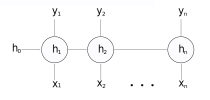
\includegraphics[width=0.5\textwidth]{pics/rnn_network}
  \caption{RNN for NER}
  \label{fig:rnn_network}
\end{figure}

At each timestep, the neural network computes a hidden state $ h_t $ using an input 
vector $ x_t $ and the previous hidden 
state $ h_{t-1} $, that retains information from past 
iterations. The input vector $ x_t $ for the \gls{rnn} could consist, for example, of 
word features indicating if the word is an honorific, if it is the word "that", if it is
capitalized, etc. However, pretrained word embeddings usually provide 
better input vectors for language related tasks, as we will discuss in Section~\ref{ssec:word_embeddings}.
Finally, the \gls{rnn} produces an output vector $ y_t $ representing the label for that 
timestep. A common definition for an \gls{rnn} cell is given by the equations:
\begin{align*}
h_t &= tanh(W_x x_t + W_h h_{t-1}) \\
y_t &= softmax(W_y h_t)
\end{align*}
where $ W_x $, $ W_h $ and $ W_y $ are weight matrices that can be trained with the 
Backpropagation Through Time (BPTT) algorithm~\citep{Werbos1990}. On a sequence labeling task, $ W_y $ 
is a $ |H| \times |Y| $ weight matrix where $ H $ is the size of the hidden layer,
defined experimentally according to the task, and $ Y $ is the number of classification labels
for our problem. With the Softmax activation, the RNN will generate a probability distribution
across the range of possible labels and we can simply select the most probable label at each
timestep, assuming independence between labels. Theoretically, RNNs are capable of learning
and retaining long term dependencies with their internal state $ h_t $. However, in practice,
it becomes difficult due to the vanishing gradient problem~\citep{Bengio1994}, as we will
now discuss. 

The vanishing/exploding gradient problem is one example of an empirical problem that 
constrains theoretically sound network designs. When training neural networks, the weight 
updates are obtained from the partial derivatives of a loss function.
As these derivatives are propagated with the chain rule to distant layers, 
their values tend to get vanishingly small or explode exponentially, what makes training 
less effective. 
This problem is particularly critical for RNNs, because there is the
need to propagate weights over a substantial number of timesteps.
LSTMs were created by~\cite{Hochreiter1997} with this problem in mind and they have been 
popularized because of their effectiveness. LSTMs incorporate a long term memory cell in the form of
a vector $ c $ in addition to the hidden state already present in the conventional RNN. 
This new memory is preserved or updated conditionally based on the observed input. 
A generic description of this architecture is given in Figure~\ref{fig:lstm_partial}.

\begin{figure}[h]
  \centering
  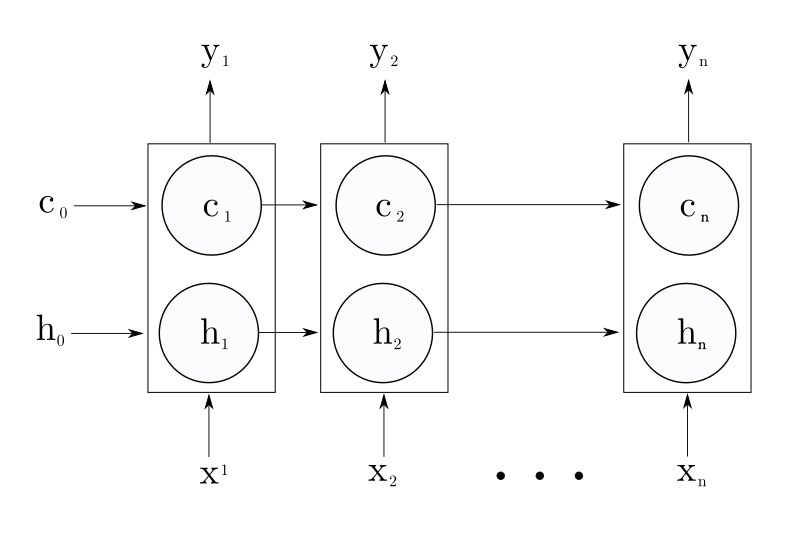
\includegraphics[width=0.5\textwidth]{pics/lstm_partial}
  \caption{RNN with a long term memory cell $ c $.}
  \label{fig:lstm_partial}
\end{figure}

The LSTM has three gates to control the flow of information that comes in and out of the memory
cell $ c $.
The input gate $ \Gamma_{i} $ controls the amount of new information that will flow into the memory cell,
the forget gate $ \Gamma_{f} $ controls the amount of previous information that will be retained in the memory
cell (despite the misleading name), and the output gate $ \Gamma_{o} $ controls the amount of information 
stored in the memory cell that
will be used to compute the output activation of the LSTM unit. 
LSTM implementations vary slightly in the literature. A visual description of 
our LSTM unit is provided in Figure~\ref{fig:lstm_cell}.

\begin{figure}[h]
  \centering
  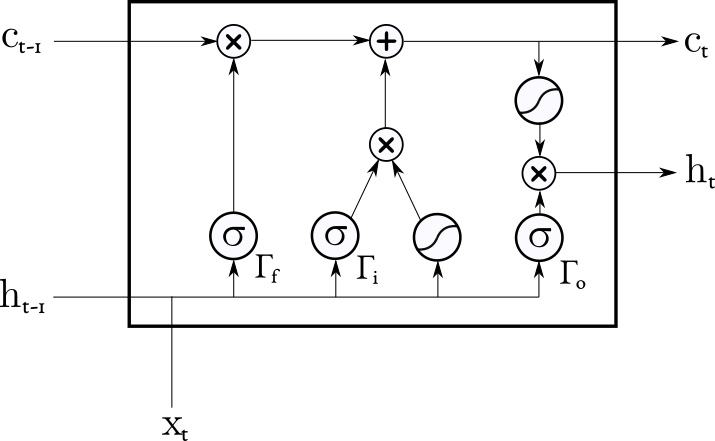
\includegraphics[width=0.5\textwidth]{pics/lstm_cell}
  \caption{LSTM Cell}
  \label{fig:lstm_cell}
\end{figure}

Consider that the vector $ [x_{t},h_{t-1}] $ is formed by concatenating 
the current input vector $ x_{t} $ and the hidden vector from a previous timestep 
$ h_{t-1} $. Also, consider that $ \ast $ represents the Hadamard Product 
(element-wise multiplication) of two matrices with the same dimensions. That is:
%
\begin{equation*}
\begin{bmatrix}
    a_{11} & a_{12} \\
    a_{21} & a_{22} \\
\end{bmatrix} 
\ast
\begin{bmatrix}
    b_{11} & b_{12} \\
    b_{21} & b_{22} \\
\end{bmatrix} 
=
\begin{bmatrix}
    a_{11}b_{11} & a_{12}b_{12} \\
    a_{21}b_{21} & a_{22}b_{22} \\
\end{bmatrix}
\end{equation*}
%
Then, the equations for the LSTM unit are:
%
\begin{align*}
\Gamma_{i} &= \sigma(W_i \cdot [x_t,h_{t-1}] + b_i) \\
\Gamma_{f} &= \sigma(W_f \cdot [x_t,h_{t-1}] + b_f) \\ 
\Gamma_{o} &= \sigma(W_o \cdot [x_{t},h_{t-1}] + b_o) \\
c_t        &= \Gamma_{f} \ast c_{t-1} + \Gamma_{i} \ast tanh(W_c \cdot [x_{t},h_{t-1}] + b_c) \\
h_t        &= \Gamma_{o} \ast tanh(c_t)
\end{align*}
%
where $ \sigma $ is the logistic sigmoid function. $ \Gamma_i $, $ \Gamma_f $, and $ \Gamma_o $ are the input,
forget and output gates, respectively, and $ W_i $, $ W_f $, $ W_o $ are the weight 
matrices corresponding to each gate. $ c_{t} $ is the cell 
state at time $ t $ and $ h_{t} $ is the hidden state at time $ t $. 


\subsection{BI-LSTM-CRF}
\label{ssec:lstm_crf}

On \gls{ner} tasks, knowing both past and future words could be important 
to attribute a label at time $ t $~\footnote{
The timesteps in the context of \gls{lstm}s for sequence labeling refer to positions in
a sequence. So future words are words that come later in the sequence and past words are
words that happen earlier in the sequence.
}. For example, in the sentences "Summer Smith is a lawyer" 
and "Summer came early this year", at the first timestep, it might be useful to know the words
after Summer to correctly label the sequences. When
jointly decoding label sequences with the Viterbi algorithm in \gls{hmm}s or \gls{crf}s,
these codependencies are taken into account, however a regular LSTM network only takes 
past hidden states into consideration. 

A bidirectional LSTM solves this problem by stacking 
two regular LSTMs, and feeding them with observations in opposite directions. The first LSTM 
receives forward states and the second LSTM receives backward states. The hidden states from both 
networks can then be concatenated at each timestep to produce output labels. With this 
architecture, LSTM units may use information from past and future timesteps to decide 
the label at time $ t $. However, labels are still decoded individually at each timestep, because
we are looking at past and future information encoded in the LSTM state but not the actual label
predictions.

\cite{Huang2015} proposed a bidirectional LSTM with a CRF\footnote{
The definition for the Linear-Chain Conditional Random Fields (CRF) layer was given in
Section~\ref{sec:crf}.
} layer (BI-LSTM-CRF) on the output to overcome this obstacle. 
The main benefit of adding a CRF layer 
in the neural sequence model is that the labels are jointly decoded for a whole sentence 
instead of being predicted individually. Some predicted labels should be highly correlated 
in a \gls{ner} task (e.g. I-PER is very likely to happen after B-PER), 
so it is desirable to predict sequences conjointly.
The BI-LSTM-CRF is described in Figure~\ref{fig:bi_lstm_crf}.

\begin{figure}[h]
  \centering
  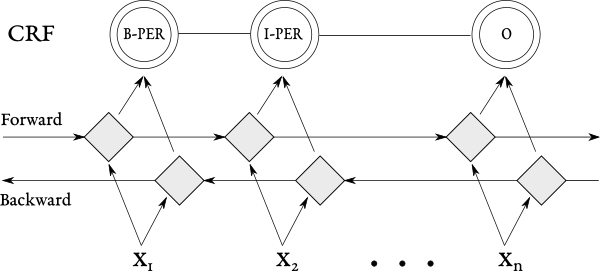
\includegraphics[width=0.5\textwidth]{pics/bi_lstm_crf}
  \caption{Bidirectional LSTM-CRF}
  \label{fig:bi_lstm_crf}
\end{figure}


\subsection{Word Embeddings}
\label{ssec:word_embeddings}

In language-related tasks such as sequence labeling, training data is usually scarce. Because
of the huge number of word combinations that may occur in natural language, most 
combinations will never be observed in the training data. For this reason, it is useful to know 
to which extent two words are related. For example, if the sentence "John is a person" occurs
multiple times in the training data, but the sentence "Joe is a person" never occurs, it may
be useful to know that the words "John" and "Joe" are somewhat related when predicting labels
for this new sentence. This is one of the motivations for using word embeddings as input
vectors for the recurrent neural network architectures presented earlier in this chapter. 

Word embeddings are lower-dimensional representations of words in
continuous space. That is, each word is represented by a vector of continuous features,
typically 50 to 300 dimensions, containing \textit{Ad Hoc} variables whose values are
determined with unsupervised clustering methods for words in large corpora. 
Word embeddings are lower-dimensional in
comparison with the size of the vocabulary, which usually consists of a few hundred thousand words. If we were to use 
binary features to signal the occurrence of a word (one-hot vectors), we would need one feature for each word,
making network training ineffective and the comparison of similarity between different words impossible.
With word embeddings, the number of parameters in the sequence model is dramatically reduced.
Also, the mapping of words into feature vectors makes possible the comparison of 
different words according to their shared features (usually using cosine similarity). And lastly, word embeddings 
can be pre-trained without supervision on large corpora and be used on tasks for which there is 
little labeled data. 

Pre-trained word embeddings are a powerful form of transfer learning. Transfer learning is a group of techniques concerned 
with bootstrapping the learning of model parameters by obtaining information from another dataset not directly
related to the problem. This is especially useful in \gls{ner}, because named entities that 
belong to the same class tend to have similar word embeddings. Thus, with good word embeddings, 
a neural network might predict the correct label for a word that was never seen during training
because this label is similar to other words that occurred in the training set.

There are multiple methods to produce word embeddings, and most of the official implementations 
also provide pre-trained word embeddings for the English language. In this work, we explored
three sets of pre-trained embeddings: Word2Vec~\citep{Mikolov2013}, GloVe~\citep{Pennington2014} and 
ELMo~\citep{Peters2018}. The characteristics of each set of embeddings is given in 
Table~\ref{tab:word_embeddings}.

\begin{table}[h]
  \small
  \begin{center}
    \begin{tabular}{ lllll }
      \toprule
      Model & Dimensions & Training Set & Tokens (billions) & Vocab. \\
      \midrule
      Word2Vec & 300 & Google News & 100 & 3M   \\
      GloVe    & 300 & Gigaword5 + Wikipedia & 42 & 400K \\
      ELMo     & 512 & Wikipedia & 5.5 & - \\
      \bottomrule
    \end{tabular}
  \end{center}
  \caption{Statistics of pre-trained word embeddings.}
  \label{tab:word_embeddings}
\end{table}

Most breakthroughs in sequence labeling in the past few years came with the introduction
of novel methods for constructing word embeddings, as was the case for the three methods mentioned earlier. 
Different from earlier methods such as Word2Vec and
GloVe that produced static vectorial representations of words, more recent approaches such as
ELMo produce context dependent embeddings for a specific dataset with a neural network 
pre-trained on a language modelling task. Also, the word representations in ELMo are entirely character based,
therefore there are no out-of-vocabulary words.


\subsection{Character Representations}
\label{ssec:char_representations}

When creating deep neural architectures, one of the objectives is to allow the 
neural network to discover useful features by itself instead of feeding it with what
we think is relevant. In NER, morphological features are very useful to classify
named entities. For example, knowing that a word ends in "ing" means that it is probably
a verb and therefore it is unlikely to be a proper name. We can add a character 
representation layer at the bottom of the Bi-LSTM-CRF to extract these morphological
features automatically. The character representations, which are fixed size vectors
that encode morphological features, are concatenated to word embeddings and fed to
the \gls{lstm}.

In the next Subsection, we describe two methods to build character representations. Both of them receive 
character embeddings as inputs. Character embeddings are fixed size dense vectors that work
the same way as word embeddings, except that the lookup function maps characters to embeddings
instead of words to embeddings. This means that each word generates a character embedding 
matrix with size $ |W| \times |C| $, where $ |W| $ is the word length and $ |C| $ is the 
character embedding size (determined experimentally). Also, the character embeddings are 
trained directly in the target dataset, since the vocabulary size is much smaller than in 
the case of word embeddings.


\subsubsection{CNN character representations}
\label{sssec:lstm_crf_cnn}

The \gls{cnn} method proposed by~\cite{Ma2016} uses a \gls{cnn} layer 
at the bottom of the Bi-LSTM-CRF architecture to encode character-level 
information. The \gls{cnn} layer is described visually in Figure~\ref{fig:cnn}.
%
\begin{figure}[h]
  \centering
	  \includegraphics[width=0.5\textwidth]{pics/cnn}
  \caption{CNN-based character representations for the word "jaguar".}
  \label{fig:cnn}
\end{figure}
%
The \gls{cnn} receives character embeddings as inputs. For example, if the character
embeddings have 50 dimensions, then the input matrix representing word "jaguar" would be 
a $ 50 \times 6 $ matrix. The one dimensional convolution operation works by sliding
fixed size kernels over the input matrix producing scalar values at each position. These
kernels, also called filters, try to detect morphological patterns in the 
input matrix such as "ing" or "son". In this example, we define three kernels with window
size 3 (which is usually a good number for detecting useful prefixes and suffixes), each
kernel consists of a $ 50 \times 3 $ matrix. At each window position in the
word (i.e. "jag", "agu", "gua" and "uar"), we perform a convolution
over each of the 50 channels (character embedding features) adding up the results 
to produce a scalar value. This way, after running the three kernels over the input 
matrix, we get a $ 4 \times 3 $ matrix indicating at each window position the extent to which
each filter was activated. Finally, we perform a global max pooling operation that collapses
the filter dimension taking its maximum value over the 4 window positions, producing a 
vector with 3 dimensions that indicates for each filter, if it was triggered in that word.
This means, that when a filter gets a good match at any position in the sequence, the 
max pooling layer output relative to that filter will be triggered, therefore this type of 
character representation detects position invariant morphological features. For example,
the word "finger" would trigger a filter for "ing" the same way the word "writing" would
trigger this filter. 

\subsubsection{LSTM character representations}

The LSTM method proposed by~\cite{Lample2016} models character-level 
representations with a Bi-LSTM similar to the one described in 
Figure~\ref{fig:bi_lstm_crf}, however instead of receiving words as inputs, it receives
sequences of character embeddings. Also, instead of producing an output at each timestep,
we are only interested in obtained the hidden state at the first timestep for the backward
LSTM and the hidden state for the last timestep for the forward LSTM. The combined forward 
and backward states are concatenated to form the character representation, as described visually
in Figure~\ref{fig:lstm_char}. 

\begin{figure}[h]
  \centering
  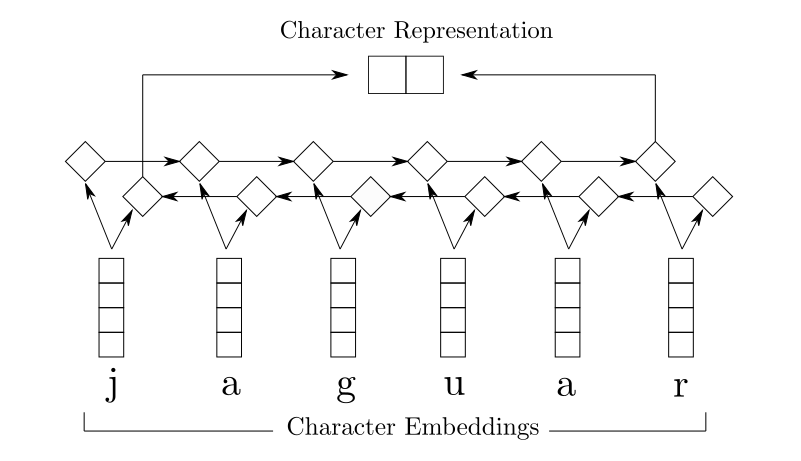
\includegraphics[width=0.5\textwidth]{pics/lstm_char_representations}
  \caption{LSTM-based character representations for the word "jaguar".}
  \label{fig:lstm_char}
\end{figure}

The forward state is expected to be a better representation of the suffix of 
a token, and the backward state is expected to be a better representation of 
the prefix of a token. This differentiates the architecture
from the \gls{cnn} method, because the \gls{lstm} based representations are 
not positional invariant.


\chapter{Researcher Name Extraction Dataset}
\label{cha:dataset}

%%% @ Review 5
%%% Explain why the dataset is valid.

This chapter describes the dataset used to evaluate the performance of sequence labeling models
on the task of \gls{rne}. We call it the \gls{rne} dataset.
We attested experimentally that 
models trained in a popular \gls{ner} dataset (the {CoNLL-2003} English dataset) do not perform 
well in the \gls{rne} task and this is likely due to the differences
between plain text and HTML. The lack of other \gls{ner} 
datasets built for HTML name extraction imposes the need to construct a dataset specific for \gls{rne}.

The \gls{rne} task consists of finding researcher names in faculty listings from university 
webpages across the world, mainly from Computer Science departments.
This would be a necessary step when linking researcher profiles from university 
websites to their entries in public databases. Unlike many
\gls{wde} datasets, each webpage in the \gls{rne} dataset comes from a different 
website, and therefore has a different format, what makes many \gls{wde}
approaches impractical. The idea is to explore systems that are general 
enough to allow accurate entity extraction from different sources while requiring
no supervision between different websites. 

We collected 145 Computer Science and Engineering faculty pages from 42 different countries in
multiple languages, although the English version was favored whenever it was available.
We gathered faculty webpages in proportion to
the number of universities in each country\footnote{A detailed list of universities can
be found in https://univ.cc/world.php}. 
The dataset size was limited to a number of pages that could be viably labeled manually and
that could still represent many different countries. 
Also, university pages that contained 
corrupt HTML or JavaScript code that performed lazy loading of data records were
not included in this dataset.

This chapter is divided as follows. Section~\ref{sec:data_description} describes the 
dataset format and how it was split in
three data files. 
Section~\ref{sec:evaluation} describes how the evaluation of results in this 
dataset was carried on. 
Section~\ref{sec:dictionary} describes how we obtained a dictionary
of relevant named entities for this dataset, and discusses some baselines.
Lastly,
Section~\ref{sec:conll_comparison} compares the characteristics of the \gls{rne} dataset
with another popular \gls{ner} dataset, the {CoNLL-2003} English \gls{ner} dataset.

\section{Data Description} 
\label{sec:data_description}

Each of the 145 faculty pages was preprocessed and converted
to the {CoNLL-2003} data format. That is, one word per line with empty lines representing
sentence boundaries. Sentence boundaries were determined by line break HTML tags
(div, p, table, li, br, etc.) in contrast to inline tags (span, em, a, td, etc.). For example,
the HTML sentence: 
%
\begin{quote}
\centering
<p>E. <b>Smith</b> is a <a href="/link">professor</a>.</p>
\end{quote}
%
\noindent
becomes:
%
\begin{quote}
\centering
E. Smith is a professor.
\end{quote}
%
Sentences that were more than fifty tokens long were also split according to the
punctuation. Some algorithms have trouble handling very big sentences, so we verified
experimentally that fifty tokens provide a large enough context 
and allow efficient training using a GPU. A few sentences in the dataset would be 
more than a thousand tokens long if this step was not performed, what would make batch training
for neural networks less efficient.

% The algorithm used for sentence segmentation is described in
% Appendix~\ref{app:html_segmenter}.

A robust tool for HTML segmentation poses many challenges by itself, but the simple approach 
adopted here has proved to be sufficient to perform \gls{rne} adequately. 
Also, it is best to evaluate \gls{ner} models without relying on any sophisticated data 
record segmentation system.
In many cases, entity annotation may precede the segmentation
phase on \gls{wde} methods. Also, depending on the task (as is the case
for researcher name extraction), a good annotator that is able to work 
with raw HTML provides a good solution to the problem.

Finally, all tokens were tagged using the IOB scheme put forward by~\cite{Ramshaw1999}
and used in {CoNLL-2003}, this is:

\begin{quote}
Words tagged with O are outside of named entities
and the I-XXX tag is used for words inside a
named entity of type XXX. Whenever two entities of
type XXX are immediately next to each other, the
first word of the second entity will be tagged B-XXX
in order to show that it starts another entity~\citep{KimSang2003}.
\end{quote}

The \gls{rne} dataset only has entities of type person PER, therefore a classifier has to
label each token with one of the labels: O, B-PER, or I-PER. The following example 
sentence, obtained from the dataset, illustrates proper token labeling:

\begin{table}[h]
  \small
  \begin{center}
    \begin{tabular}{ ll }
      Token & Correct Label \\
      \midrule
      Kasper    & I-PER \\ 
      Rasmussen & I-PER \\
      Associate & O     \\
      Professor & O     \\    
      ,         & O     \\    
      Royal     & O     \\    
      Society   & O     \\    
      Research  & O     \\    
      Fellow    & O     \\    
    \end{tabular}     
  \end{center}
\end{table}

The \gls{rne} dataset was divided in a training, a validation and a test set, as described in 
Table~\ref{tab:dataset}. The sizes of the data files were divided in approximately
the same proportion adopted in other sequence labeling datasets such
as {CoNLL-2003}, that is described in Table~\ref{tab:conll}. Only the training set was used
to fit model parameters. Models that relied on numerical optimization methods such as 
neural networks were evaluated successively on the validation set during training to avoid overfitting. 
That is, the validation set was never observed during training, but it provided an unbiased 
evaluation of model performance. We kept training parameters until the performance in the 
validation set no longer improved. This is called the early stopping validation strategy.
The comparison of different models was conducted by comparing their performance in the test set, 
which is never observed during training or used in the validation strategy.

\begin{table}[h]
  \small
  \begin{center}
    \begin{tabular}{ lllll }
      \toprule
      Data file & Documents & Sentences & Tokens & Names \\
      \midrule
      Training    & 85  & 24,728 & 110,269 & 5,822  \\  
      Validation  & 30  & 8,743  & 36,757  & 1,788  \\
      Test        & 30  & 10,399 & 44,795  & 2,723  \\
      \midrule
      Total       & 145 & 43,870 & 151,821 & 10,333 \\
      \bottomrule
    \end{tabular}
  \end{center}
  \caption{Description of the data files in the RNE dataset.}
  \label{tab:dataset}
\end{table}

\begin{table}[h]
  \small
  \begin{center}
    \begin{tabular}{ llllllll }
      \toprule
      Data file & Documents & Sentences & Tokens & LOC & MISC & ORG & PER \\
      \midrule
      Training    & 946  & 14,987 & 203,621 & 7,140 & 3,438 & 6,321 & 6,600 \\  
      Validation  & 216  & 3,466  & 51,362 & 1,837 & 922 & 1,341 & 1,842  \\
      Test        & 231  & 3,684  & 46,435 & 1,668 & 702 & 1,661 & 1,617  \\
      \midrule
      Total       & 1,393 & 22,137 & 301,418 & 10,645 & 5,062 & 9,323 & 10,059 \\
      \bottomrule
    \end{tabular}
  \end{center}
  \caption{Description of the {CoNLL-2003} English dataset}
  \label{tab:conll}
\end{table}


Most webpages in this dataset are faculty directories with informative
text in small passages, even if long prose is not absent. 
Size and structure varies wildly, therefore some documents 
may contain up to a few hundred names whereas other documents may contain 
only a dozen names. This difference in document size and characteristics 
may be problematic when comparing different extraction systems, because a system 
that performs well on some types of pages may perform poorly on other types.
To avoid this problem, we tried to keep the proportion between the number of tokens
and the number of documents roughly the same for all data files.

\section{Evaluation}
\label{sec:evaluation}

The performance of classifiers in the \gls{rne} dataset was evaluated according to their precision (P), recall (R) and F-scores
in the test set. The precision and recall 
measures are defined in terms of the number of true positives, false negatives, and false 
positives made by the classifier when extracting named entities. That is:

\begin{equation*}
\text{Precision} = \frac{\text{TruePos}}{\text{TruePos} + \text{FalsePos}}      
\qquad
\text{Recall} = \frac{\text{TruePos}}{\text{TruePos} + \text{FalseNeg}}
\end{equation*}

Precision accounts for the proportion of named entities found by the model that are 
correct relative to all predicted named entities.
Recall is the proportion of named entities correctly predicted by the model relative to
all named entities in the dataset. Precision measures Type I errors 
(false positives) and recall measures Type II errors (false negatives). Partial matches are
not considered, so a classification only counts as a true positive if the entire named entity
has been correctly extracted. Additionally, the F-score, proposed by~\cite{Rijsbergen1979}, 
is a composite measure that combines precision and recall, defined as:

\begin{equation}
F_{\beta} = (1 + \beta^2) \cdot \frac{\text{Precision} \cdot \text{Recall}}{(\beta^2 \cdot \text{Precision}) + \text{Recall}}
\label{eq:fscore_formula}
\end{equation}

The choice of $ \beta $ depends on the relative importance attributed to precision over recall.
This formula ``measures the effectiveness of retrieval with respect to a user who attaches 
$ \beta$ times as much importance to recall as precision''~\citep{Rijsbergen1979}. A common choice
for the value of $ \beta $ is $ 1 $, in which case the measure is called the $ F_1 $-score (F1). 
Whenever the $F_1$-score is used, we attribute 
as much importance to recall as to precision.

In our experiments, we measured the precision, recall and $ F_1 $-scores over the entire 
data files. Considering that each webpage has a different number of named entities,
this naturally privileges models that work well for pages with more named entities. 
A different approach might be to consider the averaged precision, recall and $ F_1 $-scores 
per webpage, privileging systems that have more regularity between different websites. However, 
this approach would also have negative implications. That is, the impact of errors in pages with many 
named entities would diminish and the impact of errors in pages with few named entities would
increase. So, the former approach was preferred.


\section{Dictionary}
\label{sec:dictionary}

%%% @ Review 6
%%% Recalculate stats for each datafile and show results for the dictionary 
%%% matching approach. Show results for the 3 models over the entire dataset.

A dictionary of named entities can be a powerful aid to sequence labeling systems,
especially when considering traditional statistical methods. For the \gls{rne} task, we extracted 
a list of 1,595,771 researcher names from the DBLP database and annotated tokens in the
\gls{rne} dataset with exact and partial match tags. That is, if a sequence of tokens
corresponded exactly to a name from the DBLP list, the entire sequence was annotated as 
an exact match. Otherwise, if only some tokens in the sequence matched a name from the DBLP
list partially, the matching tokens were annotated with a partial match tag. This dictionary
was used by some of the models that will be discussed in the experiments chapter, however it 
must be stated that one of the main advantages of Deep Neural Networks relative to other
approaches is the fact that they can perform well even without the aid of a dictionary.

\begin{table}[h]
  \small
  \begin{center}
    \begin{tabular}{ lllll }
      \toprule
      Data file & Precision & Recall & F1 & Correct names \\
      \midrule
      Training   & 0.7316 & 0.2303 & 0.3504 & 1,341 of 5,822 \\ 
      Validation & 0.8474 & 0.2858 & 0.4274 & 511 of 1,788 \\ 
      Test       & 0.8717 & 0.3268 & 0.4754 & 890 of 2,723 \\ 
      \bottomrule
    \end{tabular}
  \end{center}
  \caption{
    DBLP dictionary coverage in each data file of the RNE dataset, when an 
    exact dictionary matching strategy is used.
  }
  \label{tab:gazetteer}
\end{table}

To understand how this dictionary can be useful for some models in the \gls{rne}, 
we measured the precision, recall and $ F_1 $-scores for an exact dictionary matching 
strategy in each \gls{rne} data file. The results, shown in 
Table~\ref{tab:gazetteer}, provide a baseline with which to compare
other methods of sequence labeling. 
Any useful extraction method should at least improve upon this approach.
Recall is very low because the dictionary is incomplete and precision falls short of
top performing extraction methods. This last result is surprising since we are only extracting 
exact matches. The reason for the low precision is that exact dictionary matches may actually 
only correspond to partial matches in the dataset. For example, if the dictionary has an entry
for "Ann Smith", it may partially overlap an entry in the dataset for "Mary Ann Smith", yielding
a false positive.


\section{Comparison with {CoNLL-2003}}
\label{sec:conll_comparison}

The {CoNLL-2003} dataset was introduced in the \gls{ner}
shared-task in 2003 and is frequently used to attest 
the performance of state-of-the-art sequence labeling systems~\citep{Huang2015,Lample2016,Ma2016,Peters2018}. 
The English data, which is composed of news stories extracted from the Reuters Corpus, 
provides annotations for four types of entities: people (PER), organizations (ORG), 
locations (LOC), and miscellaneous (MISC), i.e., entities that cannot be 
classified in one of the former groups. The statistics for the {CoNLL-2003} dataset 
were already described in Table~\ref{tab:conll}.

If the {CoNLL-2003} English dataset is used to both train and evaluate 
state-of-the-art models, it is to be expected that models trained in this dataset will
be able to extract the same named entities in other documents with reasonable 
effectiveness. However, this is hardly the case. This is because tabular HTML 
documents, such as faculty listings, are very different from plain text. Using our
labeled dataset for \gls{ner} on HTML, we can understand how different news stories written 
in free text format and faculty listings in HTML format really are.

We trained three classifiers to perform the task of person name extraction using
the {CoNLL-2003} training set. The {CoNLL-2003} dataset was relabeled so that classifiers only had to extract
person entities (PER labels), thus other entity types (LOC, ORG, and MISC) were relabeled as
not an entity (O label). Next, we trained the classifiers with the relabeled {CoNLL-2003} training set,
and validated the results with the relabeled validation set. The models were tested with the relabeled {CoNLL-2003}
test set and the \gls{rne} test set.
In Table~\ref{tab:conll_to_ner_on_html}, we present the results for a first order \gls{hmm}, 
a Linear Chain \gls{crf}, and a Bi-LSTM-CRF classifier with GloVe embeddings~\citep{Huang2015} in the 
aforementioned experimental setting.

\begin{table}[h]
  \small
  \begin{center}
    \begin{tabular}{ lllllll }
      \toprule
      \multirow{2}{*}{Model} & \multicolumn{3}{c}{CoNLL-2003} & \multicolumn{3}{c}{\gls{rne}} \\
                             & \multicolumn{1}{c}{P} & \multicolumn{1}{c}{R} & \multicolumn{1}{c}{F1}
                             & \multicolumn{1}{c}{P} & \multicolumn{1}{c}{R} & \multicolumn{1}{c}{F1} \\
      \midrule
      HMM         & 0.777 & 0.452 & 0.571\ \ \ & \ \ \ 0.189 & 0.180 & 0.184 \\
      CRF         & 0.774 & 0.754 & 0.764\ \ \ & \ \ \ 0.138 & 0.129 & 0.133 \\
      Bi-LSTM-CRF & 0.969 & 0.931 & 0.950\ \ \ & \ \ \ 0.282 & 0.258 & 0.269 \\
      \bottomrule
    \end{tabular}
  \end{center}
  \caption{
    Performance of three classifiers trained with the {CoNLL-2003} training set and tested in
    the CoNLL-2003 and RNE test sets.
  }
  \label{tab:conll_to_ner_on_html}
\end{table}

The very low $ F_1 $-score obtained by all models on the \gls{rne} test set is much lower and even worse 
than the established dictionary baseline in Table~\ref{tab:gazetteer}. We cannot use these results to 
properly compare the relative performances 
between the models (this topic will be explored in the next chapter), but it is possible to conclude
that machine learning models trained on plain text do not necessarily perform well in HTML 
extraction tasks. The Bi-LSTM-CRF model obtained a 0.269 $ F_1 $-score in the \gls{rne} test
set, what is surprising considering that it is a very efficient approach to sequence labeling in plain 
text. By looking at some of its mistakes we can shed some light on this result. The Bi-LSTM-CRF model
extracted "Dean Emeritus" and "14101 INF" as names, and it missed the last names in "George E. Elliott"
and "Carl J. Galligan". These mistakes are representative of some of the major flaws with the systems
trained with the CoNLL-2003 training set. The names in the \gls{rne} dataset 
are usually longer than in CoNLL-2003 and the word distributions are vastly different, what may
account for some of the mistakes of the Bi-LSTM-CRF model.

Let us examine some differences between both datasets. 
The number of documents in the \gls{rne} dataset is 145, which is much smaller than
the 1,393 documents in the ConLL-2003 dataset. However, the number of sentences in the \gls{rne}
dataset is higher, that is 43,870 sentences against 22,137 in the ConLL-2003 dataset. Also, the number 
of tokens in the \gls{rne} dataset
is roughly half the number present in the {CoNLL-2003} dataset. These numbers show that 
the HTML documents in the \gls{rne} dataset are longer than news 
stories and, more importantly, they are composed of much shorter sentences when compared 
to the text from news corpora. Indeed, there are 3.46 words per sentence in the \gls{rne} dataset
against 13.62 words per sentence in the {CoNLL-2003} dataset. Most faculty webpages have a lot of 
boilerplate text that contributes to their size, while the news stories in {CoNLL-2003}
are usually rather short. These numbers show that HTML provides far less context to named entity recognition
by sequence models. One key implication is that any good classifier needs to seek other sources of 
evidence in addition to the text, such as dictionaries and the HTML structure.

Another property that is quite distinct among different NER datasets is their word distributions. Word frequencies
tend to vary considerably in documents with different topics. Table~\ref{tab:frequent_words}
shows the ten most frequent words for each dataset, including punctuation signs. Punctuation
signs are frequently present in proper names, as in: Mary B. Smith, Susan (Susie) Williams, John Al-Azzawi, etc.
Also, punctuation signs can be useful to detect boundaries between named entities.
The {CoNLL-2003} English dataset contains a more generic selection of terms whereas the 
subject of the \gls{rne} dataset becomes evident with words such as "professor" and "university" 
happening with a high frequency in the corpus. Also, punctuation signs are much more frequent in
the \gls{rne} dataset. 

Lastly, in Figure~\ref{fig:word_frequency_plot}
we plot the word frequencies for the hundred most frequent words in the {CoNLL-2003} and 
the \gls{rne} datasets. In both plots we have a few very frequent words and a long tail of
infrequent words. Most named entities are located in this long tail, and therefore, a good sequence
labeling method needs to be able to handle the labeling of infrequent tokens effectively. 
The probabilities attributed to unseen tokens is another aspect where models vary significantly 
between different datasets.


\begin{table}[h]
  \small
  \begin{center}
    \begin{tabular}{ llll }
      \toprule
      \multicolumn{2}{c}{CoNLL-2003} & \multicolumn{2}{c}{\gls{rne}} \\
      \multicolumn{1}{c}{Word} & \multicolumn{1}{c}{Frequency} &
      \multicolumn{1}{c}{Word} & \multicolumn{1}{c}{Frequency} \\
      \midrule
      the & 12310 & , & 10439      \\
      , & 10876 & - & 8140         \\
      . & 10874 & ) & 3655         \\
      of & 5502 & ( & 3641         \\
      in & 5405 & : & 3484         \\
      to & 5129 & of & 3345        \\
      a & 4731 & and & 2499        \\
      ( & 4226 & professor & 2456  \\
      ) & 4225 & university & 1611 \\
      and & 4223 & research & 1315 \\
      \bottomrule
    \end{tabular}
  \end{center}
  \caption{Ten most frequent words for the {CoNLL-2003} and the RNE datasets.}
  \label{tab:frequent_words}
\end{table}

\begin{figure}[h!]
  \begin{center}
    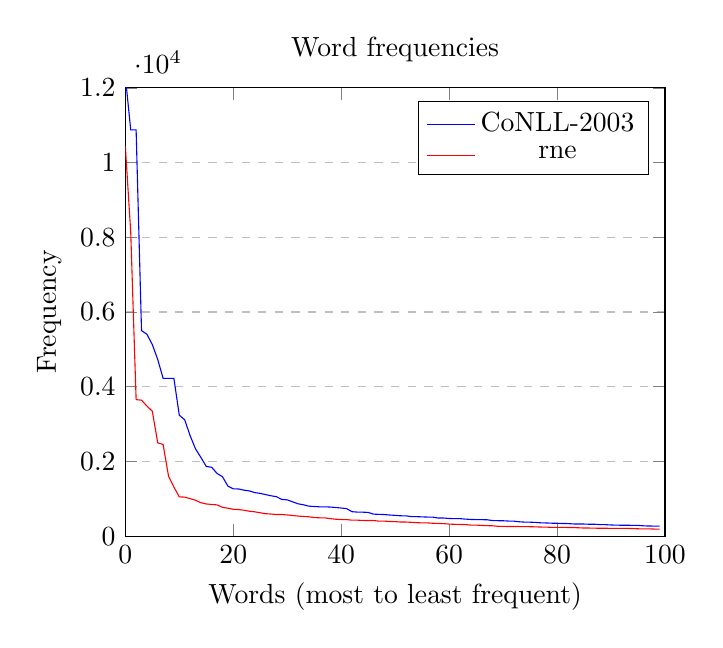
\begin{tikzpicture}
      \begin{axis}[
        title={Word frequencies},
        xmin=0, xmax=100,
        ymin=0, ymax=12000,
        ylabel={Frequency},
        xlabel={Words (most to least frequent)},
        ymajorgrids=true,
        grid style=dashed,
        legend pos=north east,
        % scaled y ticks=false,
      ]

      \addplot[color=blue, color=blue] coordinates {
        (0,12310)(1,10876)(2,10874)(3,5502)(4,5405)(5,5129)(6,4731)(7,4226)(8,4225)(9,4223)(10,3239)(11,3115)(12,2694)(13,2339)(14,2109)(15,1866)(16,1845)(17,1679)(18,1593)(19,1342)(20,1267)(21,1264)(22,1232)(23,1212)(24,1166)(25,1146)(26,1113)(27,1082)(28,1057)(29,984)(30,973)(31,920)(32,867)(33,841)(34,804)(35,796)(36,786)(37,786)(38,780)(39,768)(40,754)(41,738)(42,656)(43,645)(44,643)(45,636)(46,591)(47,584)(48,579)(49,567)(50,558)(51,546)(52,545)(53,524)(54,523)(55,517)(56,512)(57,510)(58,486)(59,486)(60,474)(61,470)(62,470)(63,457)(64,448)(65,444)(66,442)(67,441)(68,419)(69,415)(70,413)(71,405)(72,402)(73,386)(74,377)(75,375)(76,369)(77,358)(78,354)(79,348)(80,346)(81,340)(82,338)(83,328)(84,327)(85,325)(86,320)(87,319)(88,310)(89,308)(90,300)(91,296)(92,293)(93,292)(94,291)(95,289)(96,278)(97,272)(98,271)(99,271)
      };
      \addplot[color=red, color=red] coordinates {
        (0,10439)(1,8140)(2,3655)(3,3641)(4,3484)(5,3345)(6,2499)(7,2456)(8,1611)(9,1315)(10,1053)(11,1046)(12,1006)(13,963)(14,897)(15,863)(16,849)(17,838)(18,773)(19,749)(20,720)(21,713)(22,695)(23,668)(24,652)(25,626)(26,602)(27,593)(28,581)(29,580)(30,569)(31,553)(32,539)(33,527)(34,520)(35,499)(36,492)(37,490)(38,469)(39,454)(40,446)(41,444)(42,429)(43,429)(44,422)(45,420)(46,419)(47,403)(48,403)(49,394)(50,390)(51,379)(52,379)(53,371)(54,362)(55,356)(56,355)(57,346)(58,342)(59,337)(60,324)(61,318)(62,314)(63,311)(64,298)(65,297)(66,288)(67,282)(68,279)(69,265)(70,263)(71,259)(72,259)(73,258)(74,258)(75,254)(76,250)(77,245)(78,243)(79,236)(80,236)(81,235)(82,234)(83,232)(84,225)(85,219)(86,218)(87,215)(88,212)(89,212)(90,210)(91,209)(92,208)(93,208)(94,205)(95,198)(96,197)(97,196)(98,191)(99,191)
      };
      \legend{CoNLL-2003, \gls{rne}};
       
      \end{axis}
    \end{tikzpicture}
    \caption{
      Word frequencies plot for the {CoNLL-2003} dataset and the RNE dataset.
    }
    \label{fig:word_frequency_plot}
  \end{center}
\end{figure}


\chapter{Experiments}
\label{cha:experiments}

%%% Review 2 
%%% Change "featureless models" to something else.

The main objective of this dissertation is to find the best methods for performing \gls{ner} on the 
Web considering the \gls{rne} task. The value of a specific method is determined
not only by its accuracy, but also by the amount of feature engineering required, the training
time required, and the overall complexity of the model when we consider its gains relative to
simpler alternatives. With this objective in mind, we pose the following research questions:

\begin{enumerate}

\item How effective are HMMs for solving the RNE task?
\begin{enumerate}
\item Does the order of the HMM influence its performance?
\item Can we improve a HMM by adding textual features?
\item Can we improve a HMM with the self-training strategy?
\end{enumerate}

\item How effective are CRFs for solving the RNE task?
\begin{enumerate}
\item Are CRFs better than HMMs?
\item Can we improve the CRFs by adding textual features?
\item Are CRFs more resilient to bad features than HMMs?
\end{enumerate}

\item How effective are Neural Networks for solving the RNE task?
\begin{enumerate}
\item How does a Bi-LSTM-CRF compare with HMMs and CRFs?
\item Can character representations boost the performance of the Bi-LSTM-CRF?
\item Does the selection of word embeddings influence the performance of the Bi-LSTM-CRF?
\end{enumerate}

\item All things considered what is the best model?
\begin{enumerate}
\item What model has the best F1-score?
\end{enumerate}

\end{enumerate}

All models in this dissertation were trained and tested in the dataset described in Chapter~\ref{cha:dataset}.
When relevant, the technical specifications for the experiments will be given in each section.
Section~\ref{sec:baseline} establishes a baseline in addition to the dictionary
matching baseline that was described in Chapter~\ref{cha:dataset} for the \gls{rne}
task. Section~\ref{sec:experiments_hmm} discusses the experimental results that concern
Research Question 1. Section~\ref{sec:experiments_crf} discusses the experimental results that 
concern Research Question 2. Section~\ref{sec:experiments_nn} discusses the experimental results 
that concern Research Question 3. Finally, Section~\ref{sec:experiments_best} discusses the experimental 
results that concern Research Question 4.


\section{Simple Baseline}
\label{sec:baseline}

%%% @ Review 7
%%% Retrain NB and Maxent with cross validation.

A model that works well despite the absence of a good feature selection is arguably more valuable than
a method that requires a lot of feature engineering or a big dictionary of named entities, as long as 
its accuracy is sufficiently high for the intended purpose.
For this reason, we wanted to establish some baseline results in addition to 
the dictionary matching results presented in Chapter~\ref{cha:dataset}. We
trained a simple generative model and a simple discriminative model to provide a measure of the
expected difficulty of solving this task. The simple generative model is a Naive Bayes classifier,
which is essentially a \gls{hmm}, as presented in Section~\ref{sec:hmm}, with the
only difference being that it assumes label independence. That is, $ P(Y_i|Y_{i-1}) = P(Y_i) $ for all timesteps $ i $. 
The simple discriminative model is a Logistic Classifier, as presented in Section~\ref{sec:crf}. 

The ``Naive-Bayes and Logistic Classifiers form a generative-discriminative pair'', as
explained by~\cite{Ng2001},
in the sense that the essential difference between the models is that the first estimates the
joint probability between words and labels $ P(X, Y) $ and the latter models the conditional
probability $ P(Y|X) $. The same analogy could be made for HMMs and CRFs. The Naive Bayes model and
the Logistic Classifier are very simple and fast to train, so they provide a good 
first approximation to a solution for this task. Both models used only the current word as a
feature. Table~\ref{tab:nb_and_maxent} shows a comparison between these models and the exact dictionary
matching approach\footnote{
That is, using a dictionary of 
researcher names extracted from DBLP, a sequence of tokens was labeled as a name if it corresponded
exactly to an entry in this dictionary. 
} presented in Chapter~\ref{cha:dataset}. We show results for the models in the validation and 
test sets of the \gls{rne} dataset. The difference between the validation and test sets is
only of significance when discussing neural networks, which are trained in the training set 
until the F1-score in the validation set stops improving. For the other models, the data
from the validation and test sets is never observed during training. When comparing different 
models we will always consider results in the test set.


\begin{table}[h]
  \small
  \begin{center}
    \begin{tabular}{ lllllll }
      \toprule
      \multirow{2}{*}{Model} & \multicolumn{3}{c}{Validation} & \multicolumn{3}{c}{Test} \\
                             & \multicolumn{1}{c}{P} & \multicolumn{1}{c}{R} & \multicolumn{1}{c}{F1}
                             & \multicolumn{1}{c}{P} & \multicolumn{1}{c}{R} & \multicolumn{1}{c}{F1} \\
      \midrule
      Dictionary Matching    & 0.847 & 0.285 & 0.427 & 0.871 & 0.328 & 0.477   \\
      Naive Bayes            & 0.068 & 0.053 & 0.059 & 0.101 & 0.075 & 0.086   \\
      Logistic Classifier    & 0.952 & 0.171 & 0.122 & 0.116 & 0.156 & 0.133   \\
      % Logistic             & 0.132 & 0.119 & 0.125 & 0.102 & 0.096 & 0.099   \\
      \bottomrule
    \end{tabular}
  \end{center}
  \caption{Naive Bayes and Logistic Classifier results for the researcher name extraction task
  using only the current word as a feature.}
  \label{tab:nb_and_maxent}
\end{table}

The Logistic Classifier performs a little better than the Naive Bayes model in this problem, 
but both models are rather ineffective. The problem is that these classifiers always assign 
an O tag to unknown tokens~\footnote{
Unknown tokens are tokens that occur at least once in the validation or test sets 
but do not occur in the training set.
}, what is understandable since the proportion of O tags in the dataset 
is approximately 86\% and each token is classified independently. 
Table~\ref{tab:unknown_tokens} shows the number of unknown tokens in the validation and test
sets, and the number of named entities that contain at least one unknown token. Roughly four in 
every five named entities contain at least one unknown token, therefore, a classifier that only
considers the current token as a feature and attributes labels independently can obtain
at best 20\% recall. Also, the proportion of unknown tokens in the validation set is higher
than in the test set, what may account for the drop in performance for both classifiers in the
validation set relative to the test set.

The Naive Bayes and the Logistic Classifier performed significantly worse than the dictionary 
matching approach. These models are not suited for sequence classification problems and
that is why we need approaches such as \gls{hmm}s, \gls{crf}s, and Neural Networks. However,
these baselines provide a very useful insight. That is, the amount of 
probability mass attributed to unknown observations is of great importance to the performance
of \gls{ner} methods.

\begin{table}[h]
  \small
  \begin{center}
    \begin{tabular}{ lllll }
      \toprule
      Tokens / Named Entities (NE) & Valid & \% & Test & \%\\
      \midrule
      Unknown Tokens & 12076 & 26.96\% & 8324  & 22.65\% \\
      Known Tokens   & 32719 & 73.04\% & 28433 & 77.35\% \\
      Total          & 44795 & 100.00\%   & 36757 & 100.00\%   \\
      \midrule
      NEs with Unknown Tokens    & 1446 & 80.87\% & 2205 & 80.98\% \\
      NEs without Unknown Tokens & 342  & 19.13\% & 518  & 19.02\% \\
      Total                      & 1788 & 100.00\% & 2723 & 100.00\%   \\
      \bottomrule
    \end{tabular}
  \end{center}
  \caption{Unknown tokens in the RNE dataset.}
  \label{tab:unknown_tokens}
\end{table}


\section{Hidden Markov Models}
\label{sec:experiments_hmm}

%%% @ Review 8
%%% Retrain HMMs with cross validation.

There are a couple of parameters that need to be considered when we employ Hidden Markov Models
to a sequence labeling task on the Web. First, the number of previous states (the order of the HMM), 
second, the features, and third, the self-training strategy.

\subsection{HMM order}

We hypothesized that the performance of HMMs on sequence labeling tasks for NLP can be improved by
increasing the number of previous states checked at each timestep, i.e., the order of the HMM.
Figure~\ref{fig:hmm_no_features} presents the performance of \textit{HMMs} up to third 
order in the test sets of the Researcher Name dataset, and Table~\ref{tab:hmm_no_features} presents
the same results numerically. To allow comparison with the baselines, we also 
add the results of a Naive Bayes classifier. The Naive Bayes classifier can be thought of as a
HMM of zeroth-order.

\begin{figure}[h!]
  \begin{center}
    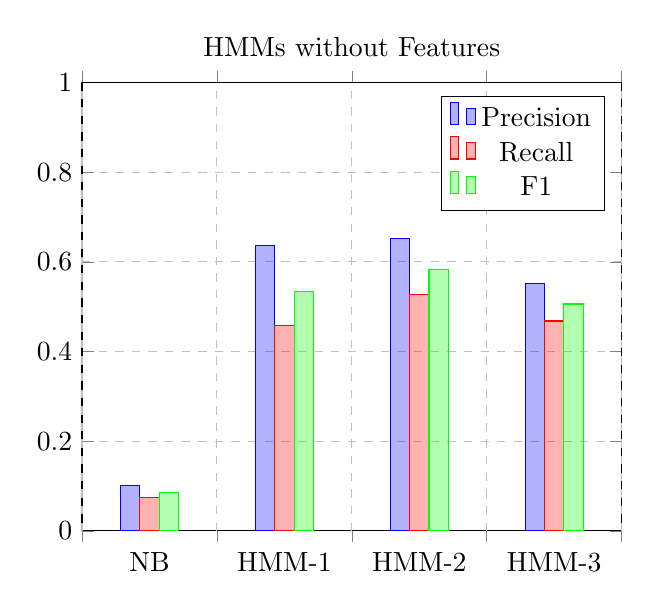
\begin{tikzpicture}
      \begin{axis}[
        title={HMMs without Features},
        xmin=0.5, xmax=4.5,
        ymin=0, ymax=1,
        xticklabels={NB,HMM-1,HMM-2,HMM-3},
        xtick={1,...,4},
        ytick={0,0.2,...,1},
        ybar=0pt,
        bar width=7pt,
        xtick distance=1,
        xtick style={
            /pgfplots/major tick length=0pt,
        },
        extra x ticks={-0.5,0.5,...,5.5},
        extra x tick labels=\empty,
        extra x tick style={
            grid=major,
            xtick style={
                /pgfplots/major tick length=4pt,
            },
        },
        ymajorgrids=true,
        grid style=dashed,
        legend pos=north east,
      ]

      \addplot[ybar, color=blue, fill=blue, fill opacity=0.3,] coordinates {
        (1,0.101)(2,0.637)(3,0.653)(4,0.551)
      };
      \addplot[ybar, color=red, fill=red, fill opacity=0.3,] coordinates {
        (1,0.075)(2,0.458)(3,0.527)(4,0.468)
      };
      \addplot[ybar, color=green, fill=green, fill opacity=0.3,] coordinates {
        (1,0.086)(2,0.533)(3,0.583)(4,0.506)
      };
      \legend{Precision, Recall, F1};
       
      \end{axis}
    \end{tikzpicture}
    \caption{
      Performance of the Naive Bayes classifier and Hidden Markov Models with no
      features besides the current word on the test set of the RNE dataset.
    }
    \label{fig:hmm_no_features}
  \end{center}
\end{figure}

\begin{table}[h]
  \small
  \begin{center}
    \begin{tabular}{ lllllll }
      \toprule
      \multirow{2}{*}{Model} & \multicolumn{3}{c}{Validation} & \multicolumn{3}{c}{Test} \\
                             & \multicolumn{1}{c}{P} & \multicolumn{1}{c}{R} & \multicolumn{1}{c}{F1}
                             & \multicolumn{1}{c}{P} & \multicolumn{1}{c}{R} & \multicolumn{1}{c}{F1} \\
      \midrule
      Naive Bayes    & 0.068 & 0.053 & 0.059 & 0.101 & 0.075 & 0.086   \\
      HMM-1          & 0.693 & 0.581 & 0.632 & 0.637 & 0.458 & 0.533 \\
      HMM-2          & 0.703 & 0.630 & 0.665 & \textbf{0.653} & \textbf{0.527} & \textbf{0.583} \\
      HMM-3          & 0.616 & 0.618 & 0.617 & 0.551 & 0.468 & 0.506 \\
      \bottomrule
    \end{tabular}
  \end{center}
  \caption{Performance of the Naive Bayes classifier and Hidden Markov Models with no
    features besides the current word on the validation and test sets of the RNE dataset.
  }
  \label{tab:hmm_no_features}
\end{table}

Considering label dependencies over multiple timesteps increases the classifier performance by a considerable margin 
relative to the Naive Bayes model even without any additional features. The 
second order HMM (HMM-2) achieved a $F_1$-score of 0.583 at the task, while
the Naive Bayes classifier achieved a $F_1$-score of only 0.086. All Hidden Markov Models are also 
better than the dictionary matching approach, which only achieved an $F_1$-score of 0.477. Nevertheless,
we already observe a relative decline in performance with the third order HMM (0.506 F1-score), 
suggesting that increasing the number of previous timesteps is not always advantageous. 
As we increase the window of previous labels at each timestep, the label combinations get less common
in the training set, and therefore, the probability estimates get less reliable.


\subsection{Feature selection}

Eleven discrete features were extracted from the dataset. 
These were selected from a larger pool of features, 
considering their aid to the performance of the extraction systems. Deep learning 
architectures can work incredibly well without any of these features, however they
are of critical importance to traditional approaches such as HMMs and CRFs. 
The selected features are presented in Table~\ref{tab:features}. 

\begin{table}[h]
  \small
  \begin{center}
    \begin{tabular}{ lll }
      \toprule
      Feature & Description & Type \\
      \midrule
      1  & Unaccented lowercase token & Categorical \\
      2  & Exact dictionary match & Binary \\
      3  & Partial dictionary match & Binary \\
      4  & Email & Binary \\
      5  & Number & Binary \\
      6  & Honorific (Mr., Mrs., Dr., etc.) & Binary \\
      7  & Matches a URL & Binary \\
      8  & Is capitalized & Binary \\
      9  & Is a punctuation sign & Binary \\
      10 & HTML tag + parent & Categorical \\
      11 & CSS class & Categorical \\
      \bottomrule
    \end{tabular}
  \end{center}
  \caption{
  Features used in the RNE dataset. Feature 10 is the token's enclosing HTML tag
  and its parent tag concatenated.
  }
  \label{tab:features}
\end{table}

The only features that demand further explanation are features 10 and 11.
Feature 10 is the token's enclosing HTML tag and its parent tag concatenated.
Feature 11 is the CSS class for the token's HTML tag.
Both of these features are only useful in the self-training strategy for HMMs and the
attention architectures for Bi-LSTM-CRFs. In other models, we use features 1 to 9.

%%% Review 3 
%%% Remove Partial Match from Group A

We know that correlated features may hurt the performance of \gls{hmm}s, because
we assumed feature independence to calculate the model parameters. So,
in Table~\ref{tab:feature_correlation} we present the feature correlation matrix based on 
the Cram�r's V measure, which is a correlation measure between two nominal variables. A value closer
to 0 means no correlation, a value close to 1 means complete correlation, and a value
close to -1 means inverse correlation, see~\cite{Cramer1946}. 
% The stronger correlations are shown in bold numbers.
% Dpython implementation
% https://en.wikipedia.org/wiki/Cram%C3%A9r%27s_V
% https://github.com/shakedzy/dython/blob/master/dython/nominal.py

\begin{table}[h]
  \tiny
  \begin{center}
    \begin{tabular}{ lccccccccccc }
      \toprule
           & \rot{Word} & \rot{Exact Match} & \rot{Partial Match} & \rot{Email} & \rot{Number} & \rot{Honorific} 
	   & \rot{URL} & \rot{Capitalized} & \rot{Punctuation} & \rot{HTML Tag} & \rot{CSS Class} \\
      \midrule
      Word          & 1.00 & \textbf{0.60} & \textbf{0.94} & \textbf{1.00} & \textbf{1.00}  & \textbf{1.00} & 0.00 & \textbf{0.84} & \textbf{1.00}  & 0.25 & 0.00 \\
      Exact Match   & -    & 1.00  & 0.19  & -0.02 & -0.07 & -0.04 & 0.00 & 0.15  & -0.05 & 0.07 & 0.22 \\
      Partial Match & -    & -     & 1.00  & -0.11 & -0.35 & -0.09 & 0.00 & -0.01 & 0.45  & 0.04 & 0.17 \\
      Email         & -    & -     & -     & 1.00  & -0.02 & -0.02 & 0.00 & -0.12 & -0.05 & 0.03 & 0.27 \\
      Number        & -    & -     & -     & -     & 1.00  & -0.07 & 0.00 & -0.36 & -0.16 & 0.09 & 0.34 \\
      Honorific     & -    & -     & -     & -     & -     & 1.00  & 0.00 & 0.15  & -0.08 & 0.02 & 0.11 \\
      URL           & -    & -     & -     & -     & -     & -     & 1.00 & 0.00  & 0.00  & 0.00 & 0.00 \\
      Capitalized   & -    & -     & -     & -     & -     & -     & -    & 1.00  & -0.48 & 0.07 & 0.28 \\
      Punctuation   & -    & -     & -     & -     & -     & -     & -    & -     & 1.00  & 0.04 & 0.11 \\
      HTML Tag      & -    & -     & -     & -     & -     & -     & -    & -     & -     & 1.00 & \textbf{0.64} \\
      CSS Class     & -    & -     & -     & -     & -     & -     & -    & -     & -     & -    & 1.00 \\
      \bottomrule
    \end{tabular}
  \end{center}
  \caption{Feature correlation matrix}
  \label{tab:feature_correlation}
\end{table}

The current word is strongly correlated with most features besides the URL feature and the ones related to 
the HTML structure. To understand how this can help or hurt the Hidden Markov Model performance we test the 
model using three groups of features:
%
\begin{itemize}
  \item Group A: Current word, Exact Match, Partial Match, URL, Capitalized
  \item Group B: All features except for the HTML Tag and the CSS Class
  \item Group C: The HTML Tag and the CSS Class
\end{itemize}
%
Group A is composed of features with a smaller correlation while Group B is composed of all the
textual features. Group C will only be used in the Self-Training strategy.

Figure~\ref{fig:hmm_features} compares the performance of HMMs using the 
features from Group A and Group B. Table~\ref{tab:hmm_features} presents the
numerical results for the same models.

\begin{figure}[h!]
  \begin{center}
    \tiny
    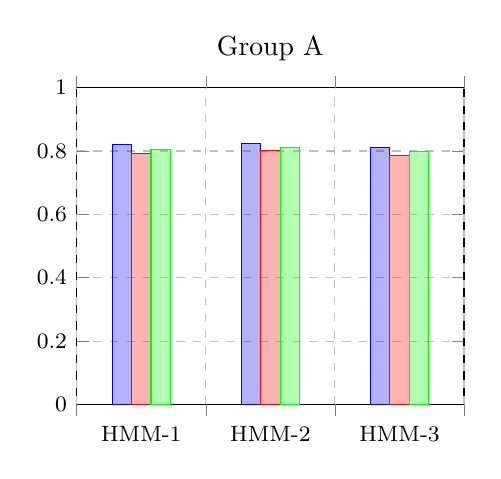
\begin{tikzpicture}
      \pgfplotsset{small}
      \begin{axis}[
        title={Group A},
        xmin=0.5, xmax=3.5,
        ymin=0, ymax=1,
        xticklabels={HMM-1,HMM-2,HMM-3},
        xtick={1,...,3},
        ytick={0,0.2,...,1},
        ybar=0pt,
        bar width=7pt,
        xtick distance=1,
        xtick style={
            /pgfplots/major tick length=0pt,
        },
        extra x ticks={-0.5,0.5,...,5.5},
        extra x tick labels=\empty,
        extra x tick style={
            grid=major,
            xtick style={
                /pgfplots/major tick length=4pt,
            },
        },
        ymajorgrids=true,
        grid style=dashed,
      ]

      \addplot[ybar, color=blue, fill=blue, fill opacity=0.3,] coordinates {
        (1,0.819)(2,0.823)(3,0.812)
      };
      \addplot[ybar, color=red, fill=red, fill opacity=0.3,] coordinates {
        (1,0.792)(2,0.802)(3,0.785)
      };
      \addplot[ybar, color=green, fill=green, fill opacity=0.3,] coordinates {
        (1,0.805)(2,0.812)(3,0.798)
      };
      \legend{};
       
      \end{axis}
    \end{tikzpicture}
    ~
    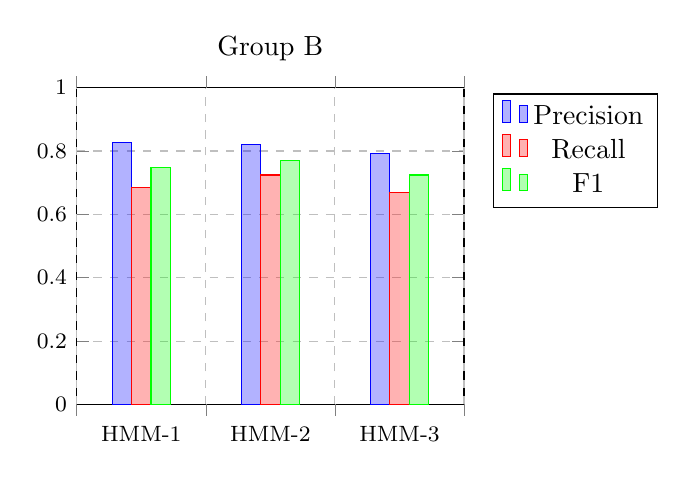
\begin{tikzpicture}
      \pgfplotsset{small}
      \begin{axis}[
        title={Group B},
        xmin=0.5, xmax=3.5,
        ymin=0, ymax=1,
        xticklabels={HMM-1,HMM-2,HMM-3},
        xtick={1,...,3},
        ytick={0,0.2,...,1},
        ybar=0pt,
        bar width=7pt,
        xtick distance=1,
        xtick style={
            /pgfplots/major tick length=0pt,
        },
        extra x ticks={-0.5,0.5,...,5.5},
        extra x tick labels=\empty,
        extra x tick style={
            grid=major,
            xtick style={
                /pgfplots/major tick length=4pt,
            },
        },
        ymajorgrids=true,
        grid style=dashed,
        % legend pos=north east,
	legend style={at={(1.5,0.8)},anchor=east},
      ]

      \addplot[ybar, color=blue, fill=blue, fill opacity=0.3,] coordinates {
        (1,0.826)(2,0.820)(3,0.791)
      };
      \addplot[ybar, color=red, fill=red, fill opacity=0.3,] coordinates {
        (1,0.684)(2,0.724)(3,0.668)
      };
      \addplot[ybar, color=green, fill=green, fill opacity=0.3,] coordinates {
        (1,0.748)(2,0.769)(3,0.724)
      };
      \legend{Precision, Recall, F1};
       
      \end{axis}
    \end{tikzpicture}

    \caption{Hidden Markov Models trained with the features in Group A and Group B.}
    \label{fig:hmm_features}
  \end{center}
\end{figure}

\begin{table}[h]
  \small
  \begin{center}
    \begin{tabular}{ lllllll }
      \toprule
      \multirow{2}{*}{Model} & \multicolumn{3}{c}{Validation} & \multicolumn{3}{c}{Test} \\
                             & \multicolumn{1}{c}{P} & \multicolumn{1}{c}{R} & \multicolumn{1}{c}{F1}
                             & \multicolumn{1}{c}{P} & \multicolumn{1}{c}{R} & \multicolumn{1}{c}{F1} \\
      \midrule
      HMM-1 (Group A)                 & 0.813 & 0.816 & 0.814 & 0.819 & 0.792 & 0.805 \\
      HMM-2 (Group A)                 & 0.787 & 0.820 & 0.803 & 0.823 & \textbf{0.802} & \textbf{0.812} \\
      HMM-3 (Group A)                 & 0.774 & 0.816 & 0.795 & 0.812 & 0.785 & 0.798 \\
      HMM-1 (Group B)                 & 0.730 & 0.714 & 0.722 & \textbf{0.826} & 0.684 & 0.748 \\
      HMM-2 (Group B)                 & 0.720 & 0.710 & 0.715 & 0.820 & 0.724 & 0.769 \\
      HMM-3 (Group B)                 & 0.721 & 0.702 & 0.711 & 0.791 & 0.667 & 0.724 \\
      \bottomrule
    \end{tabular}
  \end{center}
  \caption{
    Performance on the validation and test sets for Hidden Markov Models 
    trained with the features in Group A and Group B.
  }
  \label{tab:hmm_features}
\end{table}

The Group A models were better overall showing that too many correlated 
features can hurt the performance of \gls{hmm}s.
However, when these features are carefully selected, they can improve the 
performance of the \gls{hmm} significantly (0.812 F1 for the HMM-2)
relative to the performance of the featureless \gls{hmm} (0.583 F1 for the HMM-2).


\subsection{Self-training strategy}

In the next experiment, we wanted to understand if the self-training strategy described in
Section~\ref{sec:self_training} is effective for improving the performance of 
HMMs. Figure~\ref{fig:hmm_self_training} compares the performance of HMMs
up to third order with features from Group A and HMMs that 
were trained with Group A features and Self-Trained with Group C features. The numerical
results for the same models are presents in Table~\ref{tab:hmm_self_training}.

\begin{figure}[h!]
  \begin{center}
    \tiny
    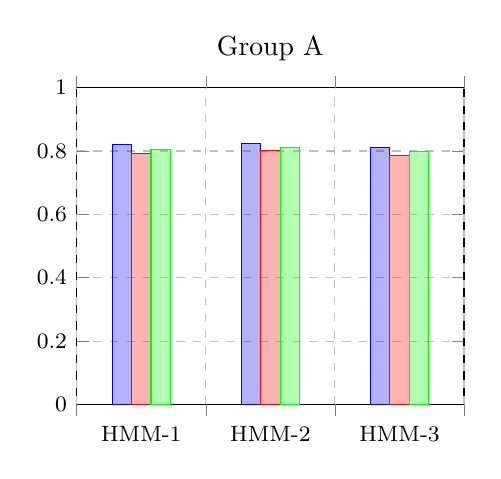
\begin{tikzpicture}
      \pgfplotsset{small}
      \begin{axis}[
        title={Group A},
        xmin=0.5, xmax=3.5,
        ymin=0, ymax=1,
        xticklabels={HMM-1,HMM-2,HMM-3},
        xtick={1,...,3},
        ytick={0,0.2,...,1},
        ybar=0pt,
        bar width=7pt,
        xtick distance=1,
        xtick style={
            /pgfplots/major tick length=0pt,
        },
        extra x ticks={-0.5,0.5,...,5.5},
        extra x tick labels=\empty,
        extra x tick style={
            grid=major,
            xtick style={
                /pgfplots/major tick length=4pt,
            },
        },
        ymajorgrids=true,
        grid style=dashed,
      ]

      \addplot[ybar, color=blue, fill=blue, fill opacity=0.3,] coordinates {
        (1,0.819)(2,0.823)(3,0.812)
      };
      \addplot[ybar, color=red, fill=red, fill opacity=0.3,] coordinates {
        (1,0.792)(2,0.802)(3,0.785)
      };
      \addplot[ybar, color=green, fill=green, fill opacity=0.3,] coordinates {
        (1,0.805)(2,0.812)(3,0.798)
      };
      \legend{};
       
      \end{axis}
    \end{tikzpicture}
    ~
    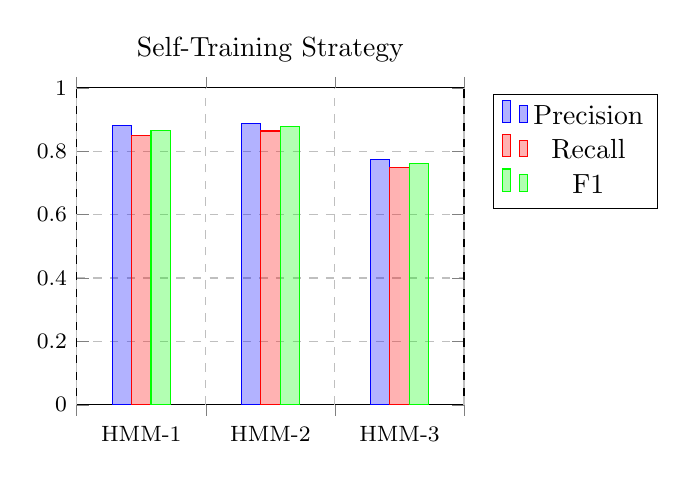
\begin{tikzpicture}
      \pgfplotsset{small}
      \begin{axis}[
        title={Self-Training Strategy},
        xmin=0.5, xmax=3.5,
        ymin=0, ymax=1,
        xticklabels={HMM-1,HMM-2,HMM-3},
        xtick={1,...,3},
        ytick={0,0.2,...,1},
        ybar=0pt,
        bar width=7pt,
        xtick distance=1,
        xtick style={
            /pgfplots/major tick length=0pt,
        },
        extra x ticks={-0.5,0.5,...,5.5},
        extra x tick labels=\empty,
        extra x tick style={
            grid=major,
            xtick style={
                /pgfplots/major tick length=4pt,
            },
        },
        ymajorgrids=true,
        grid style=dashed,
        % legend pos=north east,
	legend style={at={(1.5,0.8)},anchor=east},
      ]

      \addplot[ybar, color=blue, fill=blue, fill opacity=0.3,] coordinates {
        (1,0.880)(2,0.888)(3,0.774)
      };
      \addplot[ybar, color=red, fill=red, fill opacity=0.3,] coordinates {
        (1,0.850)(2,0.864)(3,0.750)
      };
      \addplot[ybar, color=green, fill=green, fill opacity=0.3,] coordinates {
        (1,0.865)(2,0.879)(3,0.762)
      };
      \legend{Precision, Recall, F1};
       
      \end{axis}
    \end{tikzpicture}

    \caption{
      HMMs trained with the features in Group A and HMMs trained with features 
      from Group A and self-trained with features from Group C.
    }
    \label{fig:hmm_self_training}
  \end{center}
\end{figure}

\begin{table}[h]
  \small
  \begin{center}
    \begin{tabular}{ lllllll }
      \toprule
      \multirow{2}{*}{Model} & \multicolumn{3}{c}{Validation} & \multicolumn{3}{c}{Test} \\
                             & \multicolumn{1}{c}{P} & \multicolumn{1}{c}{R} & \multicolumn{1}{c}{F1}
                             & \multicolumn{1}{c}{P} & \multicolumn{1}{c}{R} & \multicolumn{1}{c}{F1} \\
      \midrule
      HMM-1 (Group A) + Self-Training & 0.752 & 0.876 & 0.810 & 0.880 & 0.851 & 0.865 \\
      HMM-2 (Group A) + Self-Training & 0.784 & 0.892 & 0.835 & \textbf{0.888} & 0.864 & \textbf{0.879} \\
      HMM-3 (Group A) + Self-Training & 0.789 & 0.891 & 0.837 & 0.774 & 0.750 & 0.762 \\
      HMM-1 (Group B) + Self-Training & 0.747 & 0.906 & 0.819 & 0.866 & 0.867 & 0.866 \\
      HMM-2 (Group B) + Self-Training & 0.771 & 0.912 & 0.835 & 0.885 & \textbf{0.869} & 0.877 \\
      HMM-3 (Group B) + Self-Training & 0.788 & 0.917 & 0.847 & 0.826 & 0.803 & 0.814 \\
      \bottomrule
    \end{tabular}
  \end{center}
  \caption{
    HMMs trained with the features in Group A and HMMs trained with features 
    from Group A and self-trained with features from Group C. 
  }
  \label{tab:hmm_self_training}
\end{table}

The self-trained models show a marked improvement in comparison
to the models with no self-training at the test set except for the third order \textit{HMM}.
With this, we conclude that the best \textit{HMM} for the name extraction task is a 
second-order \textit{HMM} using \textit{Group A} features and the self-training strategy using
\textit{Group C} features. This model achieves a \textit{F1} of 0.879. 


\section{Conditional Random Fields}
\label{sec:experiments_crf}

%%% @ Review 9
%%% Retrain CRFs with cross validation.

When we compared a featureless Logistic Classifier with a featureless Naive Bayes model,
we found that the Logistic Classifier performed a little better. In this section we
want to check if featureless CRFs are also better than featuress HMMs. Also, CRFs provide a much more 
flexible way to incorporate 
features in comparison to HMMs. When considering the application
of this class of models to the Researcher Name Extraction task, we want to understand how the feature
selection impacts the performance of CRFs.

\subsection{No Features}

Figure~\ref{fig:crf_no_features} shows a comparison between the Logistic Classifier
(that assumes label independence), the best HMM without features (HMM-2)
and a CRF without features in the \gls{rne} task. Table~\ref{fig:crf_no_features} shows
the numerical results for the same models.

\begin{figure}[h!]
  \begin{center}
    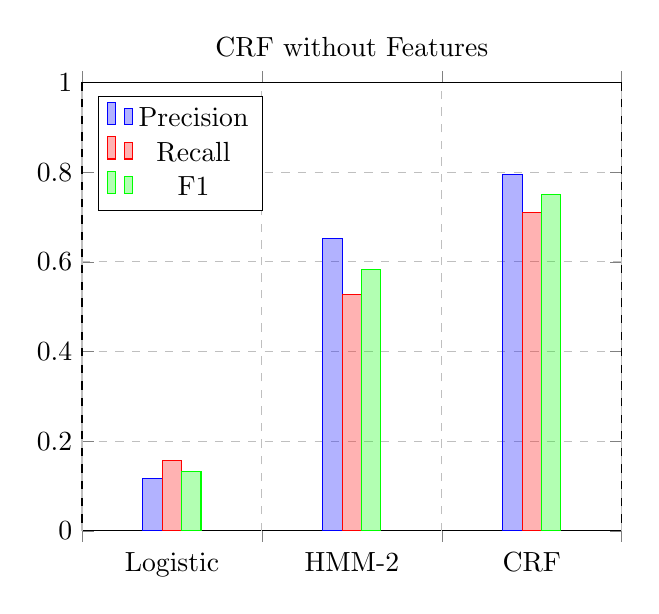
\begin{tikzpicture}
      \begin{axis}[
        title={CRF without Features},
        xmin=0.5, xmax=3.5,
        ymin=0, ymax=1,
        xticklabels={Logistic,HMM-2,CRF},
        xtick={1,...,3},
        ytick={0,0.2,...,1},
        ybar=0pt,
        bar width=7pt,
        xtick distance=1,
        xtick style={
            /pgfplots/major tick length=0pt,
        },
        extra x ticks={-0.5,0.5,...,5.5},
        extra x tick labels=\empty,
        extra x tick style={
            grid=major,
            xtick style={
                /pgfplots/major tick length=4pt,
            },
        },
        ymajorgrids=true,
        grid style=dashed,
        legend pos=north west,
      ]

      \addplot[ybar, color=blue, fill=blue, fill opacity=0.3,] coordinates {
        (1,0.116)(2,0.653)(3,0.795)
      };
      \addplot[ybar, color=red, fill=red, fill opacity=0.3,] coordinates {
        (1,0.156)(2,0.527)(3,0.710)
      };
      \addplot[ybar, color=green, fill=green, fill opacity=0.3,] coordinates {
        (1,0.133)(2,0.583)(3,0.750)
      };
      \legend{Precision, Recall, F1};
       
      \end{axis}
    \end{tikzpicture}
    \caption{
      Performance of the Logistic Classifier, second-order HMM and 
      CRF without features on the test set of the RNE dataset.
    }
    \label{fig:crf_no_features}
  \end{center}
\end{figure}

\begin{table}[h]
  \small
  \begin{center}
    \begin{tabular}{ lllllll }
      \toprule
      \multirow{2}{*}{Model} & \multicolumn{3}{c}{Validation} & \multicolumn{3}{c}{Test} \\
                             & \multicolumn{1}{c}{P} & \multicolumn{1}{c}{R} & \multicolumn{1}{c}{F1}
                             & \multicolumn{1}{c}{P} & \multicolumn{1}{c}{R} & \multicolumn{1}{c}{F1} \\
      \midrule
      Logistic Classifier    & 0.952 & 0.171 & 0.122 & 0.116 & 0.156 & 0.133 \\
      HMM-2 (featureless)    & 0.703 & 0.630 & 0.665 & 0.653 & 0.527 & 0.583 \\
      CRF (featureless)      & 0.806 & 0.805 & 0.806 & \textbf{0.795} & \textbf{0.710} & \textbf{0.750} \\
      \bottomrule
    \end{tabular}
  \end{center}
  \caption{
      Performance of the Logistic Classifier, second-order HMM and 
      CRF without features on the validation and test sets of the RNE dataset.
  }
  \label{tab:crf_no_features}
\end{table}

The CRF shows a significant improvement in comparison to the other models that used only the 
current word as a feature, achieving a F1-score of 0.750. Next, we proceed to understand if the addition 
of textual features can improve this performance further.


\subsection{Feature Selection}

To allow comparison between the HMMs from the last section, we consider CRFs using features
from Group A and Group B. Figure~\ref{fig:crf_all_features} shows a comparison between 
the best HMM and the CRFs using the features from Group A and Group B.
Table~\ref{tab:crf_all_features} presents the numerical results.

\begin{figure}[h!]
  \begin{center}
    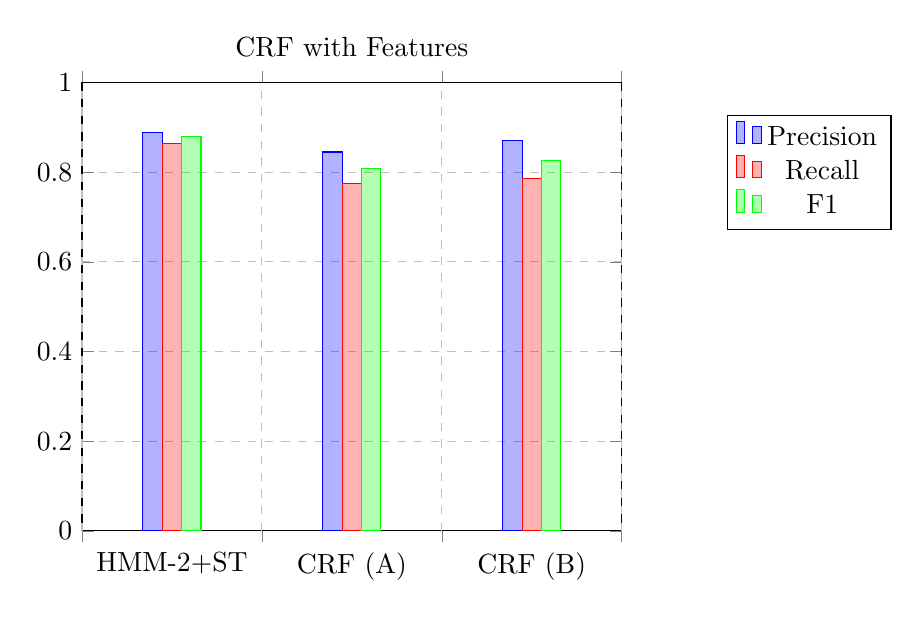
\begin{tikzpicture}
      % \pgfplotsset{small}
      \begin{axis}[
        title={CRF with Features},
        xmin=0.5, xmax=3.5,
        ymin=0, ymax=1,
        xticklabels={HMM-2+ST,CRF (A), CRF (B)},
        xtick={1,...,3},
        ytick={0,0.2,...,1},
        ybar=0pt,
        bar width=7pt,
        xtick distance=1,
        xtick style={
            /pgfplots/major tick length=0pt,
        },
        extra x ticks={-0.5,0.5,...,5.5},
        extra x tick labels=\empty,
        extra x tick style={
            grid=major,
            xtick style={
                /pgfplots/major tick length=4pt,
            },
        },
        ymajorgrids=true,
        grid style=dashed,
        % legend pos=north west,
	legend style={at={(1.5,0.8)},anchor=east},
      ]
      ]

      % HMM-2 (Group A) + Self-Training & 0.784 & 0.892 & 0.835 & \textbf{0.888} & 0.864 & \textbf{0.879} \\
      \addplot[ybar, color=blue, fill=blue, fill opacity=0.3,] coordinates {
        (1,0.888)(2,0.845)(3,0.870)
      };
      \addplot[ybar, color=red, fill=red, fill opacity=0.3,] coordinates {
        (1,0.864)(2,0.775)(3,0.786)
      };
      \addplot[ybar, color=green, fill=green, fill opacity=0.3,] coordinates {
        (1,0.879)(2,0.808)(3,0.826)
      };
      \legend{Precision, Recall, F1};
       
      \end{axis}
    \end{tikzpicture}

    \caption{
      CRFs trained with the features from Group A and Group B and the HMM-2 trained with features from Group A
      and self-trained with features from Group C. 
    }
    \label{fig:crf_all_features}
  \end{center}
\end{figure}


\begin{table}[h]
  \small
  \begin{center}
    \begin{tabular}{ lllllll }
      \toprule
      \multirow{2}{*}{Model} & \multicolumn{3}{c}{Validation} & \multicolumn{3}{c}{Test} \\
                             & \multicolumn{1}{c}{P} & \multicolumn{1}{c}{R} & \multicolumn{1}{c}{F1}
                             & \multicolumn{1}{c}{P} & \multicolumn{1}{c}{R} & \multicolumn{1}{c}{F1} \\
      \midrule
      HMM-2 (Group A) + Self-Training & 0.784 & 0.892 & 0.835 & \textbf{0.888} & \textbf{0.864} & \textbf{0.879} \\
      CRF (Group A)          & 0.857 & 0.875 & 0.866 & 0.845 & 0.775 & 0.808 \\
      CRF (Group B)          & 0.881 & 0.903 & 0.892 & 0.870 & 0.786 & 0.826 \\
      \bottomrule
    \end{tabular}
  \end{center}
  \caption{Conditional Random Fields using features from Group A and Group B.}
  \label{tab:crf_all_features}
\end{table}


The CRF is more robust to variations in the feature selection. It performs
similar to the second-order HMM in Group A and slightly better in Group B when we consider the HMMs
without the self-training strategy. However, when we consider the 
self-trained HMM-2, it still shows a better overall performance with an F1 score of 0.879.


\section{Neural Networks}
\label{sec:experiments_nn}

A neural network architecture that has had remarkable success at solving sequence labeling 
tasks is the Bi-LSTM-CRF described in Section~\ref{ssec:lstm_crf}. 
In Section~\ref{ssec:experiments_nn_1}, we investigate how featureless Bi-LSTM-CRFs compare to featureless HMMs and 
CRFs in the \gls{rne} task. In Section~\ref{ssec:experiments_nn_2}, we check if CNN-based or LSTM-based character 
representations can boost the performance of Bi-LSTM-CRFs in the same task. Lastly, in Section~\ref{ssec:experiments_nn_4}, we check if
the choice of pre-trained word embeddings alters the results significantly. 

Different from the previous models, that converged to an optimal set of parameters, the neural
networks must resort to numerical optimization methods over a rugged optimization function, therefore
they may get trapped in local minima and never find the best set of parameters. The results for the 
models may vary between different runs. Therefore we present the average results for each measure over
five runs of each model variation. 


\subsection{Bi-LSTM-CRF}
\label{ssec:experiments_nn_1}

%%% @ Review 10
%%% Retrain Bi-LSTM-CRFs with cross validation.

One of the advantages of deep neural networks relative to earlier sequence labeling methods is that they 
usually work without any feature engineering. 
Figure~\ref{fig:lstm_crf} compares the performance of a BI-LSTM-CRF on the test
set of the researcher name extraction task with the best HMMs and CRFs.
We only use GloVe-300 word embeddings as inputs to the Bi-LSTM-CRF model. Table~\ref{tab:lstm_crf_results}
presents the numerical results for the same models.

\begin{table}[h]
  \small
  \begin{center}
    \begin{tabular}{ lllllll }
      \toprule
      \multirow{2}{*}{Model} & \multicolumn{3}{c}{Validation} & \multicolumn{3}{c}{Test} \\
                             & \multicolumn{1}{c}{P} & \multicolumn{1}{c}{R} & \multicolumn{1}{c}{F1}
                             & \multicolumn{1}{c}{P} & \multicolumn{1}{c}{R} & \multicolumn{1}{c}{F1} \\
      \midrule
      HMM-2 (Group A) + Self-Training & 0.784 & 0.892 & 0.835 & 0.888 & 0.864 & 0.879 \\
      CRF (Group B)          & 0.881 & 0.903 & 0.892 & 0.870 & 0.786 & 0.826 \\
      Bi-LSTM-CRF           & 0.906 & 0.938 & 0.922 & \textbf{0.909} & \textbf{0.865} & \textbf{0.886} \\
      \bottomrule
    \end{tabular}
  \end{center}
  \caption{Results for the HMM using features from Group A and self-training, the CRF with features from Group B and the Plain Bi-LSTM-CRF.}
  \label{tab:lstm_crf_results}
\end{table}

\begin{figure}[h!]
  \begin{center}
    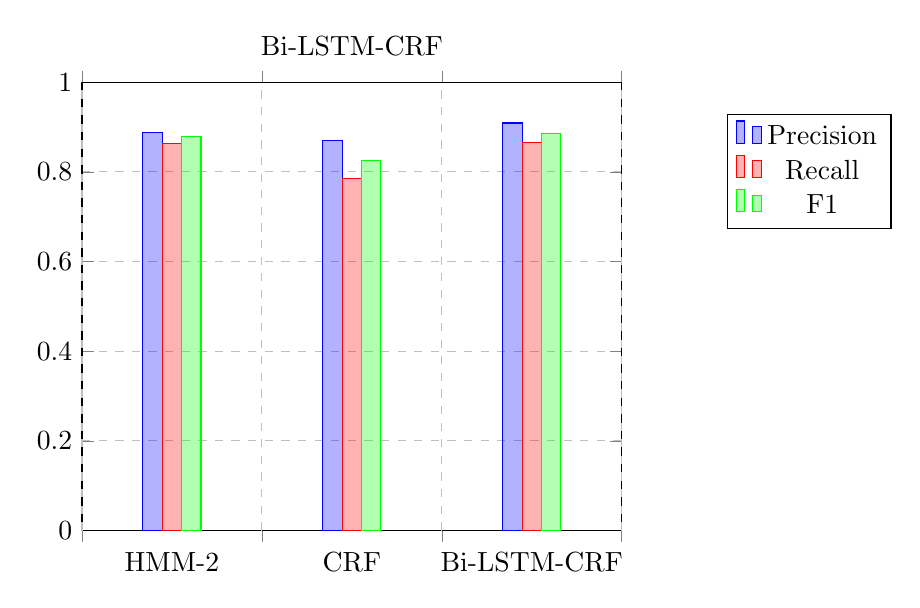
\begin{tikzpicture}
      \begin{axis}[
        title={Bi-LSTM-CRF},
        xmin=0.5, xmax=3.5,
        ymin=0, ymax=1,
        xticklabels={HMM-2,CRF,Bi-LSTM-CRF},
        xtick={1,...,3},
        ytick={0,0.2,...,1},
        ybar=0pt,
        bar width=7pt,
        xtick distance=1,
        xtick style={
            /pgfplots/major tick length=0pt,
        },
        extra x ticks={-0.5,0.5,...,5.5},
        extra x tick labels=\empty,
        extra x tick style={
            grid=major,
            xtick style={
                /pgfplots/major tick length=4pt,
            },
        },
        ymajorgrids=true,
        grid style=dashed,
        % legend pos=north west,
	legend style={at={(1.5,0.8)},anchor=east},
      ]
      ]

      \addplot[ybar, color=blue, fill=blue, fill opacity=0.3,] coordinates {
        (1,0.888)(2,0.870)(3,0.909)
      };
      \addplot[ybar, color=red, fill=red, fill opacity=0.3,] coordinates {
        (1,0.864)(2,0.786)(3,0.865)
      };
      \addplot[ybar, color=green, fill=green, fill opacity=0.3,] coordinates {
        (1,0.879)(2,0.826)(3,0.886)
      };
      \legend{Precision, Recall, F1};
       
      \end{axis}
    \end{tikzpicture}
    \caption{
      Performance of the Bi-LSTM-CRF with only GloVe embeddings in comparison to the HMM-2 (Group A) with
      self-training and the CRF (Group B).
    }
    \label{fig:lstm_crf}
  \end{center}
\end{figure}

The Bi-LSTM-CRF is better than the previous models, though the comparison is not 
completely fair, since we fed the model with word embeddings. However, these pre-trained embeddings 
are static and general to any language related task, so their incorporation in the model does not 
require any substantial effort. Without feature engineering, the Bi-LSTM-CRF model
already achieves an 0.886 F1-score, surpassing the best model discussed in the previous experiments (the HMM-2 with
self-training, which achieved 0.879 F1-score).


\subsection{Character Representations}
\label{ssec:experiments_nn_2}

Morphological features can help identifying named entities. We presented in Section~\ref{ssec:char_representations}
two methods for incorporating character representations in Recurrent Neural Networks, the CNN-based
method, and the LSTM-based method. In Table~\ref{tab:char_reps}, we compare the performance of
CNN character representations (CNNc) and LSTM character representations (LSTMc) with the plain Bi-LSTM-CRF. 
The character embeddings had 50 weights,
the CNN character representations used 50 filters with a window of size 3 and the LSTM-character 
representations used a bi-LSTM with 25 hidden states in each direction. Both techniques produced character
representations with 50 weights.

\begin{table}[h]
  \small
  \begin{center}
    \begin{tabular}{ lllllll }
      \toprule
      \multirow{2}{*}{Model} & \multicolumn{3}{c}{Validation} & \multicolumn{3}{c}{Test} \\
                             & \multicolumn{1}{c}{P} & \multicolumn{1}{c}{R} & \multicolumn{1}{c}{F1}
                             & \multicolumn{1}{c}{P} & \multicolumn{1}{c}{R} & \multicolumn{1}{c}{F1} \\
      \midrule
      Bi-LSTM-CRF           & 0.906 & 0.938 & 0.922 & 0.909 & 0.865 & 0.886 \\
      Bi-LSTM-CRF+CNNc      & 0.929 & 0.946 & 0.938 & \textbf{0.921} & 0.881 & 0.901 \\
      Bi-LSTM-CRF+LSTMc     & 0.928 & 0.950 & 0.939 & 0.920 & \textbf{0.886} & \textbf{0.902} \\
      \bottomrule
    \end{tabular}
  \end{center}
  \caption{Bi-LSTM-CRF with Character Representations.}
  \label{tab:char_reps}
\end{table}

The LSTM character representations improved the $F_1$-score by ~0.015 points relative to the plain
Bi-LSTM-CRF that only used GloVe-300 word embeddings. Also, both the 
CNN-based and the LSTM-based representations have a similar performance, yet 
the LSTM-based representations are slightly better, owing probably to the fact that they 
can represent prefixes and suffixes while the CNN-based filters are positional
invariant. 


\subsection{Word Embeddings}
\label{ssec:experiments_nn_4}

All neural architectures used in the experiments discussed in the previous Sections used GloVe-300 pre-trained word embeddings. However, the
choice of embeddings is of great importance to the success of neural sequence models. In fact, most
recent developments in NER models come from the incorporation of better pre-trained word embeddings 
to state-of-the-art models in many NLP tasks~\citep{Peters2018,Devlin2018}. We considered three sets of pre-trained word embeddings 
in our experiments: GloVe-300, Word2Vec-300 and ELMo. The characteristics of these
word embeddings is described in Table~\ref{tab:word_embeddings}. Different from GloVe-300 and Word2Vec-300, 
which are static, ELMo embeddings are context dependent and need to be recalculated for the specific dataset.
This adds significant overhead to the model training. While the Bi-LSTM-CRF with LSTM character embeddings and GloVe-300
embeddings took approximately 4,412 seconds to train and run predictions, the same model with ELMo embeddings took
approximately 9,437 seconds.
Table~\ref{tab:experiments_word_embeddings} compares the 
performance of Bi-LSTM-CRF models with LSTM-based character representations using different sets of pre-trained word embeddings.

\begin{table}[h]
  \small
  \begin{center}
    \begin{tabular}{ lllllll }
      \toprule
      \multirow{2}{*}{Model} & \multicolumn{3}{c}{Validation} & \multicolumn{3}{c}{Test} \\
                             & \multicolumn{1}{c}{P} & \multicolumn{1}{c}{R} & \multicolumn{1}{c}{F1}
                             & \multicolumn{1}{c}{P} & \multicolumn{1}{c}{R} & \multicolumn{1}{c}{F1} \\
      \midrule
      GloVe    & 0.928 & 0.950 & 0.939 & \textbf{0.920} & \textbf{0.886} & \textbf{0.902} \\
      Word2Vec & 0.925 & 0.926 & 0.926 & 0.899 & 0.831 & 0.864 \\
      ELMo     & 0.783 & 0.844 & 0.812 & 0.720 & 0.885 & 0.794 \\
      \bottomrule
    \end{tabular}
  \end{center}
  \caption{Bi-LSTM-CRF with LSTM characters and different sets of word embeddings.}
  \label{tab:experiments_word_embeddings}
\end{table}

GloVe embeddings are superior to Word2Vec in our NER setting, agreeing with the reported results for neural 
models in the {CoNLL-2003} English dataset for NER~\citep{Huang2015,Lample2016,Ma2016}. But, ELMo embeddings showed a very poor performance, 
contrasting with the results reported in the {CoNLL-2003} English dataset~\citep{Peters2018}. This is probably due to the fact that,
different from static embeddings, ELMo considers the context when generating word representations. The neural language
model that originates the embeddings was trained by~\cite{Peters2018} in text extracted from Wikipedia, so the contextual
representations generated by this language model are specifically tuned for plain text. ELMo seems to be highly reliant 
on this contextual information, but the HTML sentences in the \gls{rne} dataset provide very little context. Apparently, 
this specificity of the \gls{rne} dataset contributes negatively to the quality of the word embeddings.

The results obtained with different sets of embeddings are important because they show how the choice of 
word embeddings may influence the performance of a sequence model considerably. In fact, if we used Word2Vec embeddings
instead of GloVe embeddings, the Bi-LSTM-CRF would actually lose to the self-trained HMM-2, which reached a 0.879
$F_1$-score. Also, we cannot trust that only because an embedding shows superior performance in related tasks
that it will also be effective in the present task.


\subsection{Technical Details for Neural Networks}

All neural models were trained with the Adam Optimizer using a learning rate of 0.001 over 20 epochs on 
mini batches of size 10. We used early stopping~\citep{Caruana2000} to select the best parameters, considering 
the F1 measure in the validation set. All Bi-LSTM-CRF models contained a 
single LSTM layer with 100 weights. Dropout layers with 0.5 dropout rates were added after the LSTM, 
the character representations, and the attention matrix when applicable. The neural models were trained on 
Amazon G3.4xlarge instances, which have NVIDIA Tesla M60 GPUs with 8GB internal memory. The implementations
were made entirely in Python using Google's Tensorflow deep learning library~\footnote{https://www.tensorflow.org/.}. 


\section{What is the best model?}
\label{sec:experiments_best}

We reach the point where we try to answer the main question of this dissertation. 
We have experimented with multiple sequence labeling methods in the previous Sections and now we provide
an overview of the best variants of each category.
In Table~\ref{tab:best_models}, we compare the performance of the best HMMs, 
CRFs and Neural Networks for the \gls{rne} dataset.

\begin{table}[h]
  \small
  \begin{center}
    \begin{tabular}{ lllllll }
      \toprule
      \multirow{2}{*}{Model} & \multicolumn{3}{c}{Validation} & \multicolumn{3}{c}{Test} \\
                             & \multicolumn{1}{c}{P} & \multicolumn{1}{c}{R} & \multicolumn{1}{c}{F1}
                             & \multicolumn{1}{c}{P} & \multicolumn{1}{c}{R} & \multicolumn{1}{c}{F1} \\
      \midrule
       HMM-2 (Group A) + Self-Training    & 0.784 & 0.892 & 0.835 & 0.888          & 0.864          & 0.879 \\
       CRF (Group B)                      & 0.881 & 0.903 & 0.892 & 0.870          & 0.786          & 0.826 \\
       Bi-LSTM-CRF + LSTMc                   & 0.928 & 0.950 & 0.939 & \textbf{0.920} & \textbf{0.886} & \textbf{0.902}           \\
      \bottomrule
    \end{tabular}
  \end{center}
  \caption{Overview of the best models for the name extraction task in the RNE dataset.}
  \label{tab:best_models}
\end{table}

Taking the F1-score
as the comparison criterion, the Bi-LSTM-CRF model with LSTM 
character representations, and Glove-300 embeddings is the winning model with a
F1 of 0.902. 

Despite the superior performance of Neural Networks in this task, there remains an important 
consideration to be made. As we increase the complexity and training time required by our models, there 
is only a scant gain in terms of precision and recall. For example, the 
Bi-LSTM-CRF achieved an 0.902 F1-score, while 
the HMM-2 using a Self-Training strategy achieved a 0.879 
F1-score. This is a 0.023 increase, which is not insignificant, but it comes to mind if the additional
complexity is entirely justifiable. 

The Neural Network approach does not demand any feature engineering or self-training 
strategy, contrasting with the HMM approach, which is highly reliant on
the right selection of features and the self-training strategy. However, the absence of
human engineering in Neural Network training is questionable to some degree since we need to
define many hyper parameters and
many details about the neural architecture, such as the number of LSTM layers and
hidden weights, where to add dropout layers, which word embeddings to use, etc. In summary, 
there are many choices to be made, none of which have definitive theoretical justification, 
so the model variations need to be tested empirically. This means many iterations between setting
parameters, obtaining results, and tuning parameters once again. Considering that each of 
these iterations can take at least a couple of hours to finish, it is not clear if
selecting features is really a more arduous struggle.

To the best of our abilities, the Tensorflow implementation of the Bi-LSTM-CRF + LSTM chars
running on an AWS GPU instance took approximately 4,412 seconds to train 
and run predictions in the test set. While, the HMM-2 did the same in approximately
64 seconds, running in a conventional CPU with unoptimized code. That is roughly seventy times 
faster. Finally, if we consider the intellectual cost of understanding and implementing both 
models and the code maintainability of both implementations, the difference is even more profound.

Then, what is the best model? It depends on the end goal. If the goal is to achieve as much accuracy
as possible, then definitely go for Deep Neural Architectures. However, in most ordinary 
implementations, simpler models should probably be preferred. In both cases, models
trained on publicly available sequence tagging datasets will probably perform poorly,
so most of the effort would certainly be better spent on constructing task specific datasets
with a high quality. This points to the necessity of searching for good unsupervised approaches to 
sequence labeling. This way, we would have models with better flexibility and good accuracy in
many extraction tasks. Unfortunately, unsupervised and semi supervised approaches to this problem 
are still far from serviceable.


\chapter{Improvements to Neural Networks}

In the previous chapters, we discussed neural networks that can be generally employed in 
a diverse range of \gls{nlp} tasks. However, there are some specificities 
to the problem of sequence labeling on the Web that can be explored to allow further improvement 
of our models. Taking into consideration the success of the self-training strategy for
\gls{hmm}s, which is a form of incorporating knowledge about the HTML structure in the model,
we propose two experimental methods to boost the performance of neural networks when
sequence labeling Web documents.
In Section~\ref{sec:attention_models}, we propose two attention models
to incorporate HTML structural information in our neural sequence taggers.
In Section~\ref{sec:fscore_optimization}, we propose a new optimization objective for neural 
networks trained for sequence labeling tasks that can make them prioritize recall over precision,
what can be useful in a name extraction task on the Web.
Lastly, in Section~\ref{sec:new_experiments}, we discuss some experimental results for these 
strategies.


\section{Attentions Models} 
\label{sec:attention_models} 

The self-training strategy for HMMs demonstrates a way to incorporate HTML features in 
sequence models, however it is not clear how to apply the same intuition to Neural 
Networks. Ultimately, we want the model to consider the predictions that it made for 
words in similar HTML contexts when constructing the neural representation for the 
current word in a sequence. A natural way to incorporate this intuition into the neural 
architectures described in Section~\ref{sec:neural_networks} is with the use of 
attention mechanisms, similar to the one proposed by~\cite{Vaswani2017}.
An attention mechanism is a way to combine
inputs from multiple timesteps in a sequence to perform an operation at the current timestep.
Originally, attention mechanisms in \gls{nlp} were developed with the goal of solving 
sentence alignment for neural machine translation~\citep{Bahdanau2014}, but, since then, 
they found other uses.

In a Bi-LSTM-CRF model, the bidirectional \gls{lstm} layer produces output representations at each 
timestep, producing a $ T \times H $ matrix, where $ T $ is the number of timesteps in the
sequence and $ H $ is the \gls{lstm} hidden layer size, which is defined experimentally.
This matrix constitutes a neural representation for a sentence with vectors of size $ H $ representing
words at each timestep. Also, if the sequence length in the dataset varies, we can simply pad the short 
sentences with zero vectors. 

In the original Bi-LSTM-CRF model without an attention layer, the
neural representations would be passed directly to the \gls{crf} decoder, but in the Self-Attended 
Bi-LSTM-CRF, we add an attention mechanism between the \gls{lstm} output and the \gls{crf} input as described 
in Figure~\ref{fig:lstm_attention}.

\begin{figure}[h]
  \centering
  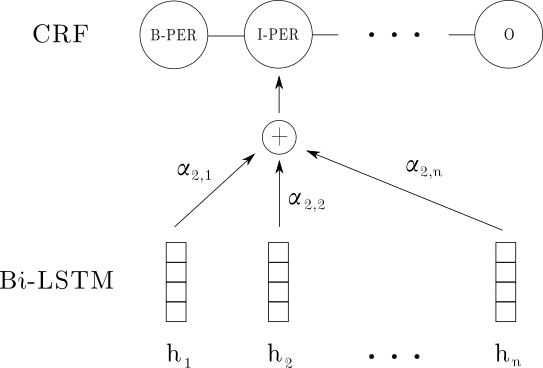
\includegraphics[width=0.5\textwidth]{pics/lstm_attention}
  \caption{Attention mechanism for the Bi-LSTM-CRF model.}
  \label{fig:lstm_attention}
\end{figure}

Now we need to find a way to combine the vectors at each timestep in a way that transforms 
the representations according to the similarity between HTML contexts. Essentially, we want to compute a $ T \times T $ 
attention matrix $ \alpha $ where $ \alpha_{i, j} $ is the weight attributed to the word representation $ h_j $ at timestep
$ i $. In other words, $ \alpha_{i, j} $ is measuring the amount of attention that we pay to each word $ j $ in
a sentence at timestep $ i $. With the $ \alpha $ matrix, we can calculate new representations $ h'_i $ 
for each timestep by performing a linear combination of the hidden states according to their 
attention values:

\begin{equation}
h'_i = \sum_{j} \alpha_{i, j} h_j
\end{equation}
Also, consider a set of $ n $ context vectors $ c_i $ that contain representations for the
HTML features at timestep $ i $. This representation can be a binary feature vector,
a dense vector or even the hidden states $ h_i $. The attention matrix is then calculated as:

\begin{equation}
\alpha_{i,j} = \frac{e^{A(c_i, c_j)}}{\sum_k e^{A(c_i, c_k)}}
\end{equation}
where $ A(c_i, c_j) $ is an attention function that computes the similarity between
HTML contexts at timesteps $ i $ and $ j $ and outputs a real number. The exponentials are
a Softmax normalization function to ensure that $ 1 \geq \alpha_{i,j} \geq 0 $ and 
$ \sum_{j} \alpha_{i, j} = 1 $. Next, we propose two ways for defining the attention function
$ A $. The Hard Attention Function and the Soft Attention Function. 

\subsection{Hard Attention Function}

The hard attention function is a binary similarity function that either outputs one when 
contexts are identical or zero when they are different. This definition only makes sense
when the contexts $ c_i $ at timestep $ i $ are discrete feature vectors, because otherwise 
we would need a softer comparability criterion. So, if $ c_i = \{ f_{i,1}, f_{i,2}, ..., f_{i,m} \} $
is a context vector where each feature $ f_{i,j} $ assumes a definite value from a discrete set
$ \gamma_j $, we can define the attention function:
%
\begin{equation}
  A(c_i, c_j) = \begin{cases} 
    1, \text{ if } f_{i,k} = f_{j,k} \;\;\; \forall \; k \in [1,m] \\ 
    0, \text{ otherwise}
  \end{cases}
\end{equation}
%
The combination of features must be sufficiently restrictive so that the mixture of hidden
states does not introduce too much noise. We have determined experimentally that considering
the enclosing HTML tag, its parent tag, and the CSS class as features is sufficient to 
allow a consistent comparison between similar HTML contexts. Ideally, the choice of features
could be performed automatically with the incorporation of a feed forward neural network in
the comparison function and a softer similarity criterion. A possibility for doing this is 
the Soft Attention Function.


\subsection{Soft Attention Function}

Different from the Hard Attention Function, the Soft Attention Function outputs a real number 
that represents the degree of similarity between HTML contexts. Now, instead of considering
discrete feature vectors we resort to dense vectorial representations for the HTML context.
We propose to extract HTML structural features with
DOM path representations. To do this, consider a DOM tree (which is an acyclic directed graph),
a word's HTML context can be represented by the path we take in this graph starting from the 
root element. If we consider the path for each word in our sequence, we can create HTML dense 
representations by training a matrix of fixed size embeddings for each HTML tag, then we construct 
HTML representations by averaging the embeddings in a final vector representation. The process
is described in Figure~\ref{fig:html_embeddings}. 

\begin{figure}[h]
  \centering
  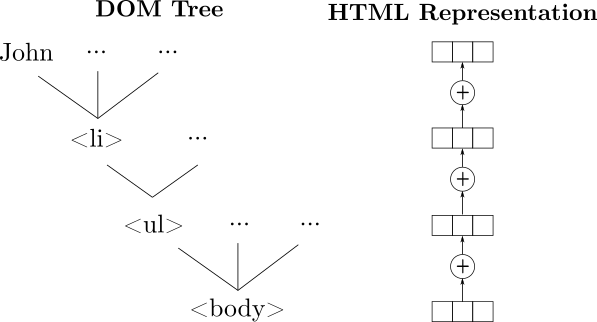
\includegraphics[width=0.5\textwidth]{pics/html_embeddings}
  \caption{Building HTML representations by climbing the DOM tree.}
  \label{fig:html_embeddings}
\end{figure}

Experimentally, we only considered the last two HTML embeddings, since the HTML tag 
information gets less relevant as we get farther from the leaves. The vocabulary of HTML 
tags is very small, so we can train HTML embeddings effectively in the target dataset. 
We could also learn HTML representations with CNNs or LSTMs as we did with character 
representations, instead of averaging the embeddings. 

Now to measure the similarity between different HTML contexts, we resort to an attention
function similar to the scaled dot product proposed by~\cite{Vaswani2017}. That is:

\begin{equation}
  A(c_i, c_j) = \frac{W c_i \cdot W c_j}{\sqrt{n}}
\end{equation}
where $ W $ is a weight matrix to be learned and $ \sqrt{n} $ is a normalization factor
with $ n $ being the size of the context vectors $ c $. This function assumes a larger
value when the contexts are similar and a smaller value when they are different. With the 
soft attention mechanism, our model can learn HTML context representations from the training 
data and produce generalization patterns such as "words happening together in a list probably 
belong to the same class".


\subsection{Dataset Split and Experimental Considerations}

In sequence labeling tasks, it is common to split the dataset in sentences and then train them
in independent steps. However, if we want to make use of attention mechanisms to 
perform the comparison of words in different HTML contexts, we want to compare labels attributed 
to words that share a similar context in different sentences. 
To allow the comparison of words in different sentences, instead of splitting the dataset into
independent shuffled sentences, we combine multiple sentences in a single training step and separate 
them with a segmentation token. Also, with the addition of many parameters to the model, the risk of 
overfitting increases. To prevent this problem from occurring, we added dropout layers with a 0.5 
dropout rate before and after the attention mechanism.


\section{F-score Optimization} 
\label{sec:fscore_optimization}

In the Bi-LSTM-CRF model, we estimate parameters by maximizing the log-likelihood. The likelihood is 
intimately associated with the accuracy in a classification task, but in NER tasks, models are 
usually evaluated according to their attained results in terms of precision, recall, or the F-score.
By maximizing the likelihood, we are essentially increasing accuracy with the expectation that this 
will lead to an improvement of the F-score, what is most often true. However, in extraction tasks 
there is usually a trade-off between precision and recall, meaning that we can trade a little less 
precision for an increase in recall and vice-versa. For example, if we want better
precision, it may be useful to throw away entities that were not classified with a high degree of 
confidence. Contrarily, if we want better recall, we can relax the classification criterium and 
extract entities that otherwise would be ignored. 

In NER on the Web, we could argue that recall is slightly more important than precision, because when 
parsing a huge amount of data, it is much easier to manually filter false positives than 
to manually find false negatives that were ignored by the classifier. This preference for recall
could be expressed in the evaluation by setting the F-score parameter $ \beta $ in a way that values recall twice 
as much as precision, for example. However, when maximizing the accuracy of a classifier
with the cross-entropy function, we have no way to tell the optimizer to choose parameters that maximize 
the F-score with a particular $ \beta $. We could try to maximize the F-score directly, but:

\begin{quote}
While the F-score of a classifier evaluated on a single supervised instance is well defined, the
overall F-score on a larger dataset is not a function of the F-score evaluated on each instance
in the dataset. This is in contrast to ordinary loss/utility, whose grand total (or average) on a dataset
can be computed by direct summation~\citep{Jansche2005}.
\end{quote}

This makes the usage of the F-score as an optimization objective impractical for large datasets trained in 
batches. However, with a few simplifications, we can replace our loss function and instead 
maximize the F-score in terms of a expected utility function. We take the method proposed by~\cite{Jansche2005}, that
approximately maximizes the F-score of a classifier based on a logistical regression model, and 
apply it to our neural architectures. The F-score function can then be calculated in terms of a triple (A,B,C), as follows:

\begin{equation}
F_\alpha(A, B, C) = \frac{A}{A + \alpha B + (1-\alpha) C}
\label{eq:falpha}
\end{equation}

This is equivalent to the $ \beta $-weighted harmonic mean defined in Equation~\ref{eq:fscore_formula}.
Variable $ A $ is the number of true positives, $ B $ is the number of false negatives, and $ C $ is the number 
of false positives. Table~\ref{tab:precision_recall} describes the relationship between the predictions and
the actual labels.

\begin{table}[h]
  \small
  \begin{center}
    \begin{tabular}{ cc|cc|c }
      \toprule
        & & \multicolumn{2}{c|}{Predicted}                               & \multirow{2}{*}{Total} \\
        & & \multicolumn{1}{c}{pos} & \multicolumn{1}{c|}{neg} & \\
      \midrule
      \multirow{2}{*}{Actual} & pos & A & B & $ n_{pos} $ \\  
                              & neg & C & D  & $ n_{neg} $ \\
      \midrule
        \multicolumn{2}{c|}{Total} & $ m_{pos} $   & $ m_{neg} $    & $ n $ \\
      \bottomrule
    \end{tabular}
  \end{center}
  \caption{Relationship between positive and negative matches.}
  \label{tab:precision_recall}
\end{table}

That is, $ n_{pos} $ is the number of positive examples in the dataset (true positives plus missed positives) 
and $ m_{pos} $ is the number of positive examples that were predicted (true positives plus false positives).
With this, we can rewrite $ F_\alpha(A, B, C) $ as:
%
\begin{equation}
F_\alpha(A, n_{pos}, m_{pos}) = \frac{A}{\alpha n_{pos} + (1-\alpha) m_{pos}}
\end{equation}
%
With this expression in mind, \cite{Jansche2005} proposes the following optimization objective
for the expected F-score:
%
\begin{equation}
\tilde{F}_\alpha(z, y) = 
  \frac{\tilde{A}(z, y)}
  {\alpha \tilde{n}_{pos} + (1-\alpha) \tilde{m}_{pos}(\theta)}
\end{equation}
%
where $ y = \{ y_1, y_2, \ldots, y_n \} $ is a vector of actual labels,
$ z = \{ z_{1}, z_{2}, \ldots, z_{n} \} $ is a vector of predictions,
and:
%
\begin{equation}
\theta_i \equiv \hat{P}(z_{i} = \textit{True}) \;\; \forall i \; \in \; [1, n]
\end{equation}
%
is the model probability that label $ z_i $ is a
\textit{True} label, assuming that we are dealing with a binary classification 
problem with only \textit{True} and \textit{False} labels. Finally,
%
\begin{align*}
\tilde{A}(y, z) & \equiv \sum_{i=1}^n I_{y_i = z_{i} = 1} \cdot \theta_i  \\
\tilde{m}_{pos}       & \equiv \sum_{i=1}^n \theta_i \\
\tilde{n}_{pos}       & \equiv \sum_{i=1}^n I_{y_i=1} - \tilde{A}(y, z)
\end{align*}
%
where $ I_{C} $ is an identity function that is equal to one when the clause $ C $ is true and zero otherwise.
With that, we have an optimization objective that can be optimized with standard numerical optimization methods.
As a simplification, we consider that each label is independent and belongs to a different entity. Further work 
is needed to resolve this simplification and to adapt this optimization function to multi-label classification 
tasks. But, as we will see in the experiments section,
this formulation is sufficient for the \gls{rne} task.


\section{Experiments} 
\label{sec:new_experiments} 

The techniques proposed in this chapter are still very experimental, but we will show 
some preliminary results by posing some additional research questions:
%
\begin{enumerate}
\item Can the hard-attention and soft-attention mechanisms boost the performance of the Bi-LSTM-CRF?
\item Can we control how much the Bi-LSTM-CRF values recall over precision?
\item Can we improve the results of the best models with a simple filtering strategy?
\end{enumerate}
%
In Section~\ref{ssec:experiments_nn_3}, we discuss the experiments concerning Research 
Question 1, in Section~\ref{ssec:experiments_nn_3}, we discuss the experiments concerning
Research Question 2, and lastly, in Section~\label{ssec:filter_false_positives}, we discuss
the experiments concerning Research Question 3.

\subsection{Attention Mechanisms}
\label{ssec:experiments_nn_3}

The Self-Training strategy for HMMs showed that there is a lot to gain
from incorporating features related to the HTML structure in our models. The HMM-2 
model improved from a 0.805 $F_1$-score to 0.879 $F_1$-score with the self-training strategy. 
The hard and soft attention mechanisms proposed in Section~\ref{sec:attention_models} are 
techniques for neural networks that attempt to bring improvements to the Bi-LSTM-CRF
in a manner similar to the self-training strategy for HMMs. 
In Table~\ref{tab:attention}, we compare the performance of 
the Bi-LSTM-CRF with LSTM-based character representations using a Hard Attention layer and 
a Soft Attention layer.

\begin{table}[h]
  \small
  \begin{center}
    \begin{tabular}{ lllllll }
      \toprule
      \multirow{2}{*}{Model} & \multicolumn{3}{c}{Validation} & \multicolumn{3}{c}{Test} \\
                             & \multicolumn{1}{c}{P} & \multicolumn{1}{c}{R} & \multicolumn{1}{c}{F1}
                             & \multicolumn{1}{c}{P} & \multicolumn{1}{c}{R} & \multicolumn{1}{c}{F1} \\
      \midrule
      
      Bi-LSTM-CRF + LSTMc       & 0.928 & 0.950 & 0.939 & 0.920 & 0.886 & 0.902 \\
      +Hard Attention           & 0.944 & 0.961 & 0.952 & \textbf{0.925} & \textbf{0.890} & \textbf{0.907} \\
      +Soft Attention           & 0.894 & 0.961 & 0.926 & 0.884 & 0.849 & 0.866 \\
      \bottomrule
    \end{tabular}
  \end{center}
  \caption{Hard and Soft Attention}
  \label{tab:attention}
\end{table}

The Hard Attention layer improved the original model by roughly 0.005 F1-score.
However, the Soft Attention layer actually decreased the performance, 
what demands further explanation. The Hard Attention layer captures if the HTML context 
between two tags is exactly the same, but it does not look at the context itself. 
What the Hard Attention layer learns is essentially how much it can trust 
predictions made for other words in the same HTML context, no matter what is the actual context. 
However, the Soft Attention layer, also learns features about the HTML context, because it 
transforms the contextual representations with a feed forward neural network and then
compares these neural representations. For example, the model could learn that tokens happening 
inside a list are more likely to be names, but since each document comes from a different
website, this reasoning is unlikely to be correct for most cases.
We cannot trust specific HTML configurations to be meaningful outside the document where they
happen. 
This does not mean that the Soft Attention layer is useless, but for it to grasp
abstract structural patterns that could be generally useful, we would need a much larger 
dataset. A possibility would be to pre-train unsupervised HTML contextual embeddings to detect
useful HTML patterns in a large collection and then use this knowledge in a specific sequence 
labeling setting.


\subsection{F-score Optimization}
\label{ssec:experiments_nn_5}

When training Deep Neural Networks for sequence labeling, we usually 
minimize the cross entropy. However, what we ultimately care about is the
F-score. In Section~\ref{sec:fscore_optimization}, we proposed to change the optimization objective
for Neural Networks and optimize the expected F-score function to control how much our model 
prioritizes recall over precision. 

The results presented in Chapter~\ref{cha:experiments} show that Neural Architectures tend 
to value precision over recall in the name extraction task, however it is arguably better to improve recall
and lose a little precision in this case, since it is easier to filter out false positives from the
results than to find the false negatives manually.

Figure~\ref{fig:fscore_optimization} presents the results on the test set 
for a Bi-LSTM-CRF model with LSTM character representations trained with the expected F-score 
optimization objective and varying the F-score $ \alpha $. For example, $ \alpha=0.5 $ means that we 
value recall as much as precision, $ \alpha=0.2 $ means that we value precision twice as much as recall, and 
$ \alpha=0.8 $ means that we value recall twice as much as precision. Take note that setting $ \alpha=0.5 $
does not mean that we are using the same model that minimizes the cross-entropy, because the optimization
objective is different.
The exact formula for the $F_\alpha$-score
was given in Equation~\ref{eq:falpha}. No attention layers were added to these models.

\begin{figure}[h!]
  \begin{center}
    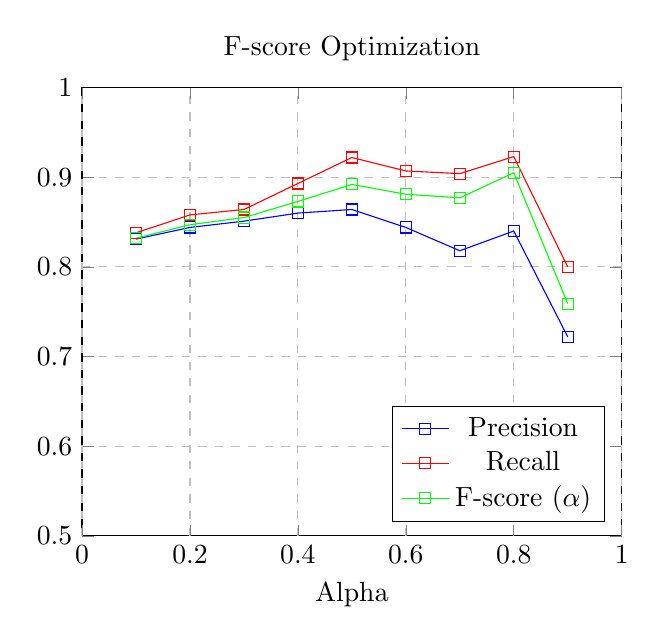
\begin{tikzpicture}
      \begin{axis}[
        title={F-score Optimization},
        xmin=0.0, xmax=1.0,
        ymin=0.5, ymax=1,
        xtick={0.0,0.2,...,1.0},
        ytick={0.5,0.6,...,1},
        xtick distance=1,
        xtick style={
            /pgfplots/major tick length=0pt,
        },
        xlabel={Alpha},
        extra x ticks={0.0,0.2,...,5.5},
        extra x tick labels=\empty,
        extra x tick style={
            grid=major,
            xtick style={
                /pgfplots/major tick length=4pt,
            },
        },
        ymajorgrids=true,
        grid style=dashed,
        legend pos=south east,
      ]


      \addplot[color=blue, color=blue,mark=square] coordinates {
        (0.1,0.831)(0.2,0.844)(0.3,0.851)(0.4,0.860)(0.5,0.864)(0.6,0.844)(0.7,0.818)(0.8,0.840)(0.9,0.722)
      };
      \addplot[color=red, color=red,mark=square] coordinates {
        (0.1,0.838)(0.2,0.858)(0.3,0.864)(0.4,0.893)(0.5,0.922)(0.6,0.907)(0.7,0.904)(0.8,0.923)(0.9,0.800)
      };
      \addplot[color=green, color=green,mark=square] coordinates {
	(0.1,0.832)(0.2,0.847)(0.3,0.855)(0.4,0.873)(0.5,0.892)(0.6,0.881)(0.7,0.877)(0.8,0.905)(0.9,0.759)
      };
      \legend{Precision, Recall, F-score ($ \alpha $)};
       
      \end{axis}
    \end{tikzpicture}
    \caption{
      Results for the Bi-LSTM-CRF + LSTMc that optimized the
      expected $F_{\alpha}$-score function. A larger $ \alpha $ means
      preference for recall rather than precision.
    }
    \label{fig:fscore_optimization}
  \end{center}
\end{figure}

This experiment shows that the capacity to control how much the model optimizes for one measure over the
other is limited. Even when giving a lot more priority to precision ($ \alpha=0.1 $), the model is still
less precise than the variant that optimizes for the $F_1$-score ($ \alpha=0.5 $). Actually, the model that achieves
top precision (0.864) and the second best recall (0.922) is the one with $ \alpha=0.5 $. The model with 
$ \alpha=0.8 $ achieves the best recall (0.923) and the best $ F_{\alpha} $ (0.905). However, 
in this case, there is a significant loss in precision while recall is not improved
substantially.

A useful result is that all of the models that optimized the expected F-score function 
valued recall over precision, contrasting with the Neural models that minimized the cross-entropy,
which prioritized precision over recall.
The Bi-LSTM-CRF that optimized the expected $F_1$-score obtained
a recall of 0.922 in the test set without losing a lot of precision (0.864), contrasting with the best model 
presented in the previous sections, the Hard-Attention Bi-LSTM-CRF, that achieved a 0.890 recall and 
0.925 precision. 
Table~\ref{tab:fscore_optimization} shows the detailed results for the models discussed in this Subsection.

\begin{table}[h]
  \small
  \begin{center}
    \begin{tabular}{ cllllll }
      \toprule
      \multirow{2}{*}{$\alpha$} & \multicolumn{3}{c}{Validation} & \multicolumn{3}{c}{Test} \\
                             & \multicolumn{1}{c}{P} & \multicolumn{1}{c}{R} & \multicolumn{1}{c}{$F_\alpha $}
                             & \multicolumn{1}{c}{P} & \multicolumn{1}{c}{R} & \multicolumn{1}{c}{$F_\alpha $} \\
      \midrule
       0.1 & 0.879 & 0.925 & 0.884 & 0.831 & 0.838 & 0.832 \\ 
       0.2 & 0.876 & 0.939 & 0.888 & 0.844 & 0.858 & 0.847 \\
       0.3 & 0.881 & 0.935 & 0.896 & 0.851 & 0.864 & 0.855 \\
       0.4 & 0.873 & 0.962 & 0.907 & 0.860 & 0.893 & 0.873 \\
       0.5 & 0.823 & 0.970 & 0.890 & \textbf{0.864} & 0.922 & 0.892 \\
       0.6 & 0.839 & 0.976 & 0.916 & 0.844 & 0.907 & 0.881 \\
       0.7 & 0.810 & 0.975 & 0.919 & 0.818 & 0.904 & 0.877 \\
       0.8 & 0.814 & 0.980 & 0.942 & 0.840 & \textbf{0.923} & \textbf{0.905} \\
       0.9 & 0.680 & 0.900 & 0.871 & 0.636 & 0.752 & 0.738 \\
      \bottomrule
    \end{tabular}
  \end{center}
  \caption{Bi-LSTM-CRF with LSTM character embeddings and F-score optimization objective.}
  \label{tab:fscore_optimization}
\end{table}


\subsection{Filtering False Positives}
\label{ssec:filter_false_positives}

In this dissertation, we argue that recall is more valuable than precision in NER
tasks on the Web. To verify this empirically, we consider the results of the best models
presented in Table~\ref{tab:best_models}, the Hard Attention Bi-LSTM-CRF and
the Bi-LSTM-CRF + LSTMc optimized for the F1-score, and apply a simple filter to the predicted
labels in the test set.
Despite their variations, all models tend to commit some
similar prediction mistakes. 

We tried a simple strategy to 
test how difficult it would be to filter out false positives from the results. The filtering strategy consists of automatically 
relabeling tokens that were labeled as a person ("B-PER" or "I-PER") to an outside ("O") label if:

\begin{enumerate}
\small
\item It was an honorific (Mr., Dr., P.hD., etc.).
\item It contained a number.
\item It was a punctuation sign just before or after a name (e.g. "- Mark" or "Emma ;").
\item It was an isolated name label.
\item It belonged to a name that was repeated at least three times.
\end{enumerate}

The results of this simple filtering strategy is presented in 
Table~\ref{tab:heuristic_filtering}. It improved the precision of all 
models considerably, showing that filtering out all false positives can probably be 
accomplished with only a small effort. 

\begin{table}[h]
  \small
  \begin{center}
    \begin{tabular}{ lllllll }
      \toprule
      Model + Filter (F) & Precision & Recall & F1 \\
      \midrule
       HMM-2 (Group A) + Self-Training       + F & 0.9240          & 0.8795          & 0.9012 \\
       CRF (Group B)                         + F & 0.9236          & 0.7951          & 0.8545 \\
       Bi-LSTM-CRF + LSTMc                   + F & \textbf{0.9387} & 0.8887          & 0.9130 \\
       Bi-LSTM-CRF + LSTMc + Hard Attention  + F & 0.9376          & 0.8997          & 0.9183 \\
       Bi-LSTM-CRF + LSTMc + F1 Optimization + F & 0.9239          & \textbf{0.9409} & \textbf{0.9323} \\
      \bottomrule
    \end{tabular}
  \end{center}
  \caption{Overview of the best models for the name extraction task in the RNE test set after the filtering strategy.}
  \label{tab:heuristic_filtering}
\end{table}

Lastly, in Table~\ref{tab:complexity} we present the training times and the subjective complexity 
for the best models in the RNE task. The subjective complexity tries to describe how much
effort a researcher has to put in order to implement and run tests with each model, considering our
particular experience in running the experiments for this dissertation.
As we increase the model complexity, we can raise the $ F_1 $ up to 0.9323 
with the F1 optimized Bi-LSTM-CRF + LSTMc after filtering false positives, what leaves small room 
for further improvement. 
However, with a much simpler model (the self-trained HMM-2) we can get a 0.9012 F1 after filtering false
positives, which is not significantly lower. These results are somewhat comparable to what has been 
happening with the reported results for the CoNLL-2003 English NER in the past few years 
(already discussed in Chapter~\ref{cha:related_work}). That is, as model complexity increases, the 
gains in terms of objective measures are not very substantial.


\begin{table}[h]
  \small
  \begin{center}
    \begin{tabular}{ lllllll }
      \toprule
      Model & F1 & F1 (after filter) & Time (seconds) & Complexity \\
      \midrule
       HMM-2 (Group A) + Self-Training & 0.879 & 0.9012 & 64   & Easy      \\
       CRF (Group B)                   & 0.826 & 0.8545 & 965  & Medium    \\
       Bi-LSTM-CRF + LSTMc             & 0.902 & 0.9130 & 4412 & Hard      \\
       +Hard Attention                 & 0.907 & 0.9183 & 6075 & Very Hard \\
       +F1 Optimization                & 0.892 & 0.9323 & 8065 & Very Hard \\
      \bottomrule
    \end{tabular}
  \end{center}
  \caption{Overview of the subjective complexity and training times of the best models for the RNE task.}
  \label{tab:complexity}
\end{table}


\chapter{Conclusions and Future Work}

Existing \gls{wde} methods are useful for extracting simple entities
from templated webpages, but they do not handle cross website extraction tasks
so well. Some techniques from machine learning such as \gls{ner} are 
much more flexible, but the existing models are usually concerned with 
extraction tasks in plain text, so there is an absence of datasets for Web named 
entity extraction tasks. In this dissertation, we introduced a novel dataset that 
handled the researcher name extraction task, the \gls{rne} dataset, and discussed 
the applicability of different machine learning approaches to this problem.

We assessed the performance of different types of \gls{hmm}s, \gls{crf}s
and Neural Networks in the \gls{rne} task, considering
their accuracy and complexity. We also proposed the self-training strategy for \gls{hmm}s
and the attentions models for Bi-LSTM-CRFs, inspired on \gls{wde} systems, to make use of 
HTML structural features and improve the model performances on the Web. Lastly,
we proposed to use a expected utility function based on the F-score as an optimization
objective for Neural Networks and prioritize recall over precision.

A natural extension of this work is to test the accuracy of the proposed models
on other Web extraction tasks. Naturally, this would require access to labeled 
datasets that concern these other tasks.


\section{Summary of Conclusions}

In this dissertation, we learned that machine learning methods for \gls{ner} are
useful for solving some cross-website data extraction tasks and, particularly, the
\gls{rne} task. We discussed the relative advantages and disadvantages of 
\gls{hmm}s, \gls{crf}s, and Neural Networks.
\gls{hmm}s and \gls{crf}s can solve the \gls{rne}
task with very good accuracy as long as we feed them with the correct features. Contrastingly,
Neural Networks demand no feature engineering and can obtain even better accuracy, however
their complexity and training time is not entirely justifiable since the gains are not very
substantial. In fact, Neural Networks cannot be considered entirely automatic, since we still 
have to tune hyper parameters and choose the right set of word embeddings. 

Additionally, both traditional methods and neural networks can profit from making use of
HTML structural features when used for sequence labeling in webpages. We proposed the self-training
strategy and the attention models to incorporate this knowledge in HMMs and Neural Networks, respectively.
And finally, we argued that we should value recall a little more that precision in Web extraction tasks, 
because filtering out false positives is easier than finding false negatives in the corpus. A way to
incorporate this intuition on Neural Network is through the optimization of the expected F-score utility
function. Also, we confirmed with the filtering strategy that filtering false negatives in the \gls{rne} task 
was indeed uncomplicated.


\section{Future Work}

This dissertation left many open ideas that could be explored in future research:

\begin{itemize}

\item \textbf{The self-training strategy} was very useful for improving the performance of HMMs,
but variations of this strategy could also be incorporated in neural architectures. The
hard-attention and soft-attention layers described in this dissertation were an early approach
for doing that, but they require further improvement. To make soft-attention layers more reliable,
we could pre-train HTML context embeddings in a large collection and derive structural
patterns that can be useful in many sequence labeling tasks in HTML.

\item \textbf{Good unsupervised methods} for \gls{wde} are necessary if we want
to solve this task definitively. NER methods trained in plain text become ineffective when 
they are applied to documents of a different type, so we end up having to construct new
datasets for each extraction task. This effort is very time-consuming, so we need more
flexible and accurate approaches. The Baum-Welch algorithm is an unsupervised method for
training HMMs, but it is not effective in NER. If we could devise an efficient way to
train semi supervised neural networks especially for Web extraction tasks, we could make 
an end-to-end system that solves NER, relationship extraction and named entity linking 
in a single step.

\end{itemize}

\section{Final Remarks}

The preliminary results of some of the Hidden Markov Models discussed in this dissertation 
were published in~\cite{deFreitasVeneroso2018}, though the results in this research article 
were not obtained with the exact same dataset. The other contributions in this dissertation
generated other two research articles that are still being reviewed. The first article makes a 
comparison of the P-score measure and the H-index, that was made possible by the collection of
affiliation information from university websites. The second article discusses the NER techniques 
proposed in this dissertation.

\ppgccbibliography{bibfile}

\end{document}
